\documentclass{FastFyp}
\usepackage{longtable}
\usepackage{booktabs}
\usepackage{array}
\usepackage{tabularx}
\usepackage{enumitem}
\usepackage{float}
\usepackage[table]{xcolor}
\usepackage{multirow}
\usepackage{microtype}
\usepackage{rotating}
\usepackage{xurl}
\usepackage{needspace}
\widowpenalty=10000 \clubpenalty=10000
\renewcommand{\floatpagefraction}{0.6}
\renewcommand{\textfraction}{0.1}
\setlist{nosep, leftmargin=*}
\newcolumntype{L}[1]{>{\raggedright\arraybackslash}p{#1}}
\newcolumntype{Y}{>{\raggedright\arraybackslash}X}

% ---------- Use-case table macro (template-compliant fields) ----------
\newenvironment{usecase}[2]{%
  \begin{table}[H]\centering\small
  \caption{#1}\label{#2}
  \begin{tabular}{|L{5.2cm}|L{\dimexpr\textwidth-5.2cm-4\tabcolsep-3\arrayrulewidth\relax}|}\hline}
  {\end{tabular}\end{table}}
\newcommand{\ucrow}[2]{\textbf{#1} & #2 \\ \hline}
\newcommand{\ucflow}[1]{\multicolumn{2}{|l|}{\textbf{#1}} \\ \hline \textit{Actor Action} & \textit{System Response} \\ \hline}
\newcommand{\ucstep}[2]{\textit{#1} & #2 \\ \hline}

% ---------- Metadata ----------
\newcommand{\supervisor}{Dr. Zareen Alamgir}
\newcommand{\university}{National University of Computer and Emerging Sciences, Lahore}
\newcommand{\fyptitle}{KhetLens: Offline, Context-Aware Crop Disease Diagnosis for Pakistani Farmers}
\newcommand{\degree}{BS}
\newcommand{\Studentone}{Ahsan Naeem \hspace{1.2em} 23L-0517 \hspace{1.2em} BS(CS)}
\newcommand{\Studenttwo}{Muhammad Taha Atif \hspace{1.2em} 23L-0657 \hspace{1.2em} BS(CS)}
\newcommand{\Studentthree}{Aaiza Iqbal \hspace{1.2em} 23L-0616 \hspace{1.2em} BS(CS)}
\date{October 2026}
\renewcommand{\contentsname}{Table of Contents}

\begin{document}

\makeatletter
    \begin{titlepage}
        
\includegraphics[width=0.2\linewidth]{Figures/nulogo.png}\hfill
        
\includegraphics[width=0.2\linewidth]{Figures/fast.png}\\
        \begin{center}
            {\large\bfseries \university}\\[5ex]
            
\includegraphics[width=0.36\linewidth]{Figures/fastlogo.png}\\[5ex]
            {\huge \bfseries KhetLens}\\[1.5ex]
            {\Large \bfseries Offline, Context-Aware Crop Disease Diagnosis\\ for Pakistani Farmers}\\[6ex]
            {\Studentone}\\[0.8ex]{\Studenttwo}\\[0.8ex]{\Studentthree}\\[3ex]
            {Supervisor: \supervisor} \\[1ex]
            {Industry Partner: Fatima Fertiliser Company Limited}\\[5ex]
            {Final Year Project -- I \quad (FYP ID: F26-141)}\\
            {Deliverable II: FYP Report}\\[1ex]
            {\large \@date}
        \end{center}
    \end{titlepage}
\makeatother
\frontmatter

\newpage \thispagestyle{empty} \mbox{} \newpage

\pagestyle{empty}
\section*{\begin{center}{Anti-Plagiarism Declaration} \end{center}}
This is to declare that the above publication was produced under the:
\begin{flushleft}
\bf Title: \fyptitle
\end{flushleft}
is the sole contribution of the author(s), and no part hereof has been reproduced as it is the basis (cut and paste) that can be considered Plagiarism. All referenced parts have been used to argue the idea and cited properly. I/We will be responsible and liable for any consequence if a violation of this declaration is determined.
\\[4ex]
Date: ..........................

\begin{flushright}
Name: Ahsan Naeem
\\[3ex]
Signature: ..........................
\\[6ex]
Name: Muhammad Taha Atif
\\[3ex]
Signature: ..........................
\\[6ex]
Name: Aaiza Iqbal
\\[3ex]
Signature: ..........................
\end{flushright}

\vspace{3 cm}
\hrule

\section*{Author's Declaration}
We, the authors of this report, declare that the work presented herein is our own and has not been submitted or presented previously to any other institution or organization for the award of any degree or qualification. Where the work of others has been used, it has been acknowledged and cited.
\pagebreak

\section*{Abstract}
KhetLens is a mobile application that helps farmers in Punjab identify common leaf diseases of wheat, maize and cotton from a photograph of the plant, taken close up or from a short distance, on an ordinary Android phone and without an internet connection. The diagnosis runs on the device using a compact deep learning model trained on field photographs from several regions and images collected locally with our industry partner. The image result is combined with recent local weather to separate diseases that look alike, and the app tells the farmer when it is not sure instead of guessing. Results, treatment guidance and a disease library are available in English, Urdu and Punjabi with audio. This report presents the project vision, literature review, requirements, methodology and design.
\pagebreak

\section*{Executive Summary}
Wheat, maize and cotton are the main field crops of Punjab, and leaf diseases are one of the most common reasons their yields fall short. Most farmers notice the symptoms themselves but have no quick way to confirm what they are seeing or what to do about it. Extension staff are few, and advice from input dealers is not always neutral. Many farming households, however, have access to an Android phone.

KhetLens puts a diagnosis tool on that phone. A farmer photographs the affected plant, close up or from a short distance; the app identifies the crop and the disease on the device, explains the result in the farmer's language with audio, and shows treatment and prevention guidance that has been reviewed with agronomists from our industry partner, Fatima Fertiliser Company Limited. A disease library and a short history of recent diagnoses are available without any network connection.

We have designed KhetLens around the conditions farmers actually face. It works fully offline, using the network only when available to refresh weather data, send feedback and download updates. It uses the recent weather of the farmer's district to help tell apart conditions that look similar in a photograph, such as rust and heat damage. It checks the photograph for blur and poor lighting, recognises when the photograph shows a crop or disease it does not know, and in those cases asks a few simple picture questions or says plainly that it is not sure. Where the app does give a confident answer, it explains why.

Technically, the app runs a compact MobileNetV3-based classifier compressed to 8-bit integers, with one shared backbone and separate output heads for the crop and for the diseases of each crop. The model is trained from public datasets of field photographs from several regions and from photographs collected locally with our partner. As part of the model-building work we will run a structured study to find how many local photographs are needed before further collection stops improving accuracy. The application is built natively for Android, stores its data locally, and talks to a small backend service for one-time verification, feedback collection and updates.

The report is organised as follows. Chapter 1 introduces the document. Chapter 2 presents the project vision: the problem, our goals, the scope and the stakeholders. Chapter 3 reviews the literature and related applications. Chapter 4 specifies the software requirements, interface and data design. Chapter 5 describes our proposed approach and methodology. Chapter 6 gives the high-level and low-level design.
\pagebreak


\pagestyle{fancy}
\tableofcontents
\pagebreak
\addcontentsline{toc}{chapter}{List of Figures}
\listoffigures
\pagebreak
\addcontentsline{toc}{chapter}{List of Tables}
{\setlength{\cftbeforetabskip}{3pt}\listoftables}

\mainmatter

\chapter{Introduction}
\label{ch:intro}

Crop disease is a routine part of farming in Punjab, and for wheat, maize and cotton it is also one of the main reasons a season's yield falls short. Wheat alone covers close to ten million hectares in Pakistan, and maize and cotton together add another four million~\cite{fao_pakistan}. Most leaf diseases of these crops are visible early and are treatable if they are recognised in time. The difficulty for a smallholder is recognising them: an agricultural officer may be far away, a neighbour's guess may be wrong, and a dealer has products to sell. The one tool many farming households now have is a smartphone.

Deep learning has made it possible to recognise plant diseases from photographs with high accuracy. Since the PlantVillage work of 2016 reported over 99\% accuracy on a large set of leaf images~\cite{mohanty2016}, many studies have reported similar results. The same body of work also showed something that matters more for a real product: models trained on clean, laboratory-style photographs do much worse on photographs taken in actual fields, with cluttered backgrounds, uneven light and mixed symptoms~\cite{xu2024datasets,singh2020plantdoc}. A useful farmer-facing application therefore has to be trained and tested on field conditions, has to run on the kind of phone farmers own, has to work without an internet connection, and has to speak the farmer's language.

KhetLens is our response to this. It is a mobile application that diagnoses leaf diseases of wheat, maize and cotton from a photograph of the plant, whether a close-up of a leaf or a wider shot showing several leaves, entirely on the phone, and presents the result with treatment guidance in English, Urdu and Punjabi. We have scoped it as a complete product rather than a model alone, and as a research and development project, because several of its parts address open questions: how much locally collected field data is needed, whether simple context such as recent weather can help separate diseases that look alike, and how a small on-device model can reliably recognise when it should not answer. We are carrying out the project with Fatima Fertiliser Company Limited, who are supporting us with field access and agronomic expertise.

\section{Purpose of this Document}
This document presents the vision, requirements, methodology and design of KhetLens as they stand at this deliverable. Its purpose is to describe clearly what we are building and why, to show that the design rests on the relevant literature, and to provide the specification against which the implementation will be developed and tested.

The project is guided by four research questions:
\needspace{6\baselineskip}
\begin{itemize}
  \item \textbf{RQ1.} How well does a compact, on-device model for wheat, maize and cotton leaf disease generalise from public datasets to field photographs, and what training choices improve that generalisation?
  \item \textbf{RQ2.} How many locally collected field photographs per class are needed, on top of public datasets, before additional collection gives little further improvement?
  \item \textbf{RQ3.} Does combining the image result with recent local weather improve the separation of visually similar conditions?
  \item \textbf{RQ4.} Can a lightweight uncertainty check running on the phone reliably recognise poor photographs, unsupported crops and unfamiliar diseases?
\end{itemize}

Our methods are empirical: we assemble image datasets, train and compress a classifier, measure it on field photographs and on the target class of phone, and run the controlled experiments described in Chapter~\ref{ch:method}. The report describes the design as planned; the implementation, test cases and results will follow in the subsequent deliverables.

\section{Intended Audience}
The report is written for three readers. The first is the FYP evaluation panel and our supervisor at the FAST School of Computing, who will assess whether the problem is well defined, the literature review is sound, the requirements are complete and the design is implementable; Chapters~\ref{ch:lit}, \ref{ch:method} and \ref{ch:design} are written mainly for them. The second is our industry partner, whose agronomists will review the disease list and the treatment content; Chapters~\ref{ch:vision} and \ref{ch:srs} describe the product in terms they can check without the technical detail. The third is ourselves, for whom Chapters~\ref{ch:srs} to \ref{ch:design} are the working specification.

\section{Definitions, Acronyms, and Abbreviations}
\label{sec:acronyms}
\begin{description}[style=nextline, leftmargin=0pt, itemsep=1pt]
  \item[Abiotic stress] Plant damage from non-living causes such as heat or nutrient shortage, which can resemble disease on a leaf.
  \item[API] Application Programming Interface.
  \item[CLCuV] Cotton Leaf Curl Virus.
  \item[CNN] Convolutional Neural Network.
  \item[Content pack] The bundle of disease, treatment and audio content shipped with the app and updated independently of the code.
  \item[FYP] Final Year Project.
  \item[GLS] Grey Leaf Spot (maize).
  \item[INT8] 8-bit integer representation used for compressed neural networks.
  \item[KD] Knowledge Distillation: training a small model to imitate a larger one.
  \item[NLB] Northern Leaf Blight (maize).
  \item[OOD] Out-of-Distribution: an input unlike the training data.
  \item[OTP] One-Time Password, used for sign-in.
  \item[SDG] Sustainable Development Goal.
  \item[Shahmukhi] The Perso-Arabic script used for Punjabi in Pakistan.
  \item[SRS] Software Requirement Specification.
  \item[TFLite / LiteRT] Google's runtime for running neural networks on mobile devices.
\end{description}

\section{Conclusion}
This chapter has introduced the problem KhetLens addresses, the purpose and readers of the report, and the terms used in it. The rest of the report is organised as follows. Chapter~\ref{ch:vision} presents the project vision: the problem domain, problem statement and elaboration, goals, scope, SDG, constraints, business opportunity and stakeholders. Chapter~\ref{ch:lit} reviews the literature and related applications and summarises them in a table. Chapter~\ref{ch:srs} gives the software requirements: features, functional and non-functional requirements, use cases, hardware and software, the user interface, the database design and the risk analysis. Chapter~\ref{ch:method} describes our proposed approach and methodology. Chapter~\ref{ch:design} presents the high-level and low-level design.

\chapter{Project Vision}
\label{ch:vision}

This chapter describes what KhetLens is for. We first give an overview of the problem domain and a description of the system, then state the problem and break it into its parts. We then list our goals and objectives, define the scope, identify the Sustainable Development Goals the project supports, and record the constraints, the business opportunity and the stakeholders.

\section{Problem Domain Overview}
\label{sec:domain}
KhetLens sits where three areas meet: smallholder farming in Punjab, image-based plant pathology, and machine learning on low-cost phones.

Wheat is Pakistan's largest crop by area, with maize and cotton following among the field crops~\cite{fao_pakistan}; maize is grown in two seasons and supplies the poultry and livestock sector, and cotton is the main fibre crop of southern Punjab and the base of the textile industry. All three are grown mostly on small holdings. When a disease appears, the farmer relies on experience, neighbours, the local dealer, and occasional visits from extension staff. Timely, reliable diagnosis is the exception rather than the rule.

Many of the most damaging diseases of these crops show clearly on a leaf: the yellow stripes of wheat stripe rust, the scattered brown pustules of leaf rust, the long grey-brown lesions of maize northern leaf blight, the upward curling and thickened veins of cotton leaf curl. These are the symptoms a farmer notices and a phone camera can capture, whether in a close-up of one leaf or in a photograph of the plant taken from a short distance. A few conditions look alike in a photograph, for instance early rust and heat scorch, or bacterial blight and fungal leaf spot in cotton. Agronomists tell them apart using context, and the recent weather is one of the most useful clues, because fungal and viral epidemics are closely tied to temperature and humidity~\cite{ali2023striperust,ahmad2018clcuv}.

The phones farmers carry are entry-level Android devices with a few gigabytes of memory and no reliable connectivity. Modern mobile network architectures and model compression techniques~\cite{howard2019mnv3,hinton2015kd} make it practical to run a disease classifier on such a phone, provided the model is small, quantised and bundled with everything it needs.

\textbf{What the system does.} A farmer opens KhetLens, which has already fetched and stored the recent weather of their district the last time the phone was online. They photograph the affected plant, close up or from a short distance so that several leaves are visible. On the phone, the photo is checked for blur and poor lighting, analysed as a whole and in regions by a compact neural network that identifies the crop and the disease, scored for how confident and how familiar the result is, and adjusted using the recent weather. If the result is confident, the farmer sees the disease name in their language with an audio explanation and the reasons for the decision, and can open treatment and prevention guidance. If two conditions are close, the app asks up to three simple picture questions. If the photo is poor or shows something the model does not know, the app says so and suggests taking more photos rather than guessing. Each diagnosis is kept in the history for six months, and the farmer can report whether the diagnosis and treatment worked; that feedback is sent when the phone next has a connection and then removed from the phone. A library of all supported diseases, with audio, is available offline.

\section{Problem Statement}
Smallholder farmers in Punjab do not have quick, trustworthy access to leaf disease diagnosis for wheat, maize and cotton. Existing tools generally need an internet connection, are built and tested on laboratory-style images rather than field photographs, always give an answer even when the input is unclear, and present advice in languages and from sources that do not fit the local farmer. An offline, Urdu- and Punjabi-speaking application that diagnoses these three crops on an ordinary phone, uses local context to resolve look-alike symptoms, admits uncertainty, and gives locally reviewed treatment guidance is what we set out to build; we have not found an existing application that does this.

\section{Problem Elaboration}
We see the problem as four connected sub-problems.

\subsection{Working on real field photographs}
Published classifiers reach very high accuracy on curated datasets but lose a large part of it on photographs taken in fields, where the background, lighting, distance and framing vary and symptoms appear at different stages~\cite{mohanty2016,singh2020plantdoc}. Part of the cause is that models learn from the background and the photographic style as much as from the leaf~\cite{noyan2022bias}. Our model therefore has to be trained on field photographs from several regions, taken at a range of distances, augmented to reduce background shortcuts, tested only on field photographs, and complemented by photographs we collect locally.

\subsection{Telling apart conditions that look alike}
\label{sec:pairs}
Some pairs of conditions cannot be reliably separated from a single leaf image. For evaluation we designate three such pairs: rust against abiotic heat stress in wheat and maize; bacterial blight against fungal leaf spot in cotton; and leaf reddening against leaf curl virus in cotton. The recent weather is a cheap and available signal: stripe rust in Punjab, for example, develops within a specific range of temperature and humidity~\cite{ali2023striperust}, while heat scorch follows hot, dry spells. We need a way to use this signal that does not require a large paired dataset of images and weather.

\subsection{Knowing when not to answer}
A diagnosis tool that always answers can send a farmer to buy the wrong spray. The app has to recognise three different situations: a photograph too blurred or dark to use; a crop or object it was not trained on; and a disease of a supported crop that it has not seen. Each needs a different check and a different response (retake, decline, or ask questions), and all of them have to run on the phone. Plain softmax confidence is known to be over-confident~\cite{guo2017calibration}, so better-founded measures are needed.

\subsection{Reaching the farmer}
The application must work with no connection, on an entry-level phone, for a user who may read little and prefers Punjabi or Urdu. This means on-device inference, an icon-first interface, audio on every screen, locally reviewed treatment content, and an interface that explains its answers so that farmers come to trust it. Studies of agricultural advisory apps find that trust and visible results are what drive farmers' intention to adopt a tool~\cite{soodan2024adoption}.

\section{Goals and Objectives}
\label{sec:goals}
Our goal is to give wheat, maize and cotton farmers in Punjab a trustworthy, offline disease diagnosis tool in their own language. The objectives are:
\begin{enumerate}[label=\textbf{O\arabic*},leftmargin=2.2em]
  \item Diagnose the common leaf diseases of wheat, maize and cotton from a photograph of the plant, close up or from a short distance, with the model running on the phone.
  \item Run on entry-level Android phones, with a diagnosis returned within a couple of seconds and all farmer-facing features working offline.
  \item Use recent local weather to improve the separation of visually similar conditions.
  \item Recognise unusable photographs, unsupported crops and unfamiliar diseases, and respond with a retake request, follow-up questions or an honest ``not sure'' rather than a guess.
  \item Determine, through a structured study, how many locally collected field photographs are needed on top of public datasets.
  \item Present diagnoses, questions and guidance in English, Urdu and Punjabi with audio.
  \item Provide an offline disease library and an automatic short-term history of diagnoses.
  \item Base treatment guidance on Pakistani advisories and agricultural research, reviewed with our partner's agronomists.
  \item Collect farmer feedback on diagnosis and treatment outcomes to improve the system over time.
\end{enumerate}
We will measure O1 to O5 on a held-out set of field photographs and on the target class of phone, using accuracy and macro-F1, inference time and model size, calibration error and the false-positive rate of the uncertainty check; O6 to O9 will be verified through content review, test cases and feedback from farmers and field staff.

\section{Project Scope}
\label{sec:scope}
KhetLens covers three crops, wheat, maize and cotton, chosen for their area in Punjab and their importance to farmers. Within them it covers the conditions in Table~\ref{tab:classes}, selected because they are common in the region, visible on a leaf, and covered by available training data. The list will be confirmed with our partner's agronomists; fall armyworm damage in maize is a possible addition.

\begin{table}[H]
\centering\small
\caption{Conditions covered by KhetLens (17 classes).}
\label{tab:classes}
\begin{tabularx}{\textwidth}{|L{1.8cm}|Y|}
\hline
\textbf{Crop} & \textbf{Conditions} \\ \hline
Wheat (6) & Yellow (stripe) rust; brown (leaf) rust; powdery mildew; leaf blight / spot blotch; abiotic stress (heat scorch, nutrient deficiency); healthy \\ \hline
Maize (5) & Northern leaf blight; common rust; grey leaf spot; abiotic stress; healthy \\ \hline
Cotton (6) & Cotton leaf curl virus; bacterial blight; fungal leaf spot (Alternaria, target spot); leaf reddening; sucking-pest damage (whitefly, jassid); healthy \\ \hline
\end{tabularx}
\end{table}

\subsection{In scope}
\begin{itemize}
  \item Core diagnosis: on-device identification of crop and condition from a photograph of the plant, close up or from a short distance, fully offline.
  \item Context-aware diagnosis: adjustment of the image result using the recent weather of the farmer's district.
  \item Uncertainty handling: blur and exposure check, detection of unsupported or unfamiliar inputs, up to three picture-based follow-up questions, and an explicit ``not sure'' outcome.
  \item A three-language interface (English, Urdu, Punjabi) with recorded audio for all content.
  \item An offline disease library covering every supported condition.
  \item An automatic diagnosis history, kept for six months and then cleared.
  \item Treatment and prevention guidance drawn from Pakistani advisories and research, reviewed with agronomists, with the source shown.
  \item A farmer feedback mechanism that works offline and syncs when connected.
  \item Phone-number sign-in with a one-time code sent over WhatsApp, and a guest mode so that diagnosis never requires an account.
  \item Model and content updates downloaded when connected, without reinstalling the app.
  \item A small backend for verification, feedback collection and distribution of updates.
  \item A field-data efficiency study, carried out as part of model building rather than as a farmer-facing feature.
\end{itemize}

\subsection{Out of scope}
\begin{itemize}
  \item Crops other than wheat, maize and cotton, and diseases that show on stems, spikes, bolls or roots rather than leaves.
  \item Severity grading and detection of more than one disease on the same leaf.
  \item Voice input; audio is output only.
  \item Identifying pests from photographs of the insect itself.
  \item Prescriptive dosing; guidance names approved product types and refers to the label and the agronomist.
  \item A web dashboard for agronomists; we maintain the content ourselves and the agronomists review it offline.
  \item iOS and languages other than the three named.
\end{itemize}

\subsection{Deliverables}
The project will deliver the KhetLens Android application, the trained and compressed model, the content pack with audio, the backend service, the assembled datasets and the results of the field-data study, the project reports and a user manual.

\section{Sustainable Development Goal (SDG)}
KhetLens contributes primarily to \textbf{SDG 2, Zero Hunger}, and in particular to its target of raising the productivity and incomes of small-scale food producers. Earlier and more accurate diagnosis reduces losses on the three crops that matter most to Punjab's farmers, and it does so for the smallholder who can least afford the loss. The project also supports \textbf{SDG 12, Responsible Consumption and Production}, because guidance limited to approved products and label doses, and withheld when the diagnosis is uncertain, encourages more careful use of pesticides. Figure~\ref{fig:sdg} shows the full set of goals.

\begin{figure}[H]
    \centering
    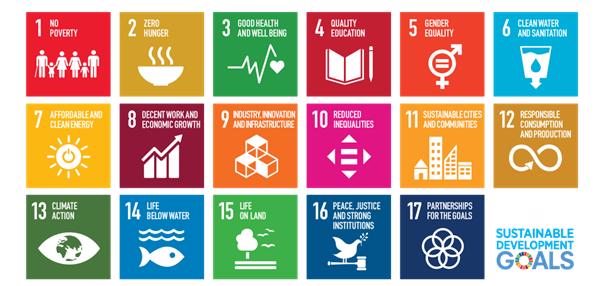
\includegraphics[width=0.7\textwidth]{Figures/Picture1}
    \caption[The seventeen UN Sustainable Development Goals; KhetLens targets Goals 2 and 12.]{The seventeen United Nations Sustainable Development Goals, shown as a grid of coloured tiles each with a number, a short title and an icon: 1 No Poverty, 2 Zero Hunger, 3 Good Health and Well-being, 4 Quality Education, 5 Gender Equality, 6 Clean Water and Sanitation, 7 Affordable and Clean Energy, 8 Decent Work and Economic Growth, 9 Industry, Innovation and Infrastructure, 10 Reduced Inequalities, 11 Sustainable Cities and Communities, 12 Responsible Consumption and Production, 13 Climate Action, 14 Life Below Water, 15 Life on Land, 16 Peace, Justice and Strong Institutions, 17 Partnerships for the Goals. KhetLens targets Goal 2 primarily and Goal 12 secondarily.}
    \label{fig:sdg}
\end{figure}

\section{Constraints}
\label{sec:constraints}
\begin{itemize}
  \item \textbf{Target hardware.} The app must run on entry-level Android phones with about 3\,GB of RAM and Android 8.1 or later, using the CPU only.
  \item \textbf{Connectivity.} All farmer-facing functions must work without a network; the network is used only when available and never blocks the farmer.
  \item \textbf{Storage.} The model, content and audio must fit comfortably on a low-cost phone; we are targeting a model under 10\,MB and a total install under 150\,MB.
  \item \textbf{Data.} Field photographs from Punjab depend on seasonal field visits with our partner; public datasets from other regions are used alongside them.
  \item \textbf{Language resources.} We record the Urdu and Punjabi audio ourselves so that terminology and pronunciation can be checked by the agronomists.
  \item \textbf{Content.} Treatment guidance must be consistent with Pakistan's pesticide regulations and provincial advisories and reviewed by an agronomist before release.
  \item \textbf{Privacy.} Photographs and precise location stay on the phone unless the farmer chooses to share them; only the district is stored on the server.
  \item \textbf{Academic.} Two semesters, three students, and limited GPU time through Colab, Kaggle and the university's GPU server.
\end{itemize}

\section{Business Opportunity}
Our immediate route to farmers is our industry partner. Fatima Fertiliser has a nationwide network of dealers and field officers through which KhetLens can be demonstrated and supported, and its agronomists give the treatment content a credibility that a student application could not establish alone. For the partner, an offline diagnosis tool strengthens its relationship with farmers and, through the feedback loop, yields district-level disease-incidence information that the partner does not currently have.

Beyond the partnership, the design (a swappable model, a class list and a content pack) allows the application to be adapted for other agricultural companies, seed suppliers and provincial extension departments, and extended to further crops. Aggregated incidence data would be of interest to research institutes and the Pest Warning service. The best-known commercial comparator, Plantix~\cite{plantix}, performs its diagnosis online and is used mainly in India; KhetLens's offline operation, Punjabi and Urdu support, locally reviewed guidance and honest handling of uncertainty are its differentiation.

\section{Stakeholders Description / User Characteristics}
Six groups have a stake in KhetLens. Table~\ref{tab:stakeholders} describes each and its role, and Table~\ref{tab:stakeholder-goals} summarises the goals and current problems of those who interact with the system directly.

\subsection{Stakeholders Summary}
\begin{table}[H]
\centering\small
\caption{Stakeholders of KhetLens.}
\label{tab:stakeholders}
\begin{tabularx}{\textwidth}{|L{3.2cm}|Y|L{3.2cm}|}
\hline
\textbf{Stakeholder} & \textbf{Description} & \textbf{Role} \\ \hline
Farmer & Grows wheat, maize or cotton in Punjab; speaks Punjabi, may read Urdu; owns an entry-level Android phone with intermittent connectivity. & Primary user \\ \hline
Partner agronomists & Plant protection specialists at Fatima Fertiliser; review the disease list, treatment content and follow-up questions. & Domain expert, reviewer \\ \hline
Partner field officers & Visit farms regularly; can install and demonstrate the app and support photograph collection and feedback. & Distribution, data collection \\ \hline
Project team & Three BS(CS) students; design, build, train, test and document the system; maintain the content. & Developer, administrator \\ \hline
Supervisor and FYP panel & Faculty of the FAST School of Computing. & Academic oversight \\ \hline
Punjab Agriculture Department & Publishes advisories and approved-product lists. & Content source \\ \hline
\end{tabularx}
\end{table}

\subsection{Key High-Level Goals and Problems of Stakeholders}
\begin{table}[H]
\centering\small
\caption{Goals and problems of the main stakeholders.}
\label{tab:stakeholder-goals}
\begin{tabularx}{\textwidth}{|L{3.0cm}|Y|Y|}
\hline
\textbf{Stakeholder} & \textbf{Goals} & \textbf{Current problems} \\ \hline
Farmer & Know quickly what is wrong and what to do; avoid wasting money on the wrong treatment; understand the answer in their own language. & No expert nearby; dealer advice may be biased; existing apps need internet and English. \\ \hline
Agronomist & Give correct, compliant advice at scale; know which diseases are appearing where. & Too few to visit every farm; advice is diluted before it reaches the farmer. \\ \hline
Field officer & Serve more farmers per visit with a credible tool. & No diagnostic support in the field; paper records. \\ \hline
Project team & Deliver a working, evaluated system in two semesters and answer the research questions. & Field data depends on the season; limited GPU time; low-end hardware. \\ \hline
\end{tabularx}
\end{table}

\section{Conclusion}
This chapter has framed KhetLens as a practical answer to a well-known gap: disease classifiers that work in the laboratory but are not available to the farmer in a form that fits their phone, language and need for honest advice. We have broken the problem into four parts, set nine objectives, drawn the boundary of the scope, and identified the constraints and stakeholders that shape the design. The next chapter reviews the research and applications our approach builds on.

\chapter{Literature Review / Related Work}
\label{ch:lit}

Our design draws on five areas of prior work: how image-based plant disease classifiers behave on field photographs and the datasets built for that setting; compact neural networks and their compression for phones; methods for detecting out-of-distribution inputs and calibrating confidence; the use of environmental context in diagnosis; and the data efficiency of transfer and few-shot learning. We also review the main deployed applications and the regional work on our three crops. For each work we summarise what was done, note its strengths and limitations, and state how it relates to KhetLens. A summary table closes the chapter.

\section{Definitions, Acronyms, and Abbreviations}
In addition to the terms in Section~\ref{sec:acronyms}: \textbf{in-distribution} data resembles the training data, while \textbf{out-of-distribution} (OOD) data does not; \textbf{open-set recognition} is classification with an explicit ``unknown'' outcome; \textbf{domain shift} is the change in image statistics between training and deployment, here between laboratory and field photographs; a \textbf{learning curve} plots accuracy against the number of training examples; \textbf{late fusion} combines the outputs of separate models or signals.

\section{Detailed Literature Review}
The review is organised into six categories that follow the sub-problems of Chapter~\ref{ch:vision}.

\subsection{Field conditions and field datasets}
\label{sec:lit-gap}
\textbf{Hughes and Salath\'e~\cite{hughes2015plantvillage}; Mohanty et al.~\cite{mohanty2016}.} PlantVillage released over 54,000 leaf images of 14 crops and 38 classes photographed against plain backgrounds, and Mohanty et al.\ trained standard CNNs on it to 99.35\% held-out accuracy. The paper also reported a sharp drop when the model was applied to images from other sources. \emph{Analysis:} the dataset's scale launched the research area, and its uniform style is also its main limitation. \emph{Relation to our work:} PlantVillage provides our maize classes and a pre-training corpus; its limitation is why we evaluate only on field photographs.

\textbf{Noyan~\cite{noyan2022bias}; Xu et al.~\cite{xu2024datasets}.} Noyan showed that a classifier trained on only a few background pixels of PlantVillage images still performs far above chance, revealing a background--label correlation. Xu et al.\ surveyed around forty public datasets and found that most were built for benchmarking rather than for realistic deployment, with large accuracy differences between laboratory and field variants. \emph{Analysis:} both are careful studies of dataset bias; Xu et al.\ also note that even expert labellers disagree on some wheat images. \emph{Relation:} they motivate our background-aware augmentation and our use of field-only test sets.

\textbf{Singh et al.~\cite{singh2020plantdoc}; Wei et al.~\cite{wei2024plantwild}; Ahmad et al.~\cite{ahmad2021cds}.} PlantDoc provides about 2,600 field images across 13 species, and fine-tuning on it instead of PlantVillage improved field accuracy by up to 31 percentage points. PlantWild, with over 18,000 in-the-wild images and 89 classes, is the largest public field benchmark. CD\&S provides over 4,000 field images of three maize diseases with severity labels. \emph{Analysis:} these datasets show that accuracy on field images is substantially lower than on laboratory images even for strong models, and that mixed-source training helps. \emph{Relation:} PlantDoc and CD\&S supply maize field images for KhetLens, and PlantWild is used for plant-domain pre-training.

\textbf{FieldPlant and the controlled-versus-field generalisation study~\cite{fieldplant2023,gen2023fieldcond}.} Both works build dedicated field datasets and measure how models trained under controlled conditions perform on them; the generalisation study finds that adding field images to training and removing backgrounds both improve field performance. \emph{Analysis:} they are the most direct measurements of the question our first research question asks. \emph{Relation:} they justify our mixed-source training, background augmentation and field-only test set.

\subsection{Compact on-device models and compression}
\label{sec:lit-mobile}
\textbf{Howard et al.~\cite{howard2019mnv3}.} MobileNetV3 combines hardware-aware architecture search with efficient building blocks and has well-documented latency on mobile CPUs. \emph{Analysis:} it remains the most practical family for CPU-only phones, while newer hybrid transformer designs trade some latency for accuracy. \emph{Relation:} MobileNetV3-Large is our deployed model, with a smaller MobileNetV3 and a hybrid as benchmarked alternatives.

\textbf{Kumar et al.~\cite{kumar2025benchmark}; Tonmoy et al.~\cite{tonmoy2025mobileplantvit}; Khan et al.~\cite{khan2023edge}.} Kumar et al.\ benchmarked mobile CNNs on over 76,000 images and 101 classes, finding MobileNetV3-Large at 92.6\% with a 21.6\,MB float model and EfficientNet-B1 at 94.7\% with a larger model. MobilePlantViT, a hybrid with under one million parameters, generalised well across datasets of very different sizes. Khan et al.\ quantised MobileNetV3-Small to 8-bit integers with under one million parameters and no accuracy loss on PlantVillage. \emph{Analysis:} together these give a clear accuracy-versus-size picture across the architectures we are choosing between, though they report desktop rather than phone latency. \emph{Relation:} they support MobileNetV3-Large as a good balance and motivate our own on-phone measurements.

\textbf{Hinton et al.~\cite{hinton2015kd}; Krishnamoorthi~\cite{krishnamoorthi2018quant}.} Knowledge distillation trains a small student on a larger teacher's softened outputs, typically recovering a few points of accuracy; the quantisation whitepaper shows that calibrated post-training quantisation stays within about 2\% of floating point and quantisation-aware training within about 1\%. \emph{Analysis:} these are the standard, well-tested recipes for shipping a small accurate model. \emph{Relation:} KhetLens distils its student from a larger teacher and uses quantisation-aware training with a calibration set that includes field images.

\textbf{Zhang et al.~\cite{zhangq2022mobilebench}; Ramcharan et al.~\cite{ramcharan2019cassava}.} A benchmark of mobile inference libraries across ten phones found large latency differences between libraries for the same model, and INT8 speed-ups on CPU that vary widely. Ramcharan et al.\ ran a MobileNet detector for cassava diseases on a budget Android phone and evaluated it on real-world images, where accuracy was lower than on the test set and lowest for mild symptoms. \emph{Analysis:} both show that performance has to be measured on the target device and on real photographs rather than assumed. \emph{Relation:} we benchmark our runtime options on entry-level phones and evaluate on field photographs.

\subsection{Out-of-distribution detection and calibration}
\label{sec:lit-ood}
\textbf{Hendrycks and Gimpel~\cite{hendrycks2017msp}; Guo et al.~\cite{guo2017calibration}.} The maximum softmax probability is the baseline OOD score, and a single temperature parameter fitted on validation data restores calibration at no inference cost. \emph{Analysis:} simple and widely reproduced. \emph{Relation:} we report the softmax baseline for every OOD result and apply temperature scaling to all deployed confidences.

\textbf{Lee et al.~\cite{lee2018mahalanobis}; Sun et al.~\cite{sun2021react}; Liu et al.~\cite{liu2020energy}.} The Mahalanobis detector scores inputs by their distance to class-conditional Gaussians in feature space; ReAct clips unusually high activations and improves most detectors; the energy score replaces softmax with the log-sum-exp of the logits. \emph{Analysis:} all are inexpensive at inference and need only a few stored statistics, which suits a phone; all are weaker on inputs that are semantically close to the training classes. \emph{Relation:} our novelty check uses a Mahalanobis distance on clipped features, and we compare energy with the softmax baseline for the unknown-disease check.

\textbf{Fuentes et al.~\cite{fuentes2021openset}; Meng et al.~\cite{meng2023osr}.} Open-set recognition has been applied to tomato disease, where a model trained on one domain had to recognise unknown classes in another~\cite{fuentes2021openset}, and to multi-dataset plant recognition, where plant-domain pre-training and a margin-based loss tightened the known classes and improved unknown detection~\cite{meng2023osr}. \emph{Analysis:} these establish that the classification loss and pre-training matter for unknown detection, not only the score. \emph{Relation:} we adopt a margin-based loss and calibrate thresholds on field photographs.

\textbf{Erg\"un et al.~\cite{ergun2026grape}.} On grape disease under field conditions, temperature scaling reduced the calibration error of MobileNetV3-Large and EfficientNet-B0 several-fold. \emph{Analysis:} the study uses the same backbones we use and separates calibration from accuracy cleanly. \emph{Relation:} it sets the calibration approach of our uncertainty check.

\textbf{Ahmed et al.~\cite{ahmed2022agropath}.} AgroPath, developed in Lahore, filters blurred, defocused and poorly lit leaf photographs before classification with a small quality-assessment model and reports high accuracy on the photographs it retains. \emph{Analysis:} it shows that an image-quality gate is practical in a field setting. \emph{Relation:} it is the basis of the quality stage of our uncertainty check.

\textbf{Mrisho et al.~\cite{mrisho2020nuru}; Sottocornola et al.~\cite{sottocornola2022dssapple}.} The field validation of PlantVillage Nuru in East Africa found that photographing several leaves per plant raised accuracy substantially over a single leaf, and that the app compared well with extension officers and farmers. DSSApple diagnoses post-harvest apple disease through rounds of picture-based questions. \emph{Analysis:} both show that simple interaction, more photographs or a few picture questions, is an effective way to reduce uncertainty. \emph{Relation:} they are the basis of our ``take more photos'' and follow-up question steps.

\subsection{Context-aware diagnosis}
\label{sec:lit-context}
\textbf{Picon et al.~\cite{picon2019cropcond}.} A crop-conditional CNN trained on more than 100,000 smartphone field images of five crops, including wheat and maize, raised balanced accuracy from 0.93 to 0.98 by injecting the crop identity into the network. \emph{Analysis:} the clearest demonstration that cheap metadata improves field diagnosis, on a proprietary dataset. \emph{Relation:} our shared backbone with a crop head and per-crop disease heads follows this design.

\textbf{Xu and Wang~\cite{xuwang2025fusion}.} A recent wheat study fused image features with temperature, humidity and soil-moisture readings and reported high accuracy on three classes from a small dataset. \emph{Analysis:} weather carries signal, but learned fusion needs large paired datasets to be reliable, and missing context must be handled explicitly. \emph{Relation:} these are the reasons we fuse weather through a rule-based prior that falls back gracefully when weather is unavailable.

\textbf{Ali et al.~\cite{ali2023striperust}; Ahmad et al.~\cite{ahmad2018clcuv}.} A regression model fitted on five years of data from Layyah, Punjab, predicts stripe rust severity from temperature, rainfall and humidity and identifies the conducive ranges; a Pakistani model of cotton leaf curl relates disease intensity to humidity, rainfall and whitefly populations. \emph{Analysis:} regional epidemiological studies that quantify exactly the weather--disease relationships we need. \emph{Relation:} they supply the ranges in our weather plausibility table.

\subsection{Data efficiency}
\label{sec:lit-data}
\textbf{Beck et al.~\cite{beck2022curves}.} Accuracy on crop images follows a power law in training-set size, and label noise flattens the curve. \textbf{Argüeso et al.~\cite{argueso2020fewshot}; Xu et al.~\cite{xu2022transfer}.} A Siamese few-shot network reached about 80\% with 15 images per class and 90\% with 80; a transformer pre-trained on millions of plant images reached much higher few-shot accuracy than an ImageNet model. \emph{Analysis:} these provide comparable shot grids and the functional form for a learning curve. \emph{Relation:} our field-data study uses a matching ladder of images per class and fits the same curve, and plant-domain pre-training is one of our benchmarked options.

\subsection{Work on wheat, maize and cotton in the region}
\label{sec:lit-region}
\textbf{Wheat.} The NWRD dataset from NUST provides pixel-level rust annotations on Pakistani wheat~\cite{anwar2023nwrd}; Malik and Hayat classified wheat leaves into five classes, including both rusts and powdery mildew, from phone photographs collected in Punjab and KP~\cite{malik2025wheatpk}; Long et al.\ classified five wheat conditions from a large set of field and glasshouse images and released a public test subset~\cite{long2024ukwheat}. \emph{Relation:} together these cover our wheat classes and show that phone capture in Punjab works well.

\textbf{Maize.} Published work on maize converges on the three leaf diseases we cover, common rust, northern leaf blight and grey leaf spot, which between them are covered by PlantVillage, PlantDoc and CD\&S~\cite{hughes2015plantvillage,singh2020plantdoc,ahmad2021cds}. \emph{Relation:} this confirms the class set we use for maize.

\textbf{Cotton.} Anwar et al.\ trained transfer-learning models on a mix of Pakistani field and online images of healthy, bacterial blight and leaf curl leaves~\cite{anwarcotton2023pk}; Ahmad et al.\ staged leaf curl severity in Bahawalpur and Multan from RGB and multispectral images~\cite{ahmad2024clcuvfusion}; the CoSEV dataset provides Pakistani field photographs with severity stages~\cite{noon2023cosev}; SAR-CLD-2024 provides over two thousand field photographs of seven cotton conditions~\cite{sarcld2024}; and Wang et al.\ built a compact cotton network on an eleven-class dataset~\cite{wang2025cotton}. \emph{Relation:} these supply all six of our cotton classes.

\section{Application Review}
\label{sec:apps}
\textbf{Plantix~\cite{plantix}.} The most widely used commercial crop-diagnosis app, covering many crops and diseases with a community forum and product suggestions, used mainly in India. \emph{Strengths:} breadth, polish, large user base. \emph{Limitations:} diagnosis is performed online; languages and products target the Indian market. \emph{Relevance:} the benchmark for breadth and user experience; KhetLens differentiates on offline operation, Pakistani languages and uncertainty handling.

\textbf{PlantVillage Nuru~\cite{mrisho2020nuru}.} An offline object-detection app for cassava diseases validated in the field in East Africa, where it compared favourably with extension officers and farmers and benefited from photographing several leaves. \emph{Strengths:} offline, field-validated. \emph{Limitations:} one crop; weaker on mild symptoms. \emph{Relevance:} the closest precedent for KhetLens and the source of our multi-photo step.

\textbf{Offline prototypes~\cite{offlinemnv3app2026}.} Recent conference work describes offline mobile prototypes built on MobileNetV3 and TensorFlow Lite. \emph{Relevance:} they confirm that the engineering path we follow is practical; of the prototypes we reviewed, none combines context fusion with uncertainty handling or targets Urdu and Punjabi.

\section{Literature Review Summary Table}
\label{sec:littable}
Table~\ref{tab:litsummary} summarises the research literature in the format required for research projects, and Table~\ref{tab:appsummary} the applications.

\small
\begin{longtable}{|L{2.6cm}|L{4.0cm}|L{4.2cm}|L{3.4cm}|}
\caption{Summary of research literature reviewed.}
\label{tab:litsummary}\\
\hline
\textbf{Author} & \textbf{Method} & \textbf{Results} & \textbf{Limitations} \\ \hline
\endfirsthead
\multicolumn{4}{l}{\small\textit{Table \thetable\ continued}}\\ \hline
\textbf{Author} & \textbf{Method} & \textbf{Results} & \textbf{Limitations} \\ \hline
\endhead
\hline \multicolumn{4}{r}{\small\textit{continued on next page}} \\
\endfoot
\hline
\endlastfoot
Mohanty et al.~\cite{mohanty2016} & CNNs on PlantVillage, 38 classes & 99.35\% held-out accuracy & Laboratory images only \\ \hline
Noyan~\cite{noyan2022bias} & Classifier on background pixels & Far above chance; background bias & One dataset \\ \hline
Xu et al.~\cite{xu2024datasets} & Survey of $\sim$40 datasets & Large lab-to-field differences & Review; second-hand figures \\ \hline
Singh et al.~\cite{singh2020plantdoc} & PlantDoc field dataset; PV pre-train, PD fine-tune & Up to +31 points field accuracy & Small; web-scraped \\ \hline
Wei et al.~\cite{wei2024plantwild} & PlantWild, 18,542 wild images, 89 classes & Best baseline 67.2\% & Web-sourced \\ \hline
Ahmad et al.~\cite{ahmad2021cds} & CD\&S maize field dataset with severity & 4,455 images & Three diseases \\ \hline
Howard et al.~\cite{howard2019mnv3} & MobileNetV3 architecture search & Best latency--accuracy on mobile CPUs & General, not agri \\ \hline
Kumar et al.~\cite{kumar2025benchmark} & Mobile CNN benchmark, 101 classes & MNv3-L 92.6\%; EffNet-B1 94.7\% & No phone latency \\ \hline
Tonmoy et al.~\cite{tonmoy2025mobileplantvit} & Sub-1M hybrid ViT & Generalises across datasets of different sizes & No device data \\ \hline
Khan et al.~\cite{khan2023edge} & MNv3-Small, INT8, ONNX & 99.5\% PV; $<$1M params & Desktop CPU \\ \hline
Hinton et al.~\cite{hinton2015kd} & Knowledge distillation & Student recovers most of the teacher's accuracy & General \\ \hline
Krishnamoorthi~\cite{krishnamoorthi2018quant} & PTQ and QAT whitepaper & PTQ within 2\%, QAT within 1\% & General \\ \hline
Zhang et al.~\cite{zhangq2022mobilebench} & Mobile DL library benchmark, 10 phones & Large library-dependent latency differences & 2022 versions \\ \hline
Ramcharan et al.~\cite{ramcharan2019cassava} & MobileNet detector on a budget phone & Real-world accuracy below test set & One crop \\ \hline
Hendrycks \& Gimpel~\cite{hendrycks2017msp} & Softmax baseline for OOD & Baseline across tasks & Over-confident \\ \hline
Guo et al.~\cite{guo2017calibration} & Temperature scaling & Restores calibration & Not domain shift \\ \hline
Lee et al.~\cite{lee2018mahalanobis} & Mahalanobis on features & Needs only class statistics & Gaussian assumption \\ \hline
Sun et al.~\cite{sun2021react} & ReAct activation clipping & Large FPR reduction & Clipping level must be chosen \\ \hline
Liu et al.~\cite{liu2020energy} & Energy score & Beats softmax & Threshold tuning \\ \hline
Meng et al.~\cite{meng2023osr} & Plant open-set recognition & AUROC 93.7 & Heavy backbone \\ \hline
Erg\"un et al.~\cite{ergun2026grape} & Calibration of MNv3-L / EffNet-B0, field grape & Several-fold ECE reduction & One crop \\ \hline
Ahmed et al.~\cite{ahmed2022agropath} & Image-quality gate before classification & Higher accuracy on retained images & Post-filter figure \\ \hline
Mrisho et al.~\cite{mrisho2020nuru} & Field validation of Nuru, East Africa & Multi-leaf capture raises accuracy & Small sample \\ \hline
Picon et al.~\cite{picon2019cropcond} & Crop-conditional CNN, 5 crops & Balanced acc.\ 0.93 $\to$ 0.98 & Proprietary data \\ \hline
Xu \& Wang~\cite{xuwang2025fusion} & Image + sensor fusion, wheat & High accuracy on 3 classes & Small dataset \\ \hline
Ali et al.~\cite{ali2023striperust} & Weather regression of stripe rust, Layyah & $R^2$ 90.7\%; conducive ranges & Region-specific \\ \hline
Ahmad et al.~\cite{ahmad2018clcuv} & CLCuV vs weather, Pakistan & Humidity, rain, whitefly drive intensity & Monthly resolution \\ \hline
Beck et al.~\cite{beck2022curves} & Learning curves on crop images & Power law; noise flattens curve & Species, not disease \\ \hline
Argüeso et al.~\cite{argueso2020fewshot} & Siamese few-shot & 80\% @15, 90\% @80 per class & Not field images \\ \hline
Xu et al.~\cite{xu2022transfer} & Plant-domain pre-trained ViT, few-shot & 86.3\% @20-shot & Not edge-friendly \\ \hline
Malik \& Hayat~\cite{malik2025wheatpk} & CNNs on Punjab/KP wheat phone photos & 95\% & Small original set \\ \hline
Anwar et al.~\cite{anwarcotton2023pk} & Transfer learning, Pakistani cotton & 96\% at 256 px & Two diseases \\ \hline
Ahmad et al.~\cite{ahmad2024clcuvfusion} & RGB + multispectral CLCuV severity & RGB 81\%; fused 96\% & Needs extra sensor \\ \hline
Long et al.~\cite{long2024ukwheat} & CNNs on 19k wheat field/glasshouse images & 97.1\%; public test set & Different climate \\ \hline
Wang et al.~\cite{wang2025cotton} & Compact cotton network, 11 classes & 98.4\%; 4.8 MB & Random split; no separate field test \\ \hline
\end{longtable}
\normalsize

\begin{table}[H]
\centering\small
\caption{Summary of related applications.}
\label{tab:appsummary}
\begin{tabularx}{\textwidth}{|L{2.6cm}|Y|Y|Y|}
\hline
\textbf{Application} & \textbf{Features} & \textbf{Relevance} & \textbf{Limitations} \\ \hline
Plantix~\cite{plantix} & Multi-crop photo diagnosis, community, product links & Breadth and UX benchmark & Online diagnosis; Indian-market languages \\ \hline
PlantVillage Nuru~\cite{mrisho2020nuru} & Offline cassava detection & Field-validated offline precedent & One crop; weak on mild symptoms \\ \hline
Offline MobileNetV3 prototype~\cite{offlinemnv3app2026} & On-device classification & Same engineering path & Single crop set; no context or uncertainty handling \\ \hline
\end{tabularx}
\end{table}

\section{Conclusion}
\label{sec:gaps}
The literature gives us a solid foundation for each part of KhetLens: field datasets and training practices that generalise beyond the laboratory, compact architectures and compression recipes that run on phones, inexpensive uncertainty measures, regional weather--disease relationships, and interaction patterns that farmers have been shown to use. It also shows where our project adds value. The existing offline prototypes address one part of the problem at a time; KhetLens brings on-device inference, weather context and uncertainty handling together for three crops. Weather has been used in learned fusion with large datasets; we use it as a rule-based prior that needs no paired data and can be reviewed by agronomists. Learning curves have been measured on laboratory sets; we measure them on field photographs for our crops. And the field validation of farmer-facing apps remains rare; we plan ours with our industry partner. The next chapter turns these findings into requirements.

\chapter{Software Requirement Specifications}
\label{ch:srs}

This chapter specifies what KhetLens must do and how well. It lists the features, the functional and non-functional requirements, the assumptions, the use cases in the department's tabular format, the hardware and software needed, the user interface, the database design and the risks. Requirement identifiers (F, FR, NFR, UC, R) are used in the following chapters and will be the basis of the traceability matrix in the implementation report.

\section{List of Features}
\label{sec:features}
\begin{description}[style=nextline, leftmargin=0pt, itemsep=2pt]
  \item[F1 Offline plant-photo diagnosis.] Identify the crop and one of 17 conditions from a photograph of the plant, close up or from a short distance, on the device.
  \item[F2 Capture with live quality feedback.] Real-time blur and exposure warnings before the shutter is pressed, and a quality check after it.
  \item[F3 Weather-aware result.] Adjust the image result using the recent weather of the farmer's district.
  \item[F4 Three-state outcome.] Every diagnosis ends as \emph{Confident}, \emph{Likely} (follow-up questions) or \emph{Unsure} (no guess).
  \item[F5 Picture-based follow-up questions.] Up to three questions, answered by tapping illustrated options.
  \item[F6 Explained result.] Each result shows the reasons behind it and lets the farmer correct the detected crop.
  \item[F7 Treatment guidance.] Treatment and prevention steps per condition, with source and reviewer shown, in three languages with audio.
  \item[F8 Offline disease library.] Reference for all 17 conditions: symptoms, causes, management, audio.
  \item[F9 Diagnosis history.] Diagnoses stored automatically and kept for six months.
  \item[F10 Farmer feedback.] Correctness and treatment-outcome feedback, captured offline, sent when connected and then removed from the phone.
  \item[F11 Three-language interface with audio.] English, Urdu and Punjabi text with recorded audio on every content screen.
  \item[F12 Sign-in with guest mode.] Phone-number sign-in with a one-time code over WhatsApp; diagnosis never requires an account.
  \item[F13 Background updates.] Weather refresh, feedback upload and model or content updates whenever the phone is connected.
\end{description}

\section{Functional Requirements}
\label{sec:fr}
\subsection{Onboarding and account}
\begin{itemize}
  \item \textbf{FR-01} On first launch the system shall offer English, Urdu and Punjabi, each with an audio button that speaks the language name; the choice shall be changeable in Settings. (Farmer)
  \item \textbf{FR-02} The system shall allow sign-in by mobile number: it sends a one-time code over WhatsApp, verifies it, and keeps the farmer signed in while offline. (Farmer)
  \item \textbf{FR-03} The system shall offer ``Skip for now''; in guest mode all diagnosis, library and history functions work, and only feedback upload waits for sign-in. (Farmer)
  \item \textbf{FR-04} The system shall request location permission once, derive the farmer's district on the device, display it, and allow it to be changed manually. (Farmer)
\end{itemize}
\subsection{Capture and diagnosis}
\begin{itemize}
  \item \textbf{FR-05} The system shall provide a camera screen with brief guidance and shall also accept an image from the gallery. (Farmer)
  \item \textbf{FR-06} While the viewfinder is open the system shall show a live warning when the preview is blurred or badly exposed. (Farmer)
  \item \textbf{FR-07} After capture the system shall check the photograph for blur and exposure; if it fails, the system shall show the reason and ask for a retake without running the classifier. (System)
  \item \textbf{FR-08} The system shall identify the crop and show it on the result screen with a one-tap correction; if crop confidence is low it shall ask the farmer to confirm the crop first. (System, Farmer)
  \item \textbf{FR-09} The system shall classify the photograph into one of the conditions of the detected crop, on the device and without network access, whether it is a close-up of a leaf or a wider shot of the plant; wider shots are analysed as a whole and in regions, and the results combined. (System)
  \item \textbf{FR-10} The system shall adjust the class probabilities using the stored weather of the district when a recent snapshot exists; otherwise it shall use the image result alone and say so. (System)
  \item \textbf{FR-11} The system shall compute a novelty score and a calibrated confidence for every diagnosis and assign one of three outcomes: Confident, Likely or Unsure. (System)
  \item \textbf{FR-12} For a Confident outcome the system shall show the condition name, the confidence, a ``Disease confirmed'' or ``Healthy'' badge and at least two reasons. (System)
  \item \textbf{FR-13} For a Likely outcome the system shall ask up to three picture-based questions from the crop's question set and finalise as Confident or Unsure; ``Not sure'' shall be an option for every question. (Farmer)
  \item \textbf{FR-14} For an Unsure outcome the system shall state that nothing was guessed, give the reason, offer to take two more photographs, and offer a field-officer contact; no treatment shall be shown. (System)
\end{itemize}
\subsection{Guidance, library and audio}
\begin{itemize}
  \item \textbf{FR-15} For a Confident result the system shall show treatment and prevention guidance with a safety note, the source and the reviewing agronomist, in the selected language. (Farmer)
  \item \textbf{FR-16} Guidance shall name approved product types and refer to label doses; specific doses appear only where approved by the reviewer. (Content)
  \item \textbf{FR-17} The system shall provide a library of all 17 conditions, filterable by crop, each with symptoms, causes, management and audio, fully offline. (Farmer)
  \item \textbf{FR-18} Every content screen shall have a speaker button that plays recorded audio in the selected language. (Farmer)
\end{itemize}
\subsection{History and feedback}
\begin{itemize}
  \item \textbf{FR-19} The system shall store every completed diagnosis automatically with its photograph, result, confidence and weather snapshot, and shall clear entries older than six months. (System)
  \item \textbf{FR-20} The system shall list recent diagnoses and open any of them to show the full result and guidance. (Farmer)
  \item \textbf{FR-21} The system shall let the farmer record whether a diagnosis was correct and whether the treatment worked, with an optional comment, store it locally and queue it for upload. (Farmer)
  \item \textbf{FR-22} Sharing a photograph with feedback shall be an explicit opt-in; by default photographs do not leave the device. (Farmer)
\end{itemize}
\subsection{Connectivity, updates and backend}
\begin{itemize}
  \item \textbf{FR-23} When connected, the system shall fetch the recent weather (daily temperature, humidity and rainfall over the last two weeks) for the district and store it; the home screen shall show a summary and its age. (System)
  \item \textbf{FR-24} When connected, the system shall upload queued feedback, delete the local copy once the server acknowledges it, and retry later on failure. (System)
  \item \textbf{FR-25} When connected, the system shall check for a newer model or content pack, download it in the background, verify it and switch to it; a failed download shall leave the current version in use. (System)
  \item \textbf{FR-26} The application package shall include a baseline model and content pack so that every function works on first launch. (System)
  \item \textbf{FR-27} The server shall provide endpoints for code request and verification, feedback ingestion, and model and content distribution, and shall store feedback without the farmer's name. (Server)
  \item \textbf{FR-28} The team shall publish new content or models through a tool that validates the content, checks that every guidance entry has a source and reviewer, and records the version. (Team)
\end{itemize}

\section{Quality Attributes}
\label{sec:qa}
In order of priority: \textbf{availability offline} (every farmer-facing function works with no network); \textbf{performance on entry-level hardware}; \textbf{trustworthiness} (calibrated confidence, honest abstention, explained results, attributed guidance); \textbf{usability for low-literacy users} (icon-first, one-handed, audio everywhere, large type, high contrast); \textbf{privacy} (photographs and precise location stay on the device unless shared deliberately); \textbf{maintainability} (model and content updatable without a release); and \textbf{robustness} (sensible behaviour on missing weather, failed downloads and interrupted connectivity).

\section{Non-Functional Requirements}
\label{sec:nfr}
{\small
\begin{longtable}{|L{1.3cm}|L{2.4cm}|L{7.5cm}|L{3.0cm}|}
\caption{Non-functional requirements.}\label{tab:nfr}\\
\hline
\textbf{ID} & \textbf{Category} & \textbf{Requirement} & \textbf{Verification} \\ \hline
\endfirsthead
\multicolumn{4}{l}{\small\textit{Table \thetable\ continued}}\\ \hline
\textbf{ID} & \textbf{Category} & \textbf{Requirement} & \textbf{Verification} \\ \hline
\endhead
\hline \multicolumn{4}{r}{\small\textit{continued on next page}}\\
\endfoot
\endlastfoot
NFR-01 & Performance & A diagnosis is returned within about two seconds on an entry-level Android phone using the CPU only; app start-up within a few seconds. & Measurement on target phones \\ \hline
NFR-02 & Resource use & Model under 10\,MB; content pack with audio under 60\,MB; total install under 150\,MB. & Build artefacts \\ \hline
NFR-03 & Availability & All farmer-facing use cases pass with the network disabled. & Test cases in airplane mode \\ \hline
NFR-04 & Accuracy & Accuracy and macro-F1 reported on a held-out set of field photographs for every model release, with a release target of macro-F1 of 0.80 or higher. & Evaluation report \\ \hline
NFR-05 & Trustworthiness & Calibration error kept low through temperature scaling; unsupported inputs rejected at a high rate while keeping accuracy on supported classes; blurred photographs reliably sent for retake. & Evaluation report \\ \hline
NFR-06 & Usability & Home to treatment in at most four taps; tap targets of at least 48\,dp; body text of at least 16\,sp; checked with farmers through our partner. & UI audit; farmer test \\ \hline
NFR-07 & Localisation & All strings, library entries and guidance available in the three languages, with correct right-to-left layout and Nastaliq rendering and audio on every content screen. & Content audit \\ \hline
NFR-08 & Privacy & Photographs and GPS coordinates never sent without opt-in; only the district stored on the server; sign-in tokens stored in encrypted storage; all traffic over TLS. & Code review \\ \hline
NFR-09 & Reliability & No data loss if the app is closed during a diagnosis or feedback entry; a failed update never leaves the app without a working model. & Fault-injection tests \\ \hline
NFR-10 & Compatibility & Android 8.1 and later; no dependency on a GPU or neural accelerator for core functions. & Device tests \\ \hline
\end{longtable}
}

\section{Assumptions}
\label{sec:assumptions}
\begin{itemize}
  \item Farmers have access to an Android phone meeting NFR-10 with a working camera and about 1\,GB of free storage.
  \item Phones connect to a network at least occasionally, which is enough for weather refresh, feedback upload and updates.
  \item Farmers who sign in have WhatsApp on the same number; those who do not can use guest mode.
  \item Our partner's agronomists review the disease list, treatment content and follow-up questions, and field officers support photograph collection during the growing seasons.
  \item Public datasets are used under their published terms; each source's licence is recorded when it is added.
  \item A free weather service is sufficient for the request volumes involved; the weather module is isolated so another provider can be substituted.
  \item Treatment content is advisory; the farmer and the agronomist remain responsible for product selection and dosing.
\end{itemize}

\section{Use Cases}
\label{sec:usecases}
Figure~\ref{fig:usecase} shows the use-case model. UC-01 to UC-12 belong to the farmer, UC-13 and UC-14 are system-initiated, and UC-15 and UC-16 belong to the team and the agronomist. Each is specified below in the department's format.

\begin{figure}[H]
  \centering
  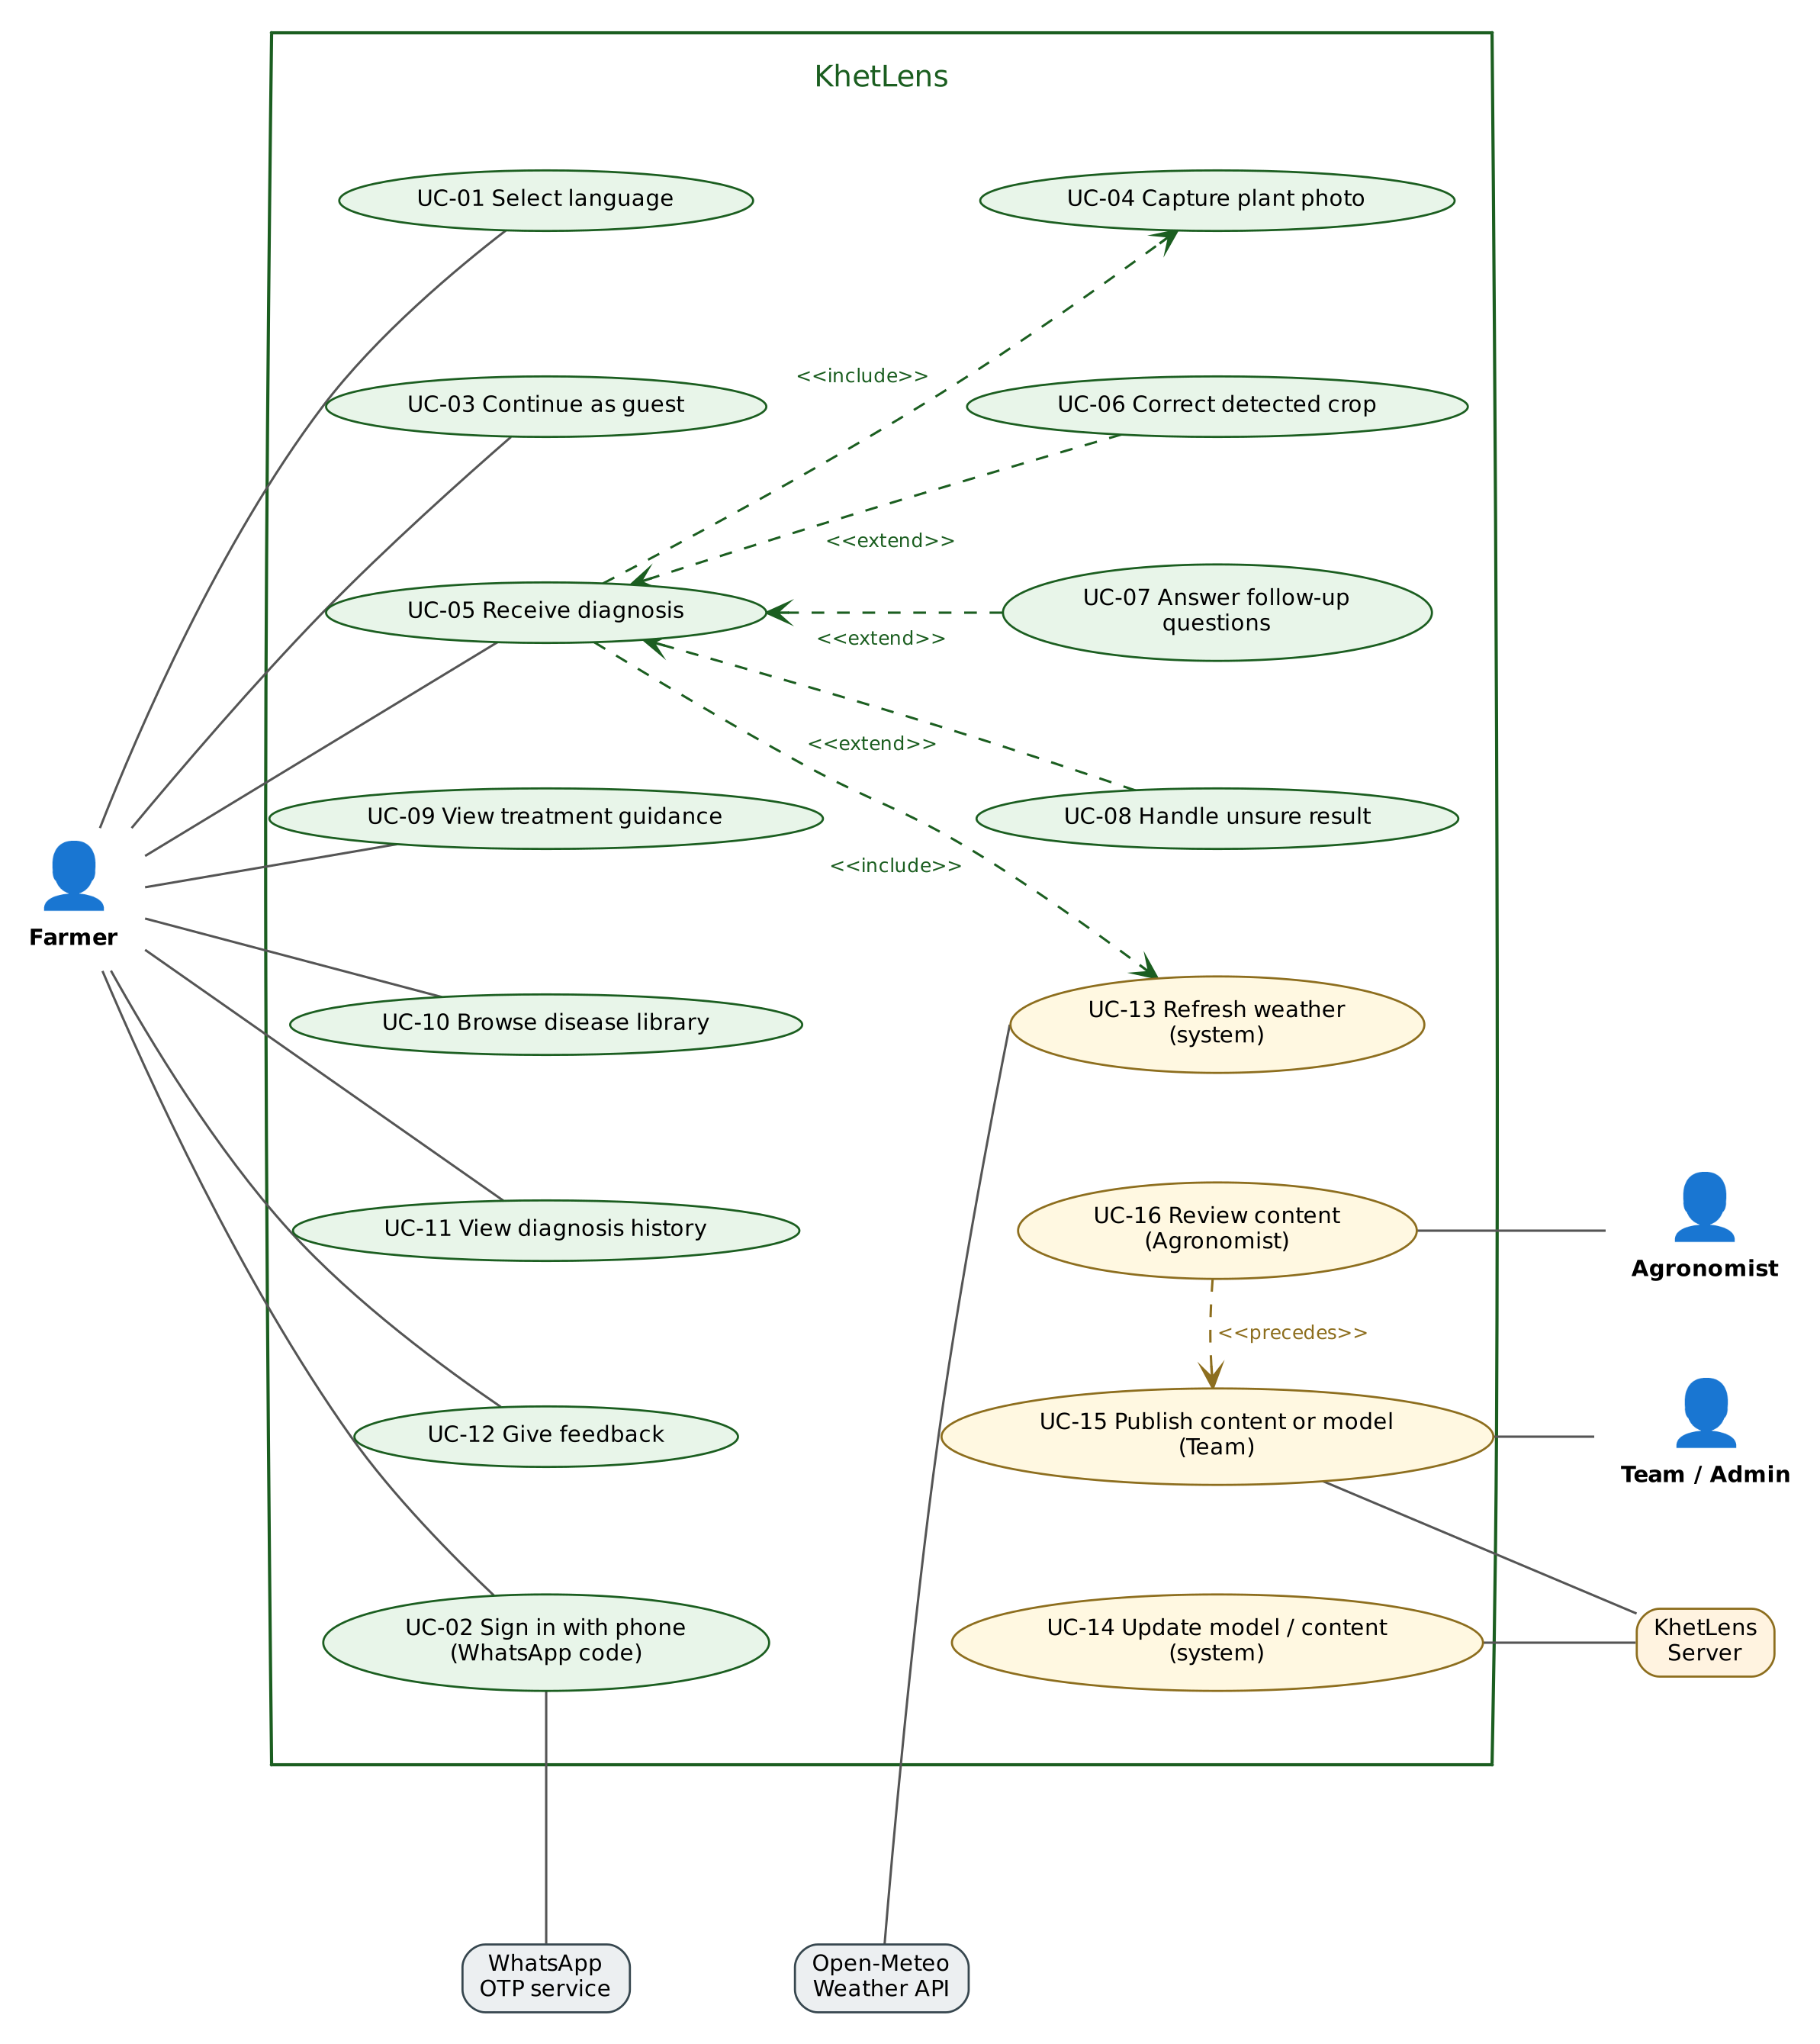
\includegraphics[width=\textwidth,height=0.88\textheight,keepaspectratio]{Figures/diagrams/usecase.png}
  \caption{Use-case diagram of KhetLens.}
  \label{fig:usecase}
\end{figure}

\begin{usecase}{UC-01 Select language}{uc:01}
\ucrow{Name}{Select language}
\ucrow{Actors}{Farmer}
\ucrow{Summary}{The farmer chooses English, Urdu or Punjabi on first launch or from Settings; the interface, library and audio switch to that language.}
\ucrow{Pre-Conditions}{Application installed and opened.}
\ucrow{Post-Conditions}{Language preference saved; all screens rendered in that language.}
\ucrow{Special Requirements}{Each option has a speaker button so that a non-reader can choose.}
\ucflow{Basic Flow}
\ucstep{1. Farmer opens the app for the first time.}{2. System shows three language tiles with speaker icons.}
\ucstep{3. Farmer taps a tile and Continue.}{4. System saves the preference and opens the sign-in screen.}
\ucflow{Alternative Flow}
\ucstep{1a. Farmer opens Settings later and taps Language.}{2a. System shows the same tiles and re-renders the current screen on selection.}
\ucstep{3a. Farmer taps a speaker icon first.}{4a. System plays the language name aloud and waits.}
\end{usecase}

\begin{usecase}{UC-02 Sign in with phone (WhatsApp code)}{uc:02}
\ucrow{Name}{Sign in with phone number}
\ucrow{Actors}{Farmer; WhatsApp OTP service}
\ucrow{Summary}{The farmer enters a mobile number, receives a one-time code on WhatsApp, enters it and stays signed in.}
\ucrow{Pre-Conditions}{Phone connected to a network; language selected.}
\ucrow{Post-Conditions}{Sign-in token stored; feedback upload enabled.}
\ucrow{Special Requirements}{Code requests limited per number; sign-in is optional (UC-03).}
\ucflow{Basic Flow}
\ucstep{1. Farmer enters the mobile number and taps Send code on WhatsApp.}{2. System asks the server to send a code and shows the code entry field.}
\ucstep{3. Farmer enters the 6-digit code.}{4. System verifies it with the server, stores the token and opens Home.}
\ucflow{Alternative Flow}
\ucstep{1a. Farmer is offline.}{2a. System explains that sign-in needs a connection and offers Skip for now.}
\ucstep{3a. Farmer enters a wrong or expired code.}{4a. System shows an error and offers to resend after a short wait.}
\end{usecase}

\begin{usecase}{UC-03 Continue as guest}{uc:03}
\ucrow{Name}{Continue as guest}
\ucrow{Actors}{Farmer}
\ucrow{Summary}{The farmer skips sign-in and uses all diagnostic functions without an account.}
\ucrow{Pre-Conditions}{Language selected.}
\ucrow{Post-Conditions}{Guest profile created; feedback is stored but not uploaded until sign-in.}
\ucrow{Special Requirements}{The sign-in prompt is shown only when the farmer tries to send feedback.}
\ucflow{Basic Flow}
\ucstep{1. Farmer taps ``Skip for now''.}{2. System creates a guest profile and opens Home.}
\ucflow{Alternative Flow}
\ucstep{1a. Guest later taps Send feedback.}{2a. System saves the feedback locally and offers sign-in to enable upload.}
\end{usecase}

\begin{usecase}{UC-04 Capture plant photo}{uc:04}
\ucrow{Name}{Capture plant photo}
\ucrow{Actors}{Farmer}
\ucrow{Summary}{The farmer photographs the affected plant, close up or from a short distance, with live blur and exposure feedback; the photograph is quality-checked before diagnosis.}
\ucrow{Pre-Conditions}{Camera permission granted; Home screen open.}
\ucrow{Post-Conditions}{A photograph that passed the check is handed to UC-05; otherwise the farmer is asked to retake.}
\ucrow{Special Requirements}{Live indicator updates smoothly; the quality check adds no noticeable delay.}
\ucflow{Basic Flow}
\ucstep{1. Farmer taps ``Diagnose a plant''.}{2. System opens the camera with the guidance ``Point at the affected plant, hold steady''.}
\ucstep{3. Farmer points the camera at the plant or at a leaf.}{4. System shows a live indicator: green when sharp and well lit, amber when blurred or dark.}
\ucstep{5. Farmer presses the shutter.}{6. System checks blur and exposure and, on pass, continues to UC-05.}
\ucflow{Alternative Flow}
\ucstep{5a. Farmer taps Gallery and picks an image.}{6a. System runs the same check on the chosen image.}
\ucstep{5b. Farmer's photograph is blurred or dark.}{6b. System shows the reason (too blurry, too dark) and returns to the viewfinder.}
\end{usecase}

\begin{usecase}{UC-05 Receive diagnosis}{uc:05}
\ucrow{Name}{Receive diagnosis}
\ucrow{Actors}{Farmer}
\ucrow{Summary}{The system identifies the crop and condition on the device, applies the weather adjustment and the uncertainty check, and shows a Confident, Likely or Unsure outcome.}
\ucrow{Pre-Conditions}{Photograph passed the quality check; model loaded.}
\ucrow{Post-Conditions}{Diagnosis saved in history with outcome, probabilities and weather snapshot.}
\ucrow{Special Requirements}{No network access; uses the stored weather if it is recent (FR-10).}
\ucflow{Basic Flow}
\ucstep{1. Farmer waits after pressing the shutter.}{2. System runs the model: crop head, then the disease head of the detected crop.}
\ucstep{3. Farmer sees the progress indicator.}{4. System computes novelty and confidence, applies the weather prior and assigns the outcome.}
\ucstep{5. Farmer views the result screen.}{6. System shows crop, condition, confidence, badge, the ``Not [crop]?'' chip and the Why panel, and saves the record.}
\ucstep{7. Farmer taps ``See treatment''.}{8. System opens UC-09.}
\ucflow{Alternative Flow}
\ucstep{5a. Farmer sees a crop-confirmation prompt (crop confidence low).}{6a. System shows three crop tiles and continues with the chosen crop (UC-06).}
\ucstep{5b. Farmer sees a Likely result.}{6b. System opens the follow-up questions (UC-07).}
\ucstep{5c. Farmer sees an Unsure result.}{6c. System opens the unsure screen (UC-08).}
\ucstep{5d. Farmer diagnoses with no recent weather stored.}{6d. System uses the image result alone and notes ``Weather context unavailable''.}
\end{usecase}

\begin{usecase}{UC-06 Correct detected crop}{uc:06}
\ucrow{Name}{Correct detected crop}
\ucrow{Actors}{Farmer}
\ucrow{Summary}{The farmer overrides the detected crop; the system re-runs the disease head for the chosen crop.}
\ucrow{Pre-Conditions}{A result is shown, or the system has asked for crop confirmation.}
\ucrow{Post-Conditions}{Record updated with the corrected crop and a correction flag.}
\ucrow{Special Requirements}{Re-inference is immediate.}
\ucflow{Basic Flow}
\ucstep{1. Farmer taps ``Not wheat?'' on the result screen.}{2. System shows three crop tiles.}
\ucstep{3. Farmer taps the correct crop.}{4. System re-runs the disease head for that crop and refreshes the result.}
\ucflow{Alternative Flow}
\ucstep{3a. Farmer taps ``None of these''.}{4a. System sets the outcome to Unsure with reason ``crop not supported'' and opens UC-08.}
\end{usecase}

\begin{usecase}{UC-07 Answer follow-up questions}{uc:07}
\ucrow{Name}{Answer follow-up questions}
\ucrow{Actors}{Farmer}
\ucrow{Summary}{When two conditions remain plausible, the system asks up to three picture-based questions and refines the result.}
\ucrow{Pre-Conditions}{Outcome of UC-05 is Likely.}
\ucrow{Post-Conditions}{Outcome finalised as Confident or Unsure; answers saved with the diagnosis.}
\ucrow{Special Requirements}{Questions and pictures come from the reviewed content pack; audio for each question.}
\ucflow{Basic Flow}
\ucstep{1. Farmer reads or listens to the first question.}{2. System shows two or three illustrated options and a progress indicator.}
\ucstep{3. Farmer taps an option.}{4. System updates the result and shows the next question, or finalises as Confident if one condition now dominates.}
\ucflow{Alternative Flow}
\ucstep{3a. Farmer taps ``Not sure''.}{4a. System moves to the next question without changing the result.}
\ucstep{3b. Three questions answered without a clear winner.}{4b. System finalises as Unsure and opens UC-08.}
\end{usecase}

\begin{usecase}{UC-08 Handle unsure result}{uc:08}
\ucrow{Name}{Handle unsure result}
\ucrow{Actors}{Farmer}
\ucrow{Summary}{The system declines to guess, explains why, and offers two more photographs or a field-officer contact.}
\ucrow{Pre-Conditions}{Outcome is Unsure.}
\ucrow{Post-Conditions}{Either a combined result from three photographs or an Unsure record with its reason.}
\ucrow{Special Requirements}{No treatment is shown for an Unsure result (FR-14).}
\ucflow{Basic Flow}
\ucstep{1. Farmer reads ``We're not sure'' and the reason.}{2. System shows ``Nothing was guessed'' and two actions.}
\ucstep{3. Farmer taps ``Take 2 more photos''.}{4. System opens the camera twice, combines the results of all photographs that passed the check, and shows the combined outcome.}
\ucflow{Alternative Flow}
\ucstep{3a. Farmer taps ``Contact field officer''.}{4a. System shows the partner's helpline number.}
\ucstep{3b. Farmer taps Back.}{4b. System saves the Unsure record and returns to Home.}
\end{usecase}

\begin{usecase}{UC-09 View treatment guidance}{uc:09}
\ucrow{Name}{View treatment guidance}
\ucrow{Actors}{Farmer}
\ucrow{Summary}{The farmer reads and listens to treatment and prevention guidance for a confidently diagnosed condition.}
\ucrow{Pre-Conditions}{Confident outcome, or a library entry opened.}
\ucrow{Post-Conditions}{None (read-only).}
\ucrow{Special Requirements}{Source and reviewer shown; audio in the selected language.}
\ucflow{Basic Flow}
\ucstep{1. Farmer taps ``See treatment''.}{2. System shows the Treat and Prevent tabs, numbered steps, a safety note and the attribution.}
\ucstep{3. Farmer taps the speaker button.}{4. System plays the audio for the visible tab.}
\ucflow{Alternative Flow}
\ucstep{3a. Farmer taps Prevent.}{4a. System shows the prevention steps.}
\end{usecase}

\begin{usecase}{UC-10 Browse disease library}{uc:10}
\ucrow{Name}{Browse disease library}
\ucrow{Actors}{Farmer}
\ucrow{Summary}{The farmer browses all supported conditions by crop and opens any for symptoms, causes, management and audio.}
\ucrow{Pre-Conditions}{Content pack installed (bundled with the app).}
\ucrow{Post-Conditions}{None.}
\ucrow{Special Requirements}{Fully offline; names in the selected language with English beneath.}
\ucflow{Basic Flow}
\ucstep{1. Farmer taps Library.}{2. System shows crop filter chips and a grid of condition cards.}
\ucstep{3. Farmer taps a crop chip, then a card.}{4. System filters the grid and opens the entry with its speaker button and treatment link.}
\ucflow{Alternative Flow}
\ucstep{3a. Farmer types in the search field.}{4a. System filters cards by name in any of the three languages.}
\end{usecase}

\begin{usecase}{UC-11 View diagnosis history}{uc:11}
\ucrow{Name}{View diagnosis history}
\ucrow{Actors}{Farmer}
\ucrow{Summary}{The farmer reviews diagnoses from the last six months and reopens any result.}
\ucrow{Pre-Conditions}{At least one recent diagnosis stored.}
\ucrow{Post-Conditions}{None.}
\ucrow{Special Requirements}{Entries older than six months are cleared automatically (FR-19).}
\ucflow{Basic Flow}
\ucstep{1. Farmer taps History.}{2. System lists recent diagnoses with thumbnail, date, crop, condition, outcome colour and feedback status.}
\ucstep{3. Farmer taps an entry.}{4. System shows the stored result with its Why panel, treatment link and feedback status.}
\ucflow{Alternative Flow}
\ucstep{3a. Farmer long-presses an entry and chooses Delete.}{4a. System asks for confirmation and deletes the record and photograph.}
\end{usecase}

\begin{usecase}{UC-12 Give feedback}{uc:12}
\ucrow{Name}{Give feedback}
\ucrow{Actors}{Farmer}
\ucrow{Summary}{The farmer reports whether a diagnosis was correct and whether the treatment worked; the feedback is stored and sent when connected.}
\ucrow{Pre-Conditions}{A diagnosis exists in history.}
\ucrow{Post-Conditions}{Feedback stored locally and queued for upload; removed from the phone after the server acknowledges it (FR-24).}
\ucrow{Special Requirements}{Works offline; large icon options; photo sharing is opt-in.}
\ucflow{Basic Flow}
\ucstep{1. Farmer taps ``Save \& give feedback'' or ``Feedback pending''.}{2. System asks ``Was the diagnosis correct?'' with thumbs up and down.}
\ucstep{3. Farmer taps an option.}{4. System asks ``Did the treatment work?'' with Better, Same and Worse and an optional comment.}
\ucstep{5. Farmer taps Send feedback.}{6. System stores the record, shows ``Saved, sent when you are online'' and schedules the upload; after the server acknowledges it the local copy is deleted.}
\ucflow{Alternative Flow}
\ucstep{3a. Farmer taps thumbs down.}{4a. System also asks ``What was it?'' with the crop's conditions and ``Don't know''.}
\ucstep{5b. Farmer is a guest.}{6b. System saves the record and offers sign-in to enable upload.}
\end{usecase}

\begin{usecase}{UC-13 Refresh weather (system)}{uc:13}
\ucrow{Name}{Refresh weather context}
\ucrow{Actors}{System; weather service}
\ucrow{Summary}{When the phone is connected and the stored weather is more than a day old, the system fetches the last two weeks of district weather and stores it.}
\ucrow{Pre-Conditions}{District known; network available.}
\ucrow{Post-Conditions}{New weather snapshot stored; home-screen chip updated.}
\ucrow{Special Requirements}{Runs in the background; never delays a diagnosis.}
\ucflow{Basic Flow}
\ucstep{1. System detects connectivity and a stale snapshot.}{2. System requests daily temperature, humidity and rainfall for the district for the last 14 days.}
\ucstep{3. System receives the response.}{4. System stores the snapshot with its fetch time and derives the summary used by the weather prior.}
\ucflow{Alternative Flow}
\ucstep{3a. Request fails or times out.}{4a. System keeps the previous snapshot and retries later.}
\end{usecase}

\begin{usecase}{UC-14 Update model / content (system)}{uc:14}
\ucrow{Name}{Update model or content pack}
\ucrow{Actors}{System; KhetLens server}
\ucrow{Summary}{When connected, the system checks for a newer model or content pack, downloads it in the background, verifies it and switches to it.}
\ucrow{Pre-Conditions}{Network available; current versions known.}
\ucrow{Post-Conditions}{New version active; previous version kept until the new one has run successfully.}
\ucrow{Special Requirements}{Checksum verification; atomic switch (FR-25).}
\ucflow{Basic Flow}
\ucstep{1. System contacts the server with its current versions.}{2. Server replies with the latest versions and download links.}
\ucstep{3. System downloads any newer files in the background.}{4. System verifies the checksums, switches to the new files and reloads the model.}
\ucflow{Alternative Flow}
\ucstep{3a. Download is interrupted or the checksum does not match.}{4a. System discards the partial files and keeps the current version.}
\end{usecase}

\begin{usecase}{UC-15 Publish content or model (Team)}{uc:15}
\ucrow{Name}{Publish content pack or model release}
\ucrow{Actors}{Team}
\ucrow{Summary}{The team validates and publishes a reviewed content pack or an evaluated model release to the server.}
\ucrow{Pre-Conditions}{Content reviewed by the agronomist (UC-16) or model evaluated against NFR-04 and NFR-05.}
\ucrow{Post-Conditions}{New version available to the app through UC-14.}
\ucrow{Special Requirements}{The tool rejects guidance entries without source and reviewer and models without a class map and thresholds.}
\ucflow{Basic Flow}
\ucstep{1. Team member runs the publish tool on the pack or model.}{2. Tool validates the content, computes checksums and uploads the files and metadata.}
\ucstep{3. Team member confirms the release.}{4. Server marks the version as current.}
\ucflow{Alternative Flow}
\ucstep{1a. Validation fails.}{2a. Tool lists the problems and stops.}
\end{usecase}

\begin{usecase}{UC-16 Review content (Agronomist)}{uc:16}
\ucrow{Name}{Review content pack}
\ucrow{Actors}{Agronomist}
\ucrow{Summary}{A partner agronomist reviews the disease entries, treatment guidance, weather table and follow-up questions and approves each entry.}
\ucrow{Pre-Conditions}{Draft content exported by the team as a readable review document.}
\ucrow{Post-Conditions}{Each entry carries the reviewer's name and date; unapproved entries are not published.}
\ucrow{Special Requirements}{Review takes place offline on a document; the team records the decisions.}
\ucflow{Basic Flow}
\ucstep{1. Agronomist receives the review document.}{2. Team answers any questions about the format.}
\ucstep{3. Agronomist marks each entry approved or adds comments.}{4. Team updates the content and records the reviewer and date.}
\ucflow{Alternative Flow}
\ucstep{3a. Agronomist proposes a new condition or question.}{4a. Team assesses data availability and schedules it for a later release if feasible.}
\end{usecase}

\section{Hardware and Software Requirements}
\label{sec:hwsw}
The requirements below cover the farmer's device, on which the product must run, and the resources we need to build it.
\subsection{Hardware Requirements}
\begin{itemize}
  \item \textbf{Farmer's device:} an entry-level Android phone with Android 8.1 or later, about 3\,GB of RAM, a rear camera, GPS and about 1\,GB of free storage. We test on entry-level phones available to the team and through our partner.
  \item \textbf{Development:} laptops for Android development and data preparation.
  \item \textbf{Training:} GPU access through Google Colab and Kaggle for iteration, and the university's GPU server for the larger training runs and the field-data study.
  \item \textbf{Server:} a small cloud virtual machine for the backend and database, with object storage for model and content files.
  \item \textbf{Audio:} a USB microphone and a quiet room for recording the Urdu and Punjabi guidance.
\end{itemize}
\subsection{Software Requirements}
\begin{itemize}
  \item \textbf{Mobile:} Kotlin with Jetpack Compose, the Android camera and database libraries, and the TensorFlow Lite (LiteRT) runtime; Android Studio.
  \item \textbf{Training:} Python, PyTorch and timm, ONNX and the TensorFlow Lite converter, scikit-learn, NumPy, pandas and Matplotlib.
  \item \textbf{Backend:} Python with FastAPI, PostgreSQL, Docker.
  \item \textbf{Content:} JSON content pack with a schema; Opus audio; Noto Nastaliq Urdu and Noto Sans fonts.
  \item \textbf{Tooling:} Git and GitHub for source control and issues; LaTeX for documentation.
\end{itemize}

\section{Graphical User Interface}
\label{sec:gui}
We designed the interface for a farmer who may read little, uses the phone one-handed outdoors in bright light, and wants an answer quickly. Every screen follows six rules: a pictogram for each primary action with its label beneath in the selected language; at most two primary actions per screen, the main one a large button at the bottom within thumb reach; a speaker button on every content screen; a four-item bottom navigation (Diagnose, Library, History, Settings); high-contrast colours, with amber reserved for ``likely'' and red only for ``disease confirmed''; and large text with Nastaliq rendering for Urdu and Punjabi. Figure~\ref{fig:nav} shows the navigation flow; the main path from Home to treatment takes four taps. Figures~\ref{fig:gui1} to~\ref{fig:gui4} show the screens, with the use cases each one supports.

\begin{figure}[H]
  \centering
  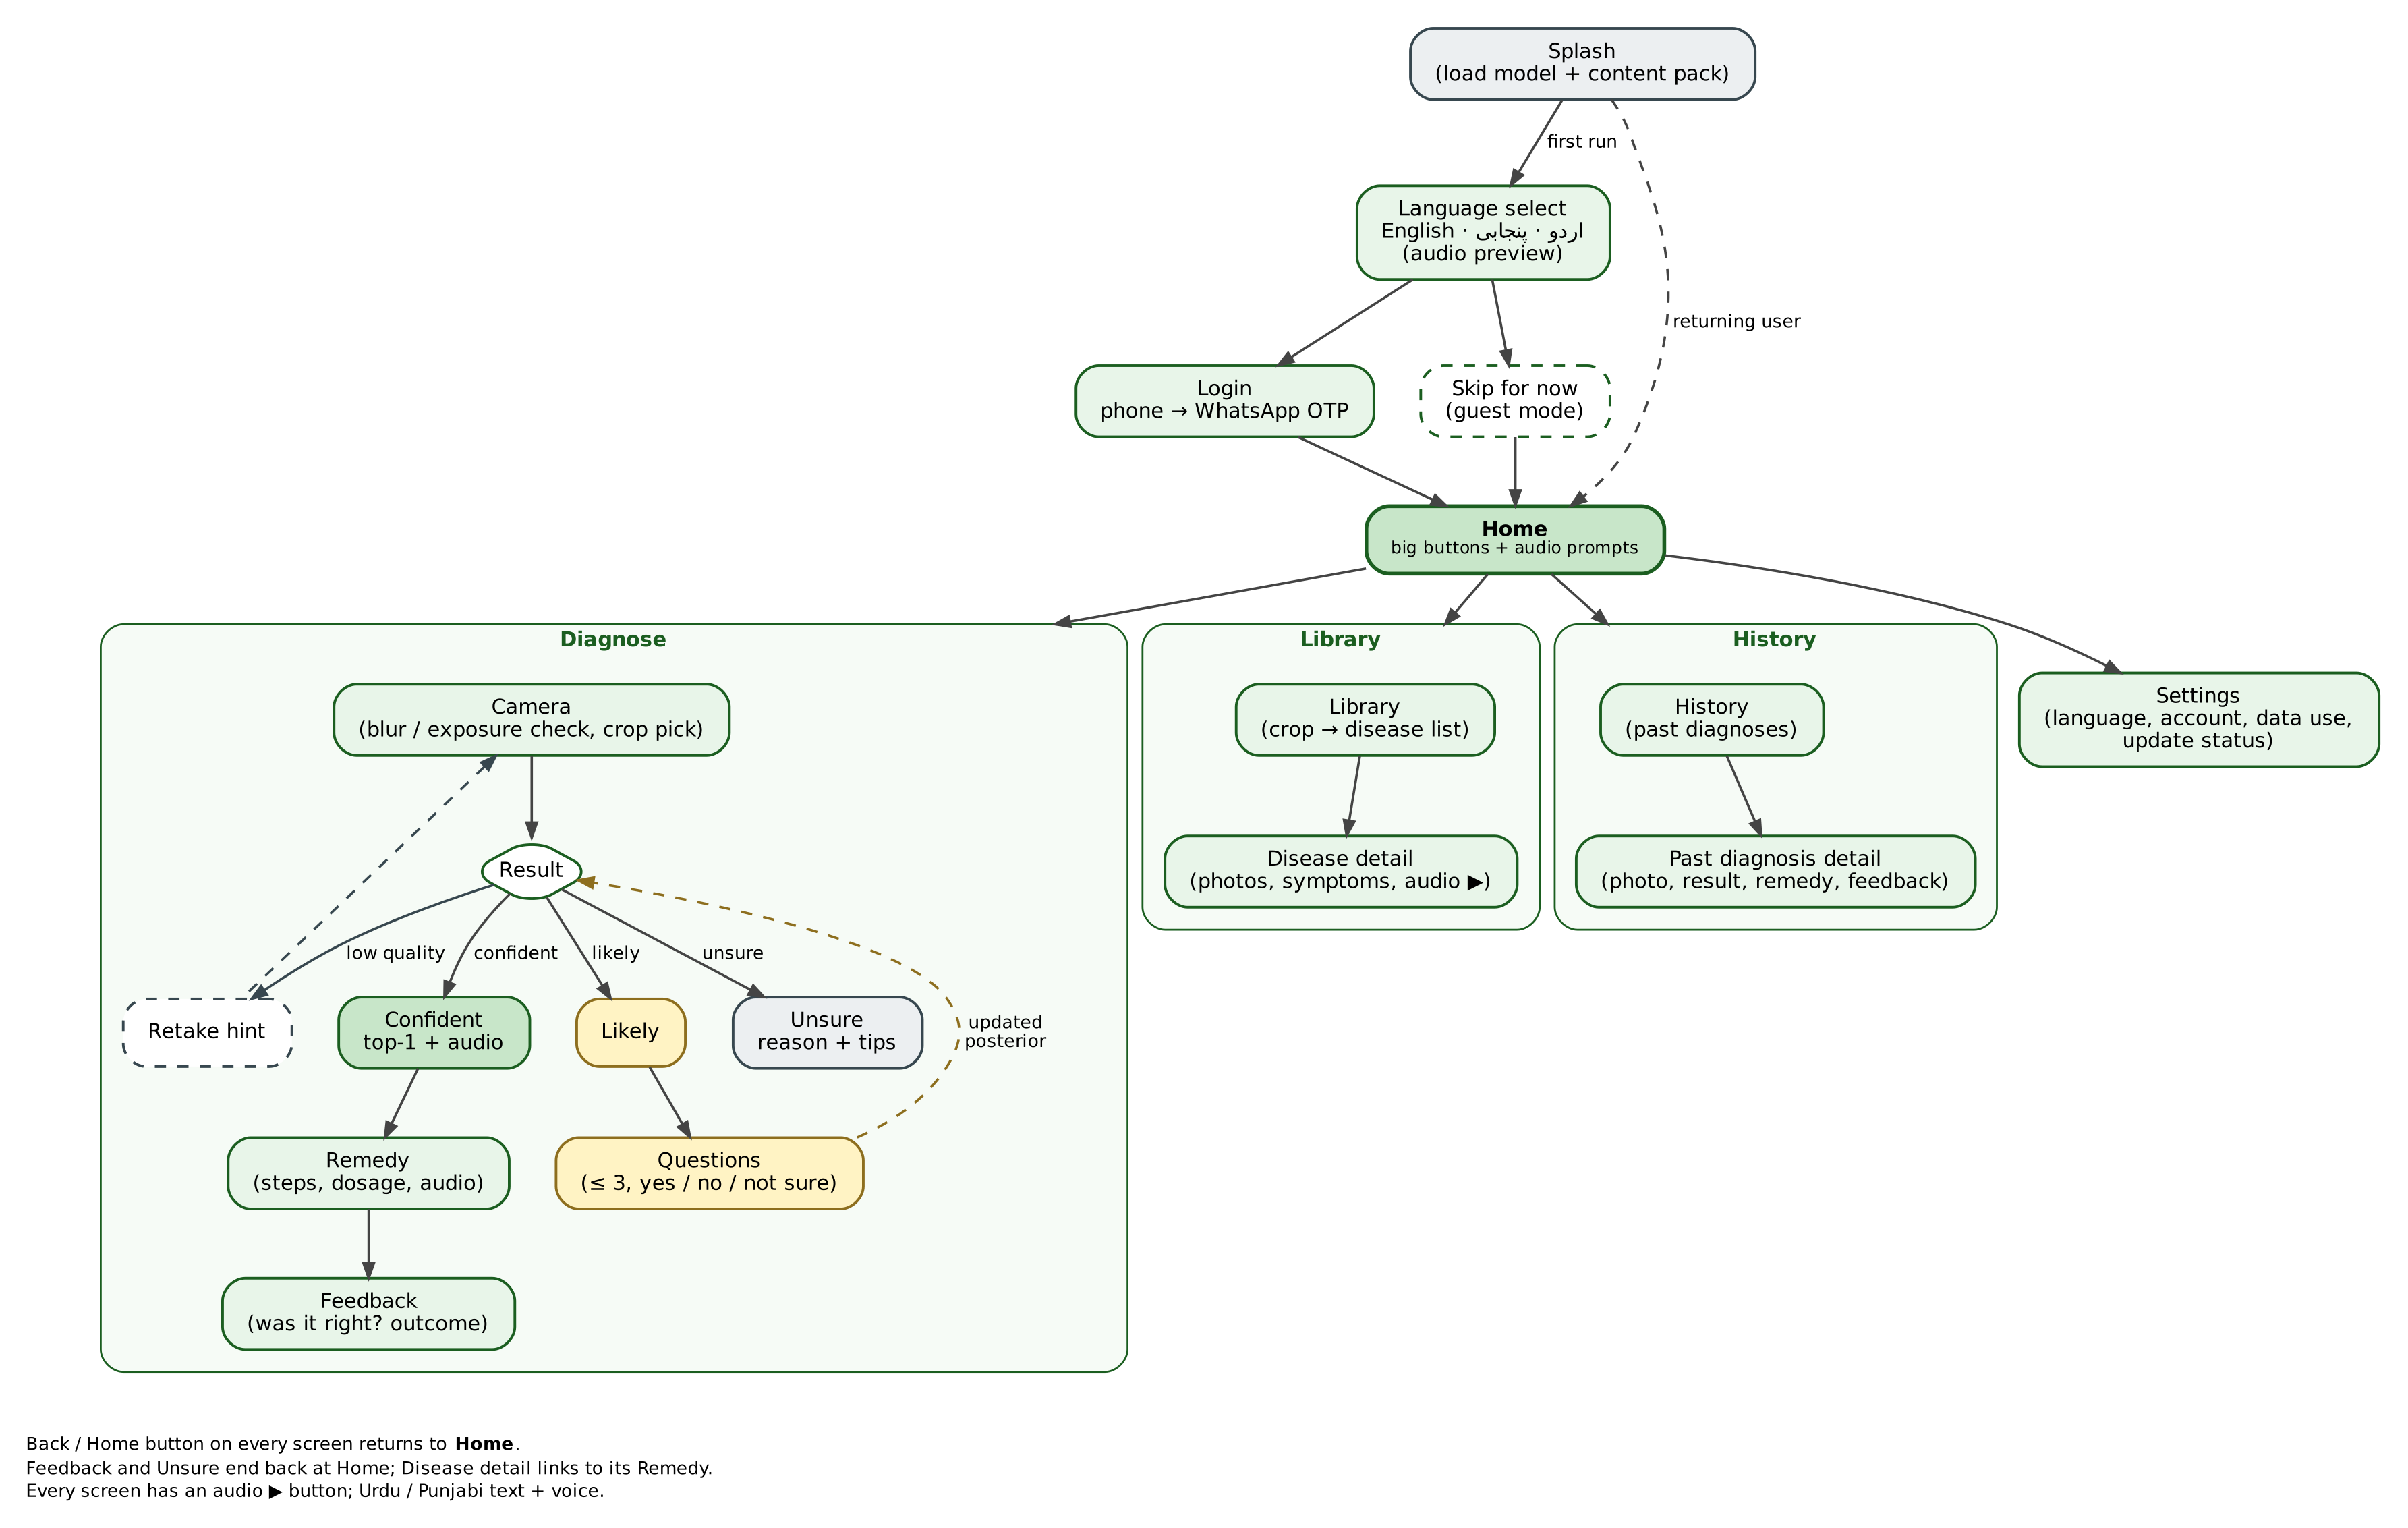
\includegraphics[width=\textwidth,height=0.88\textheight,keepaspectratio]{Figures/diagrams/nav_flow.png}
  \caption{Navigation flow. The primary path Home $\to$ Camera $\to$ Result $\to$ Treatment is four taps; the result branches into Confident, Likely and Unsure states.}
  \label{fig:nav}
\end{figure}

\begin{figure}[H]
  \centering
  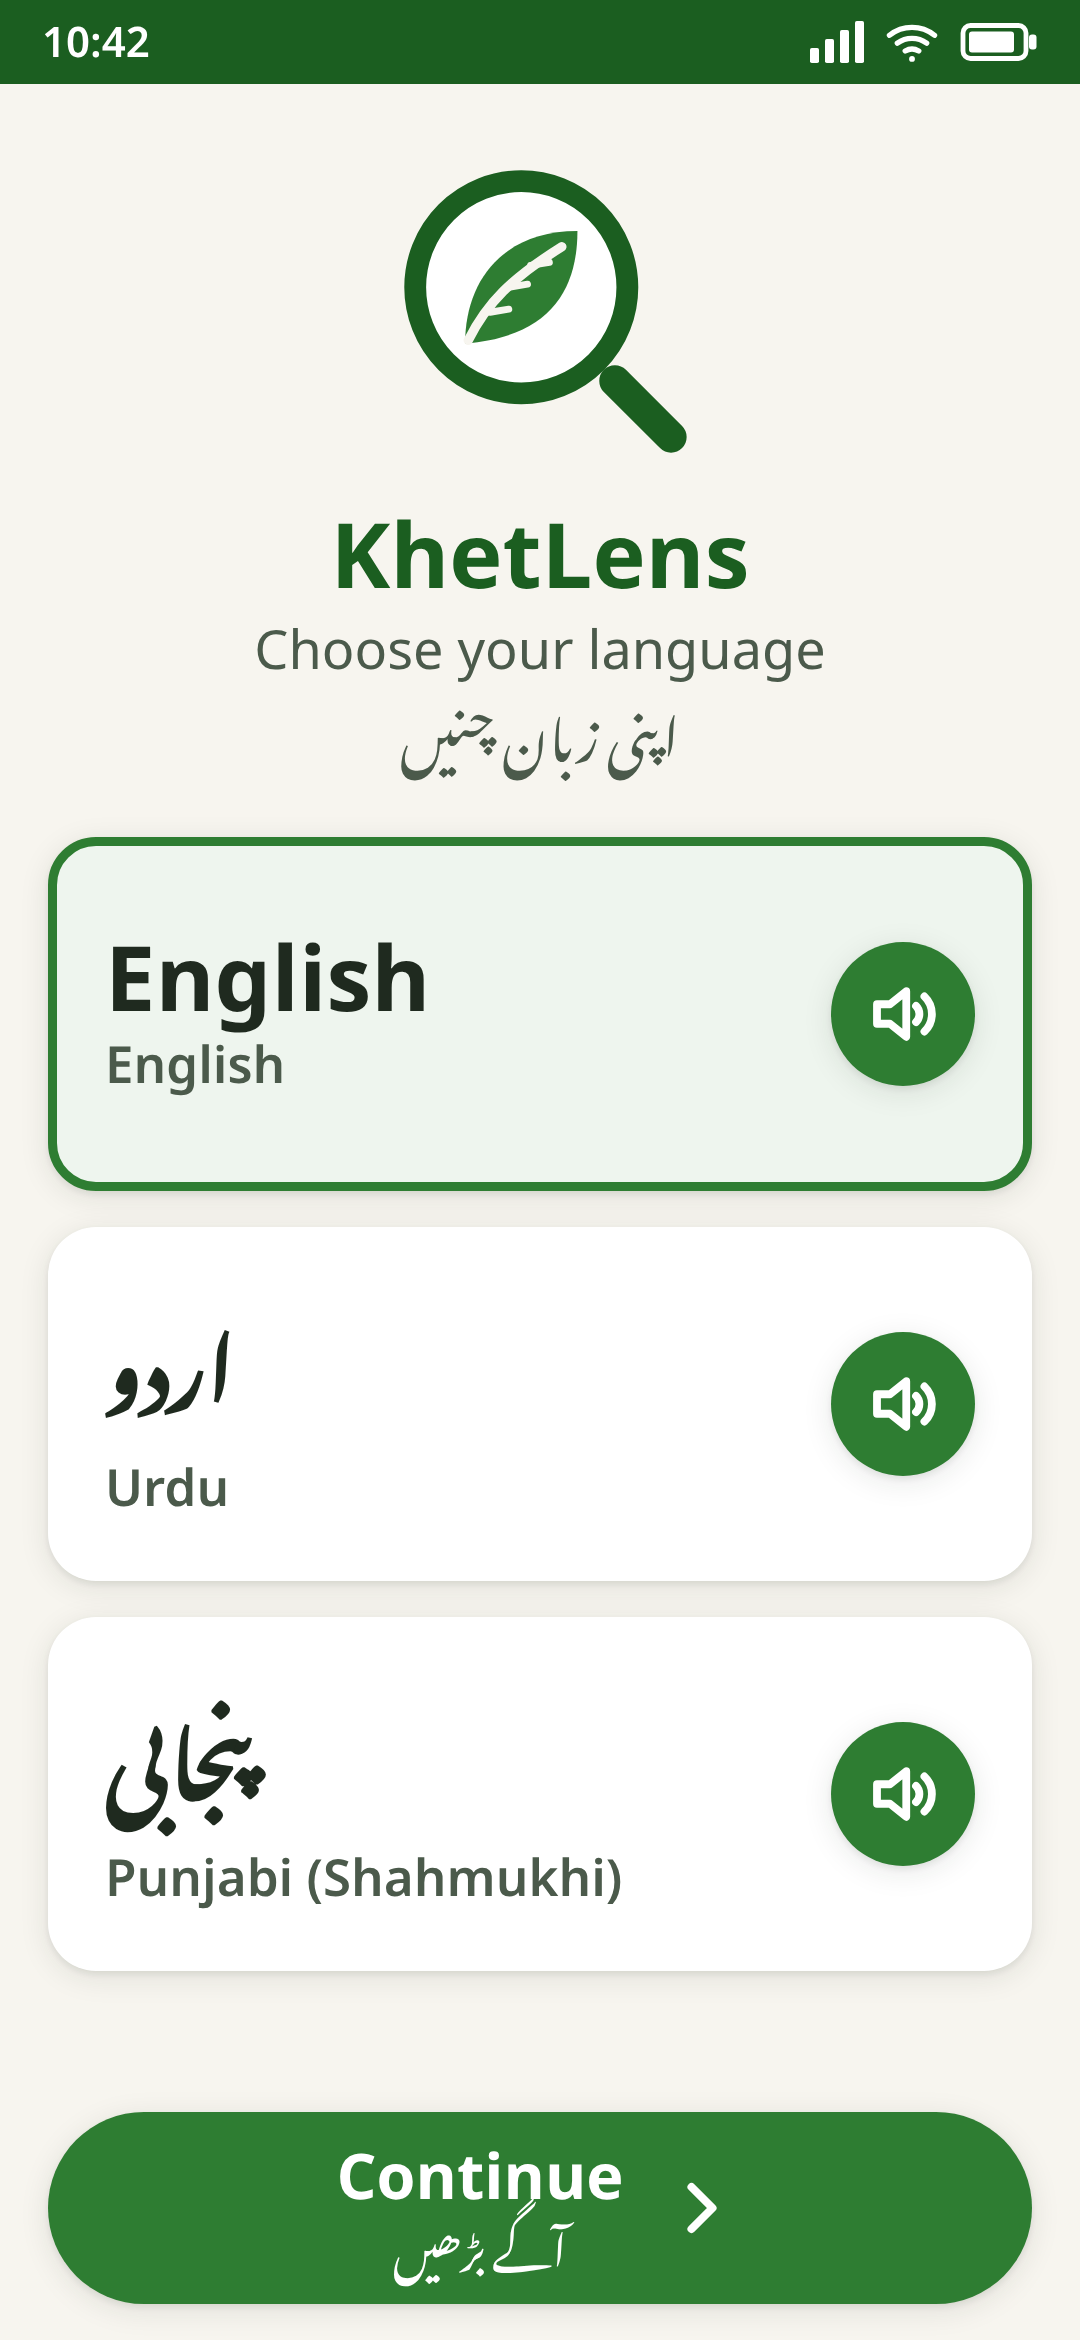
\includegraphics[width=0.3\textwidth]{Figures/gui/01_language.png}\hspace{0.03\textwidth}
  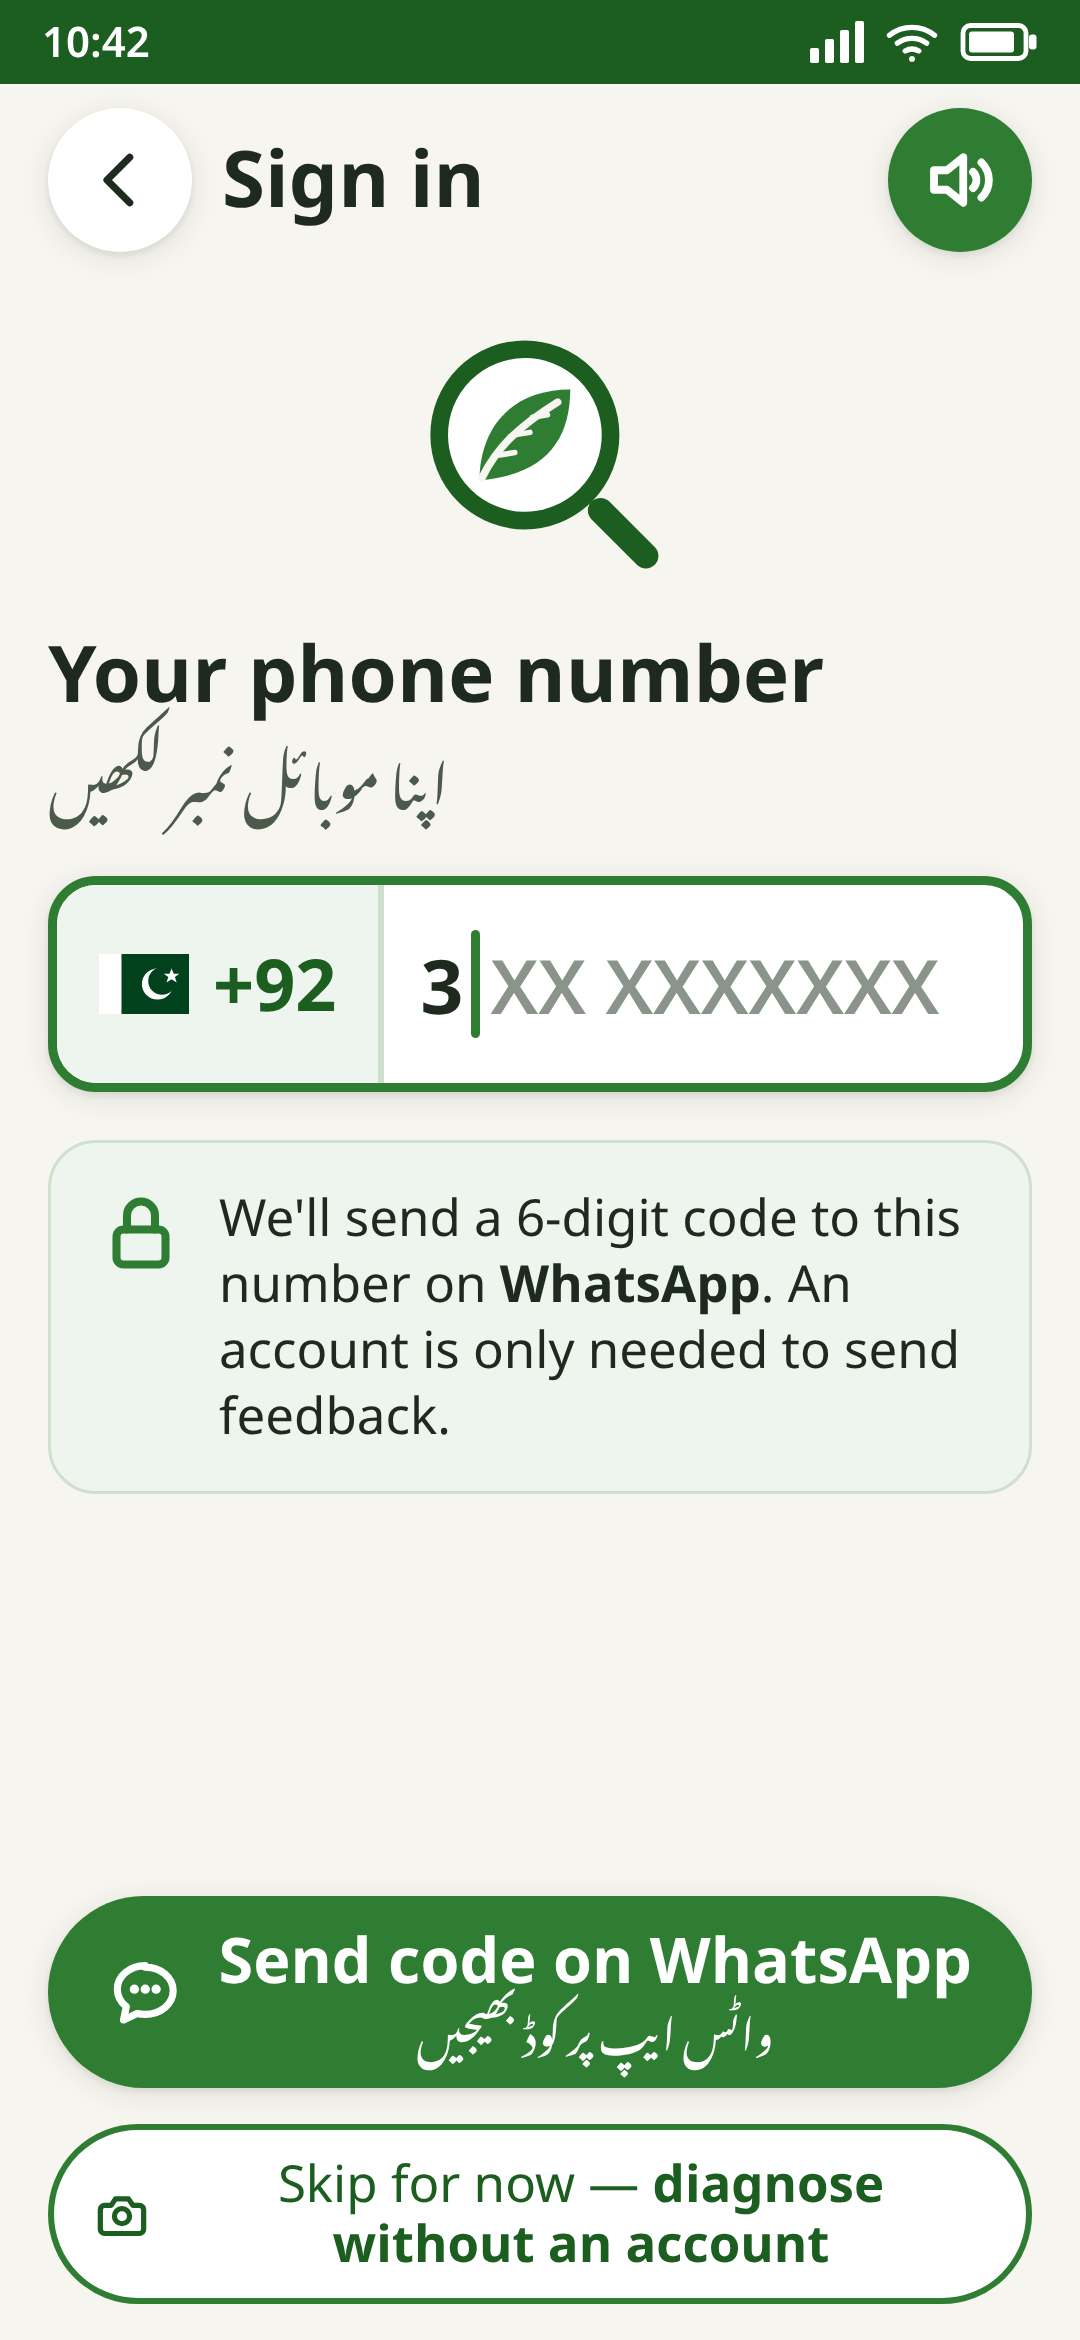
\includegraphics[width=0.3\textwidth]{Figures/gui/02_login.png}\hspace{0.03\textwidth}
  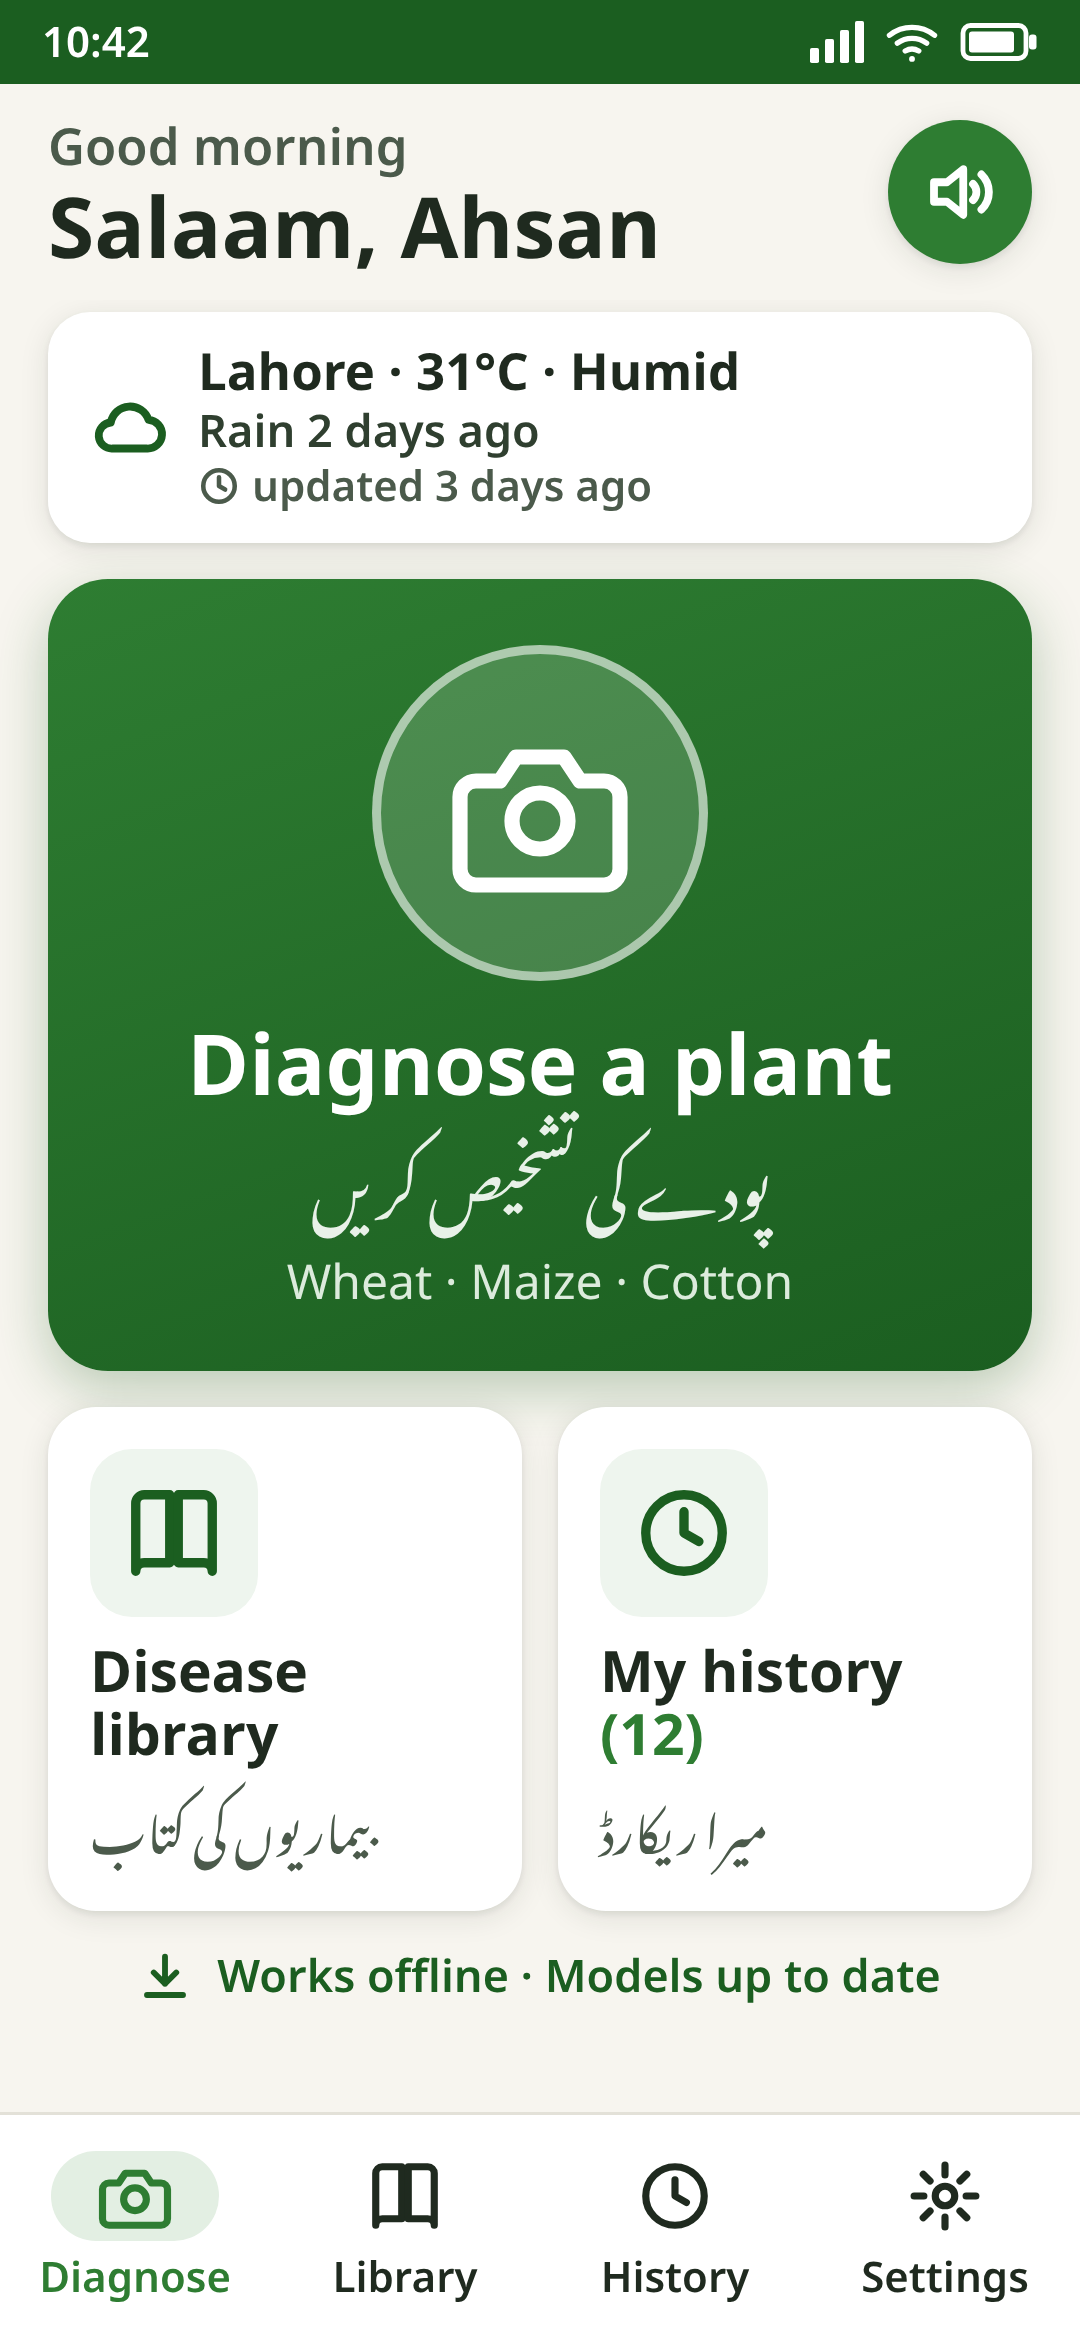
\includegraphics[width=0.3\textwidth]{Figures/gui/03_home.png}
  \caption{Left: language selection with spoken language names (UC-01). Centre: sign-in with a WhatsApp code and the ``Skip for now'' option (UC-02, UC-03). Right: Home with the Diagnose card, the weather chip showing the district and the age of the data (UC-13), and the library and history entries.}
  \label{fig:gui1}
\end{figure}

\begin{figure}[H]
  \centering
  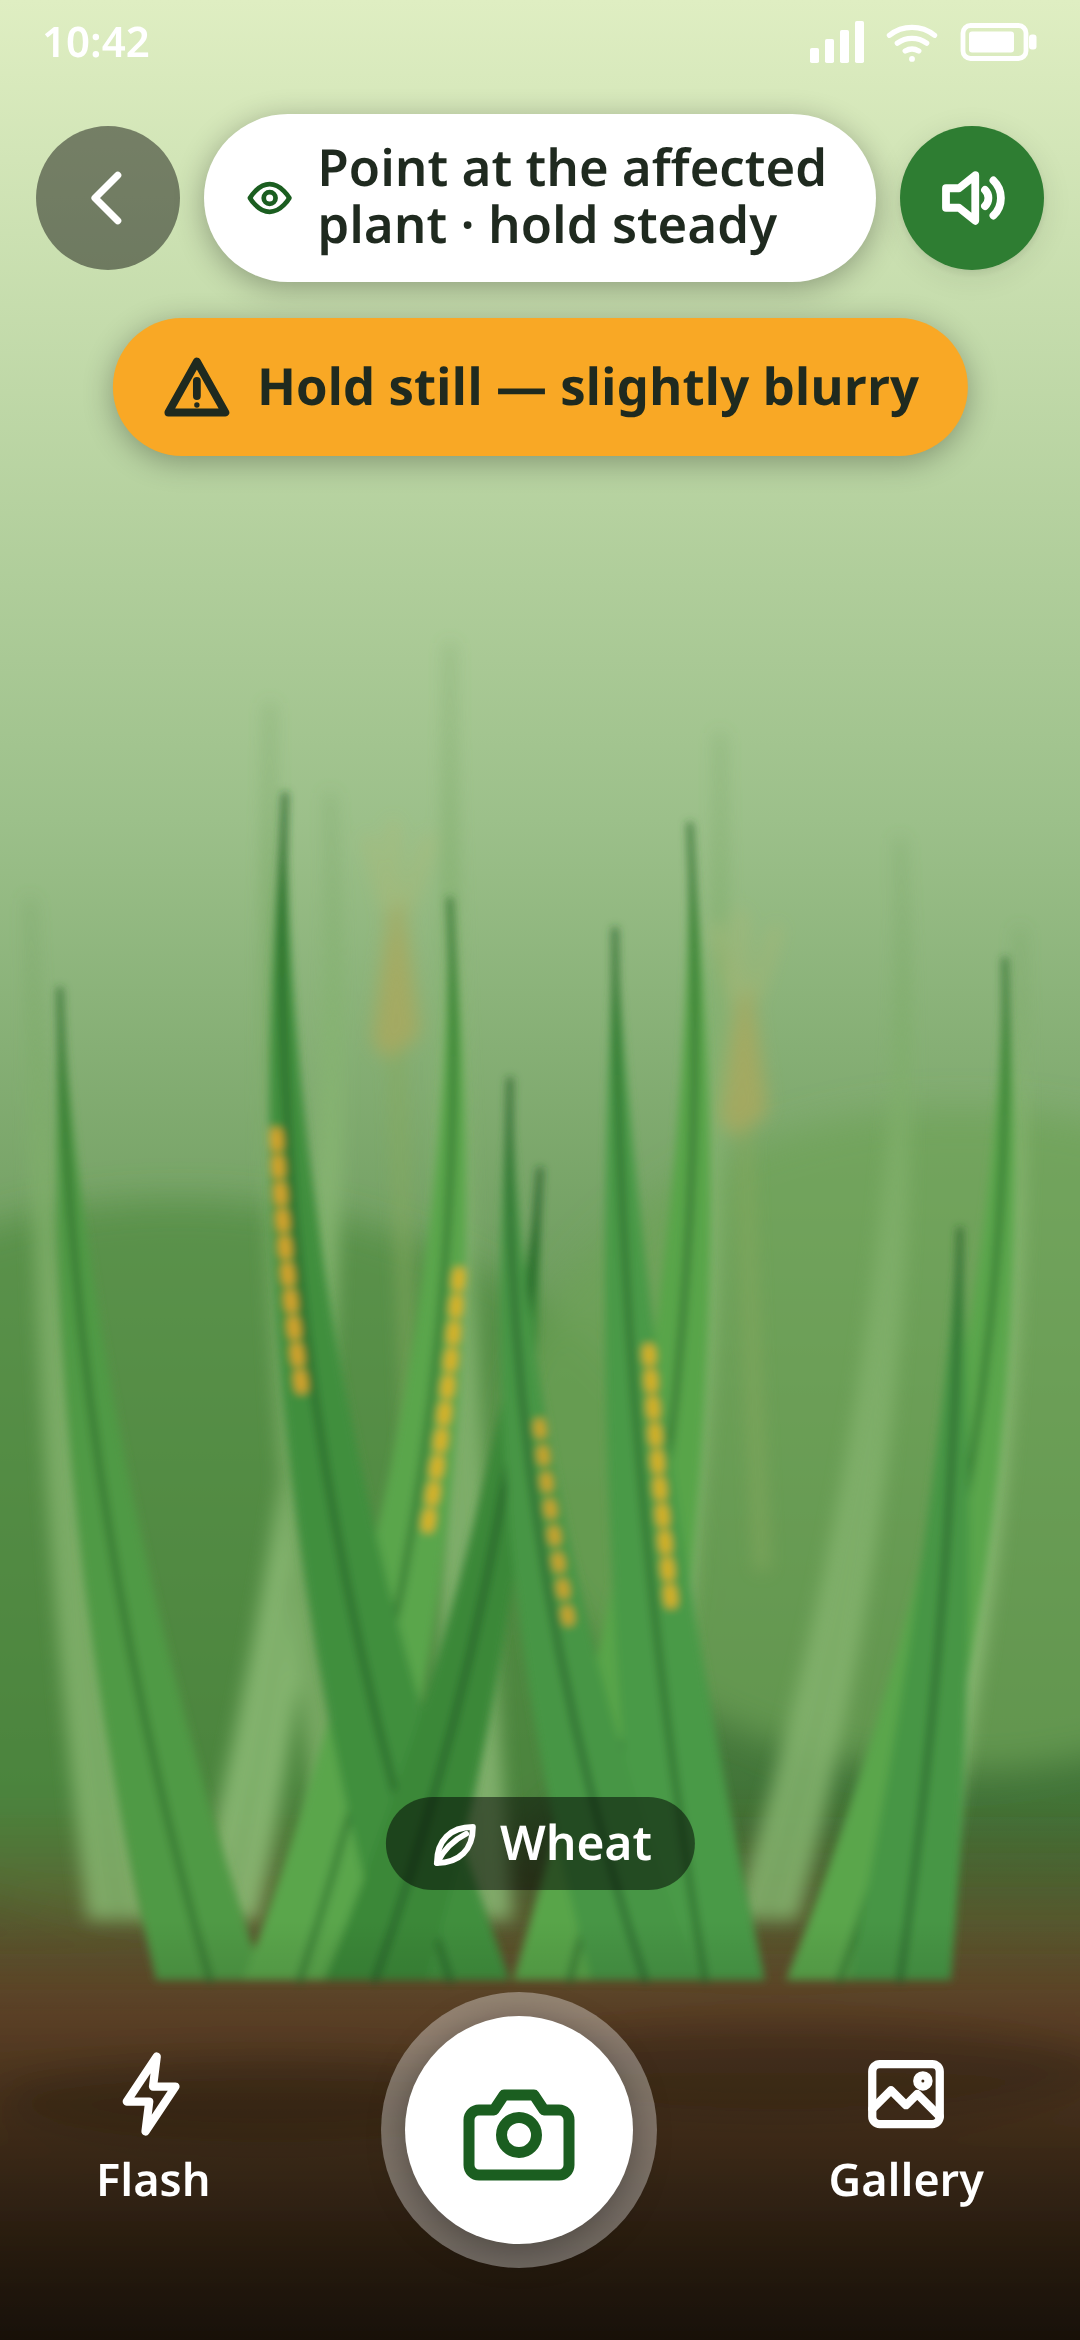
\includegraphics[width=0.3\textwidth]{Figures/gui/04_camera.png}\hspace{0.03\textwidth}
  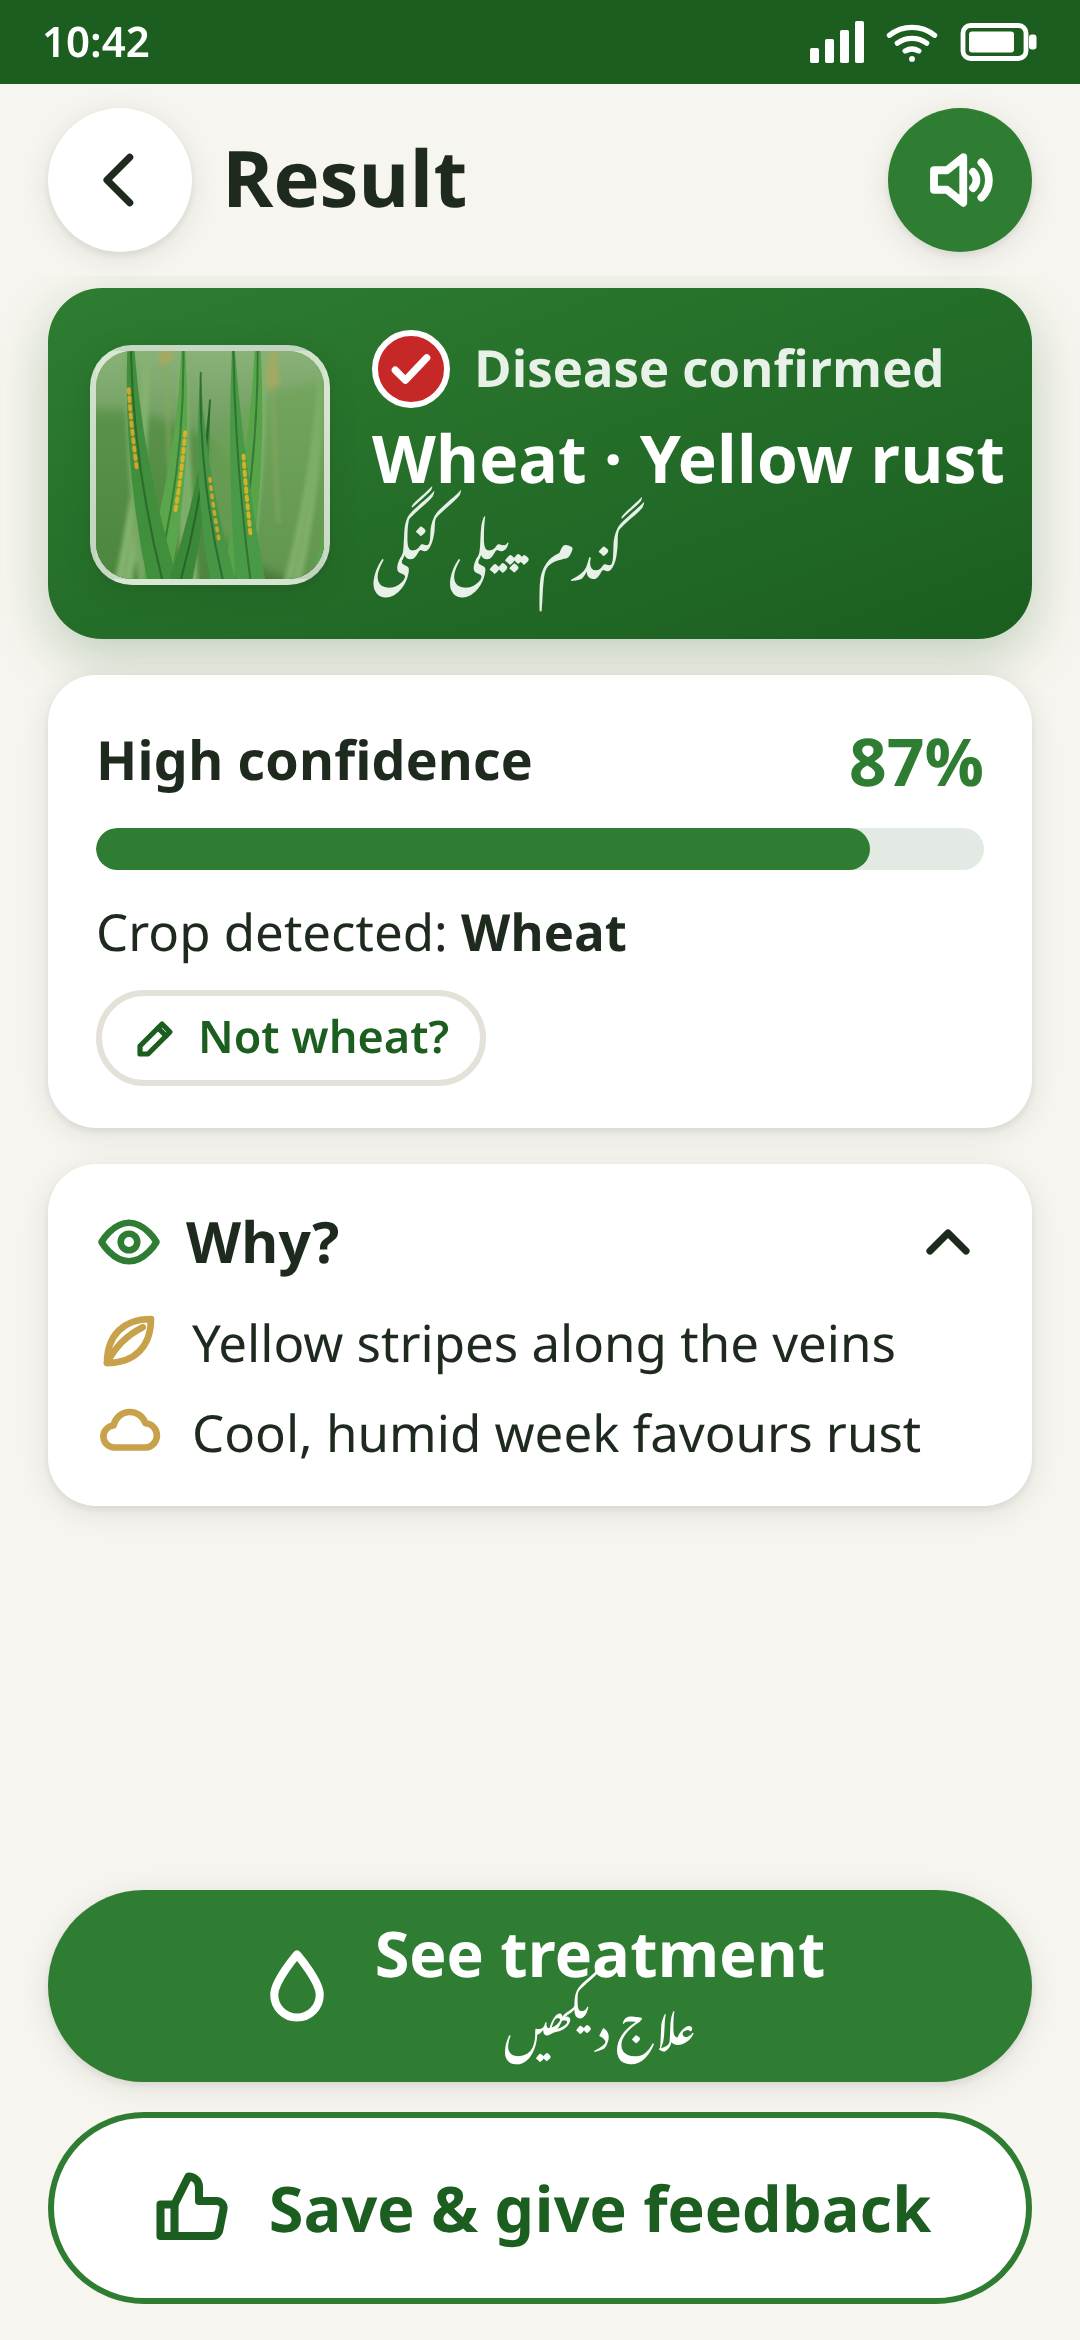
\includegraphics[width=0.3\textwidth]{Figures/gui/05_result_confident.png}\hspace{0.03\textwidth}
  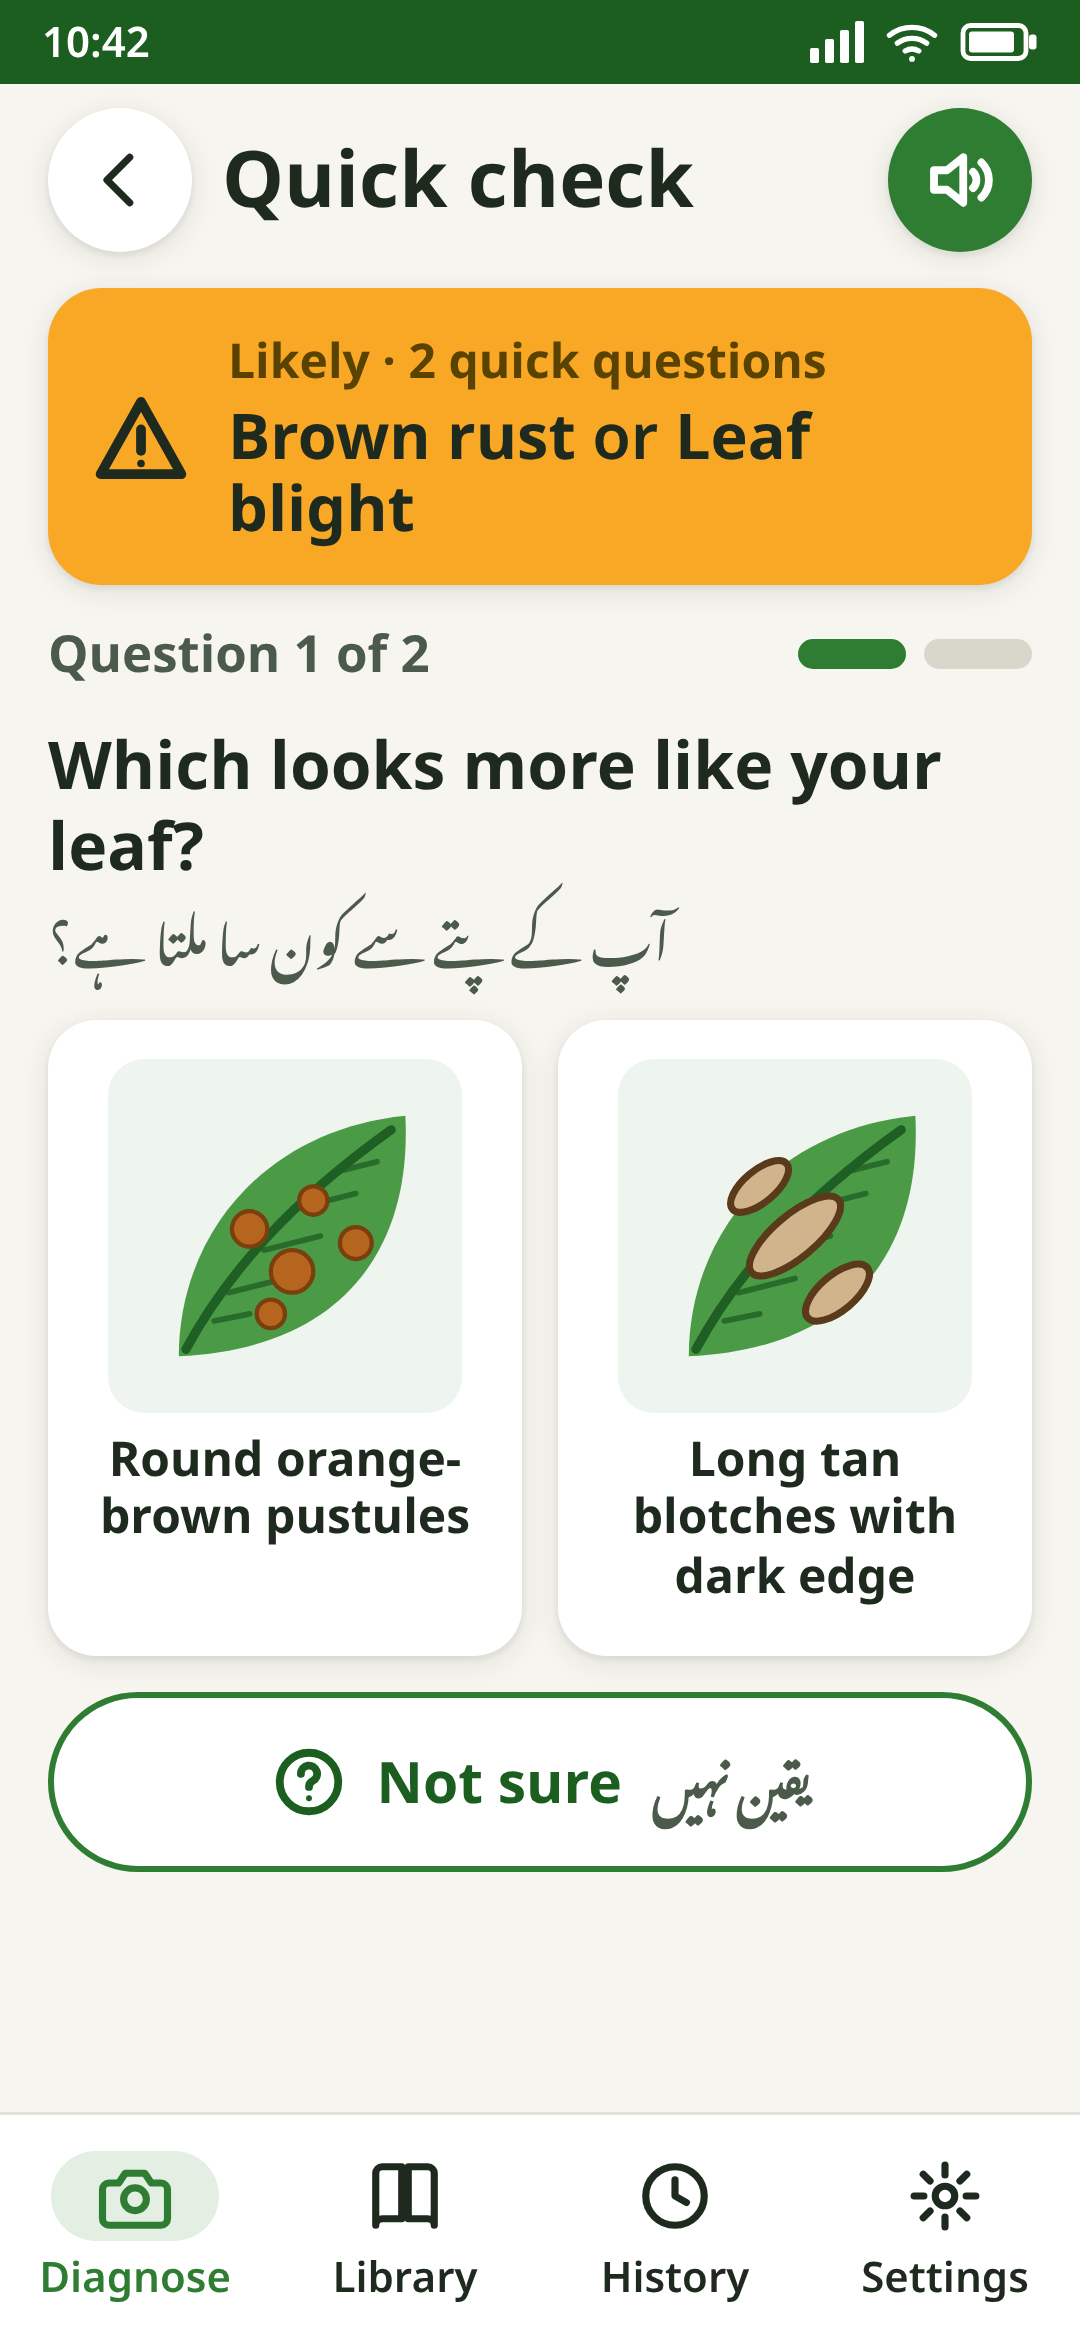
\includegraphics[width=0.3\textwidth]{Figures/gui/06_result_followup.png}
  \caption{Left: camera pointed at the affected plant, with the live blur warning (UC-04). Centre: Confident result with badge, confidence bar, detected-crop chip with correction (UC-05, UC-06) and the Why panel. Right: Likely result asking a picture-based follow-up question (UC-07).}
  \label{fig:gui2}
\end{figure}

\begin{figure}[H]
  \centering
  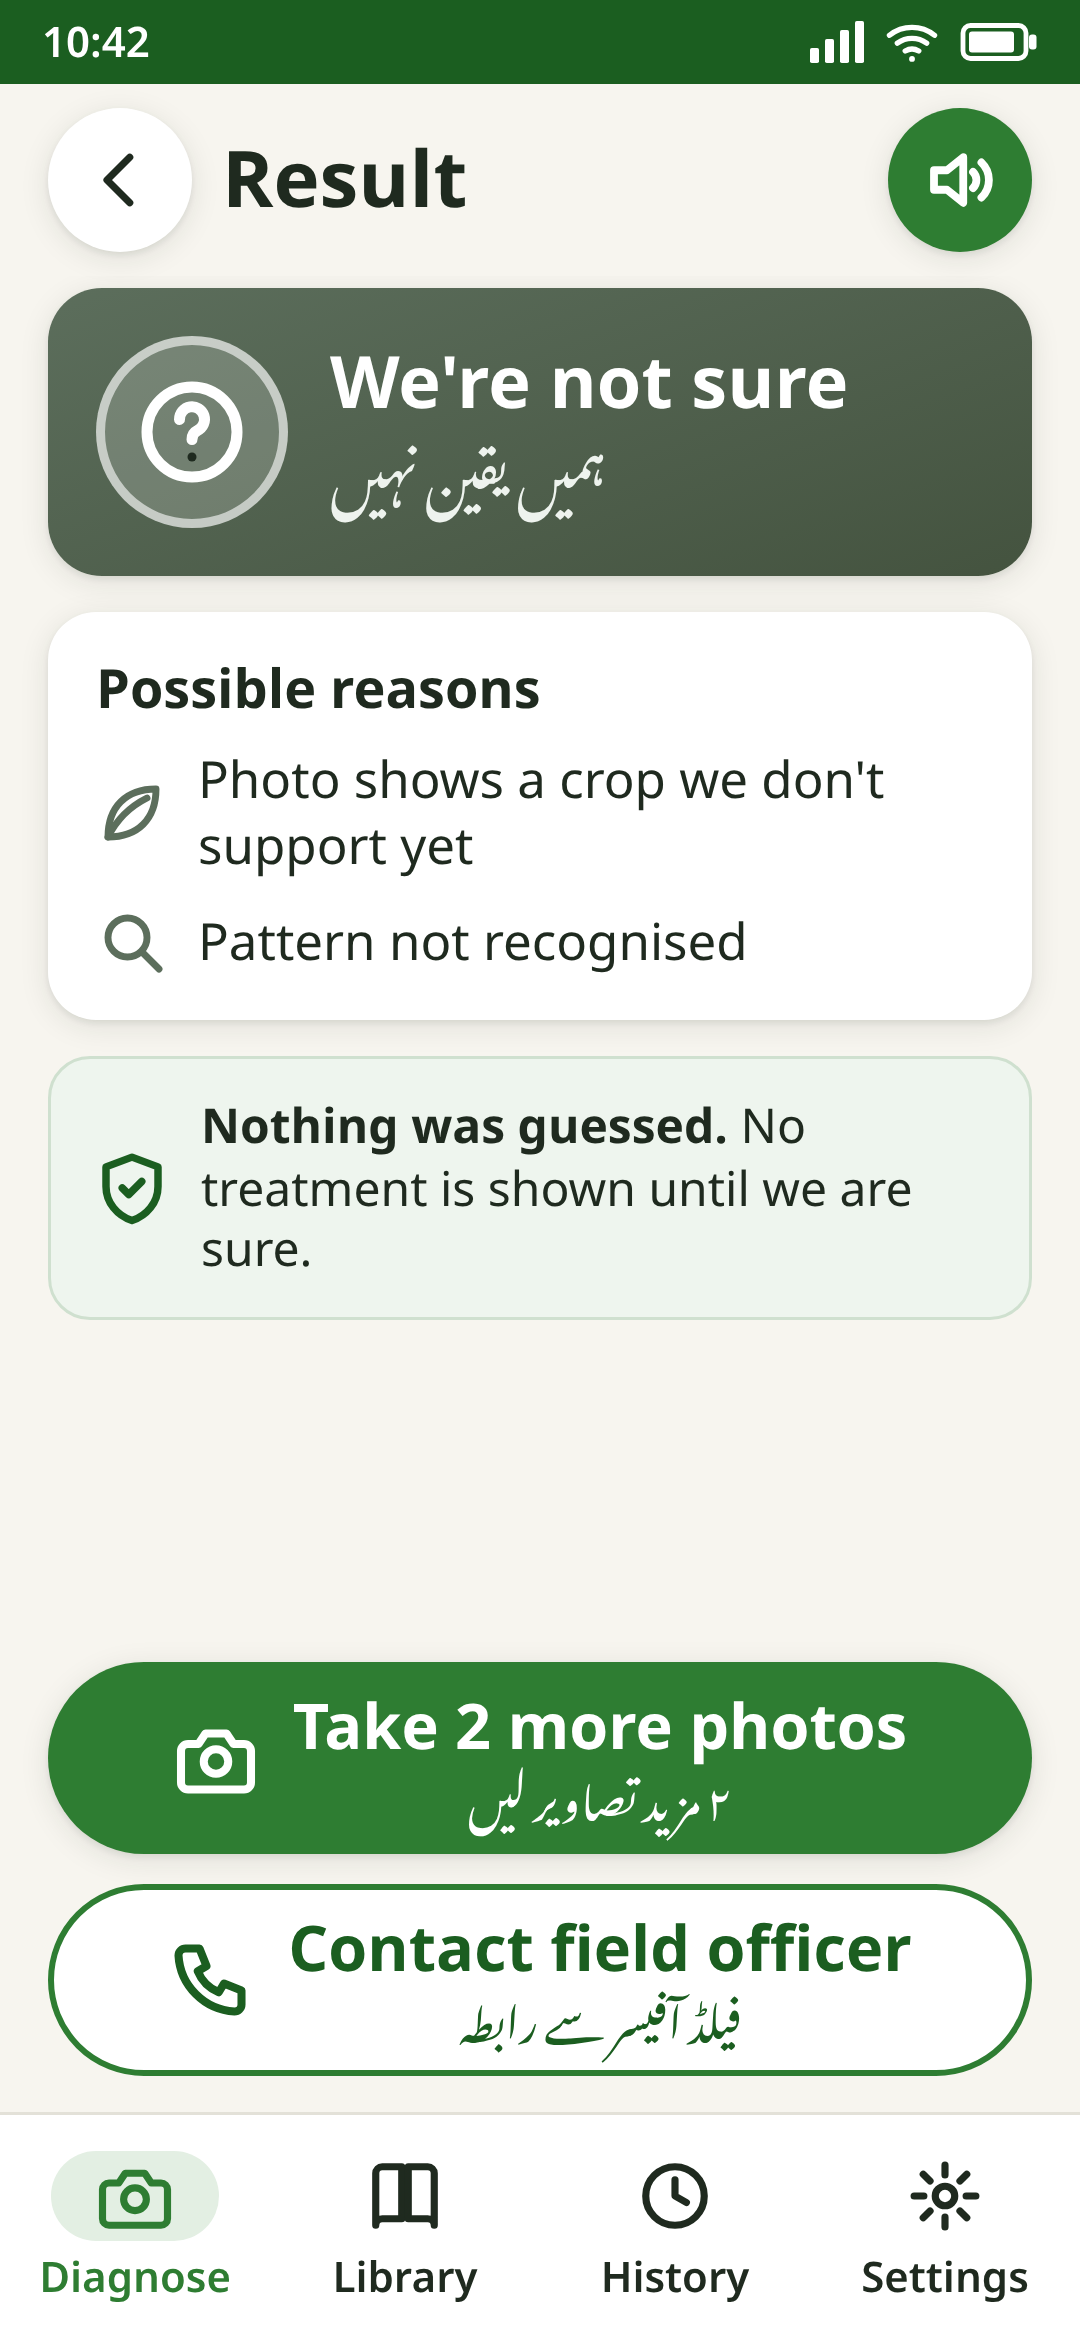
\includegraphics[width=0.3\textwidth]{Figures/gui/07_result_unsure.png}\hspace{0.03\textwidth}
  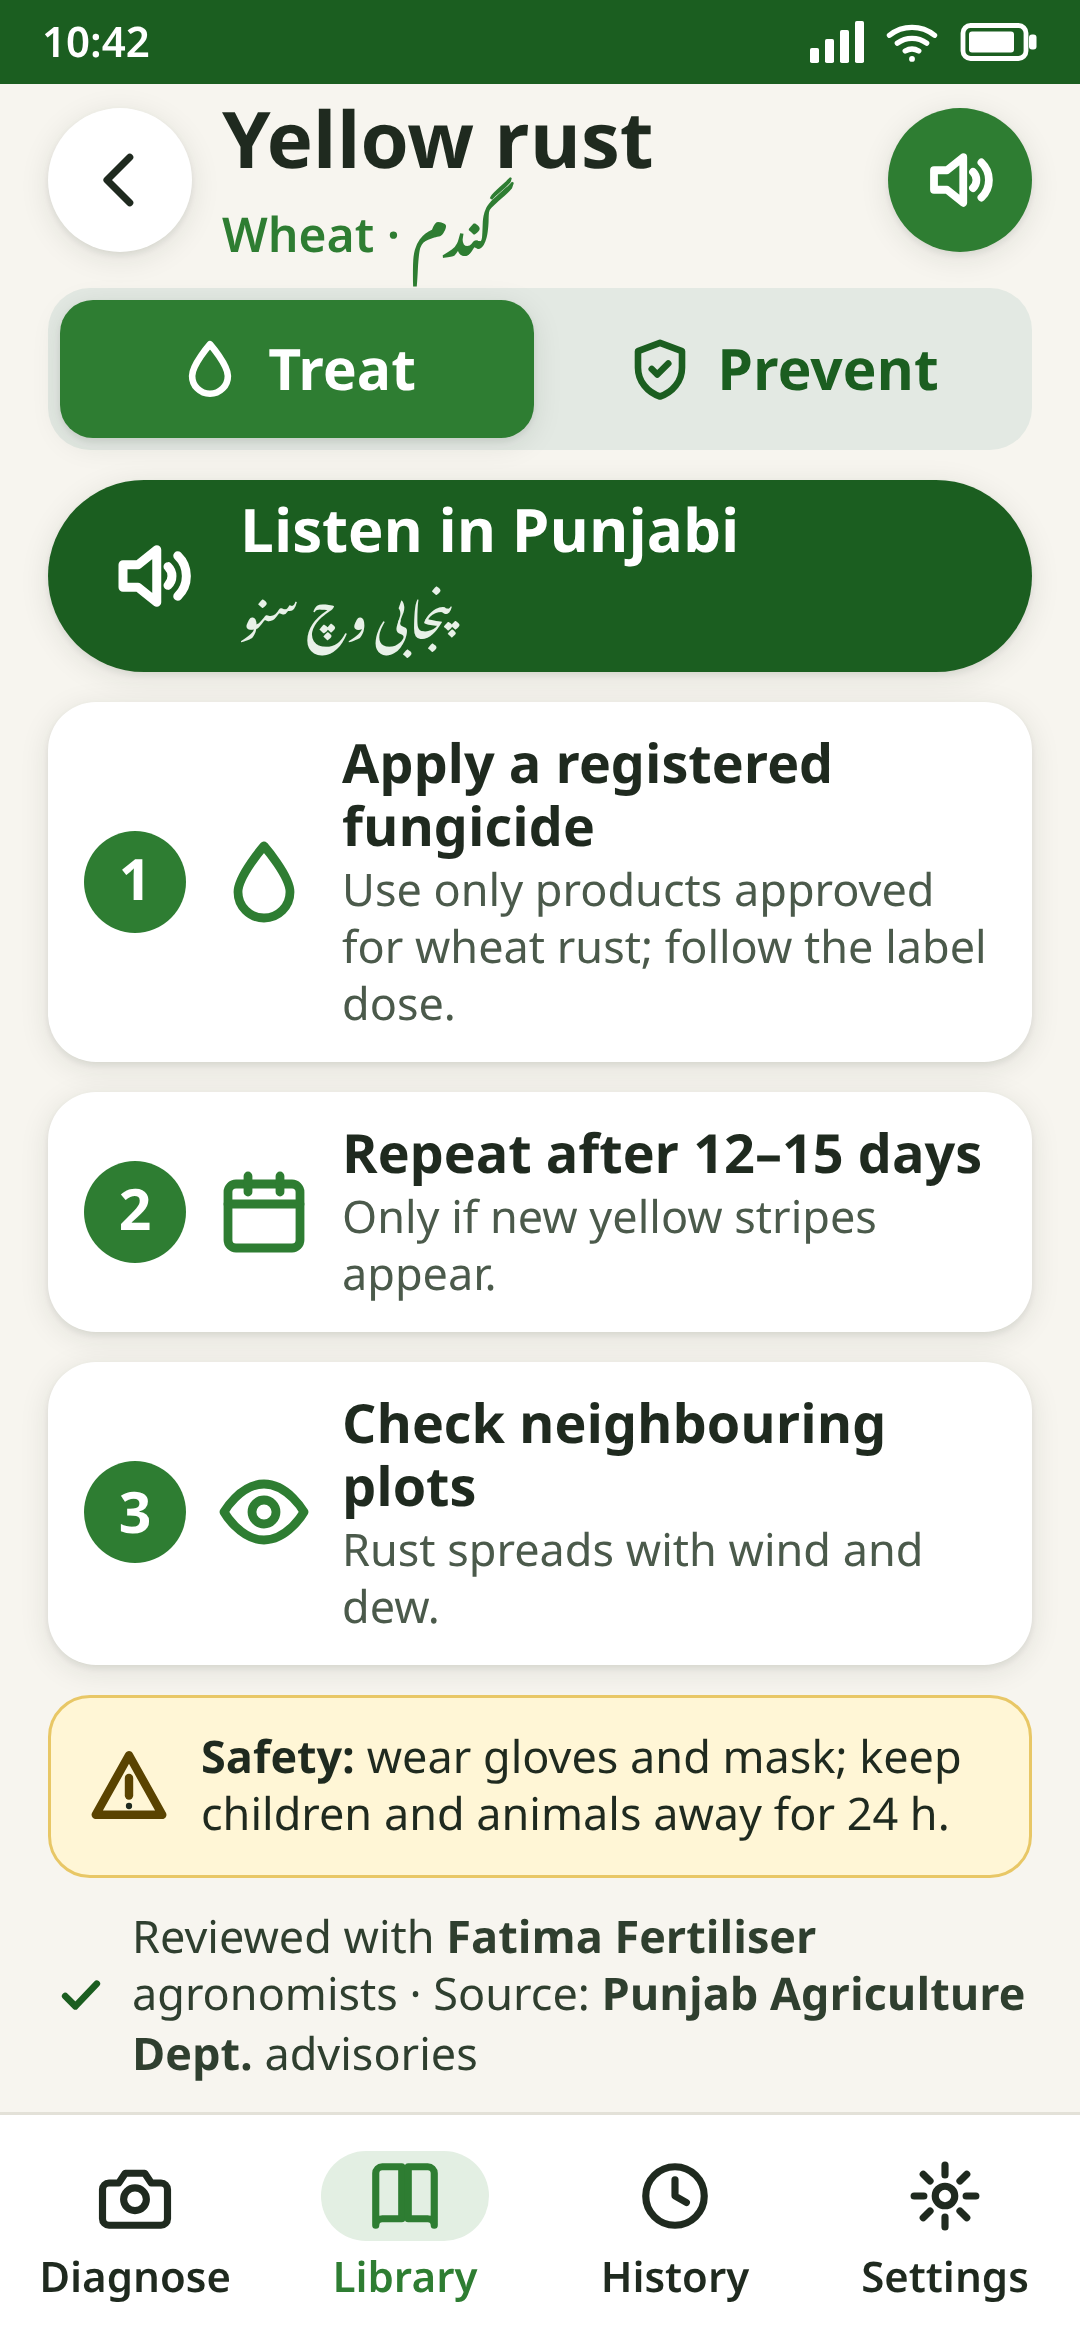
\includegraphics[width=0.3\textwidth]{Figures/gui/08_remedy.png}\hspace{0.03\textwidth}
  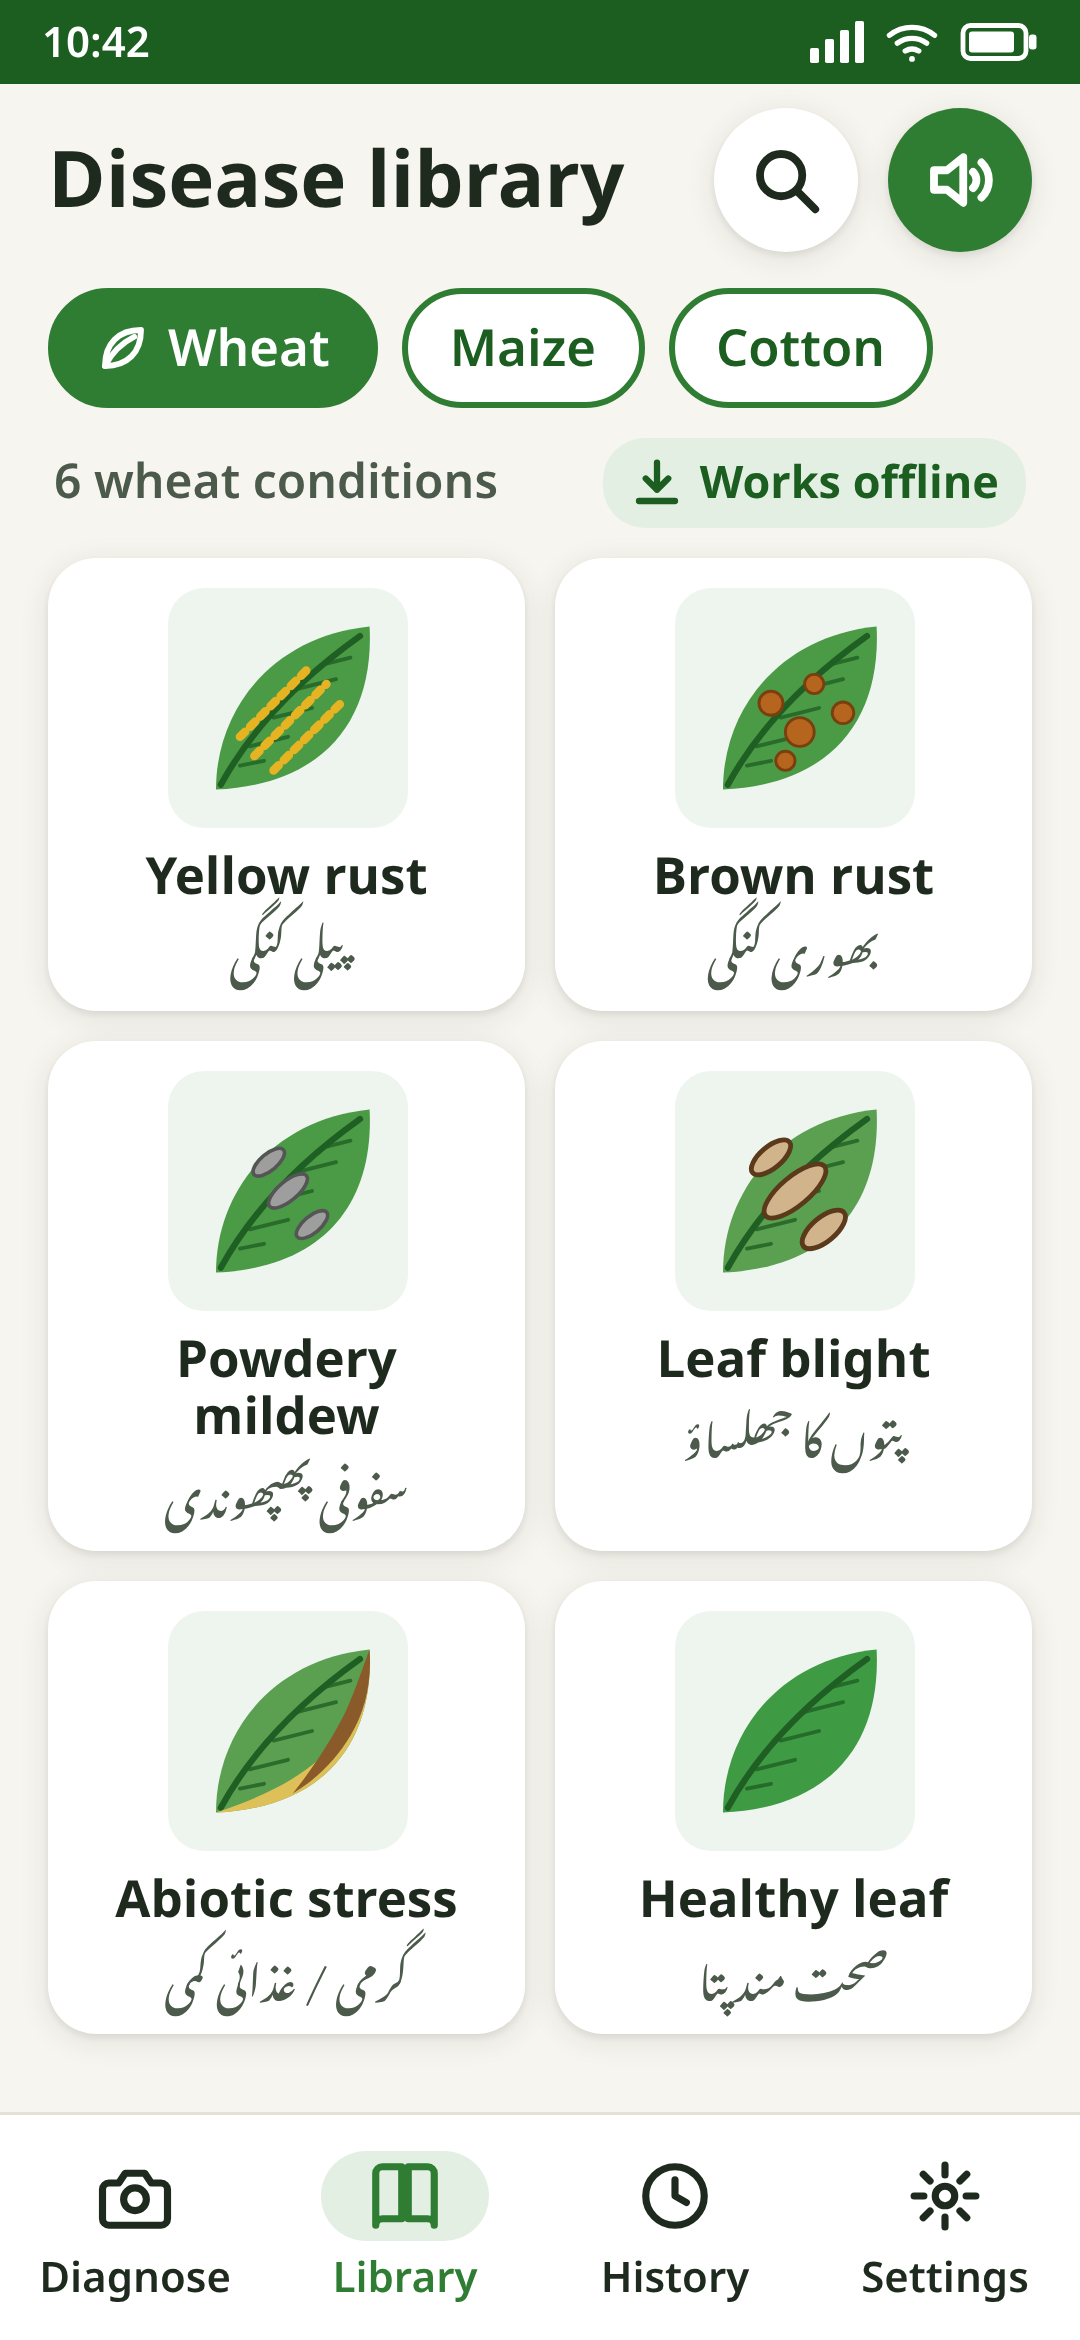
\includegraphics[width=0.3\textwidth]{Figures/gui/09_library.png}
  \caption{Left: Unsure result with reasons and the two actions (UC-08). Centre: treatment screen with Treat and Prevent tabs, numbered steps, safety note, audio button and attribution (UC-09). Right: offline disease library filtered to wheat (UC-10).}
  \label{fig:gui3}
\end{figure}

\begin{figure}[H]
  \centering
  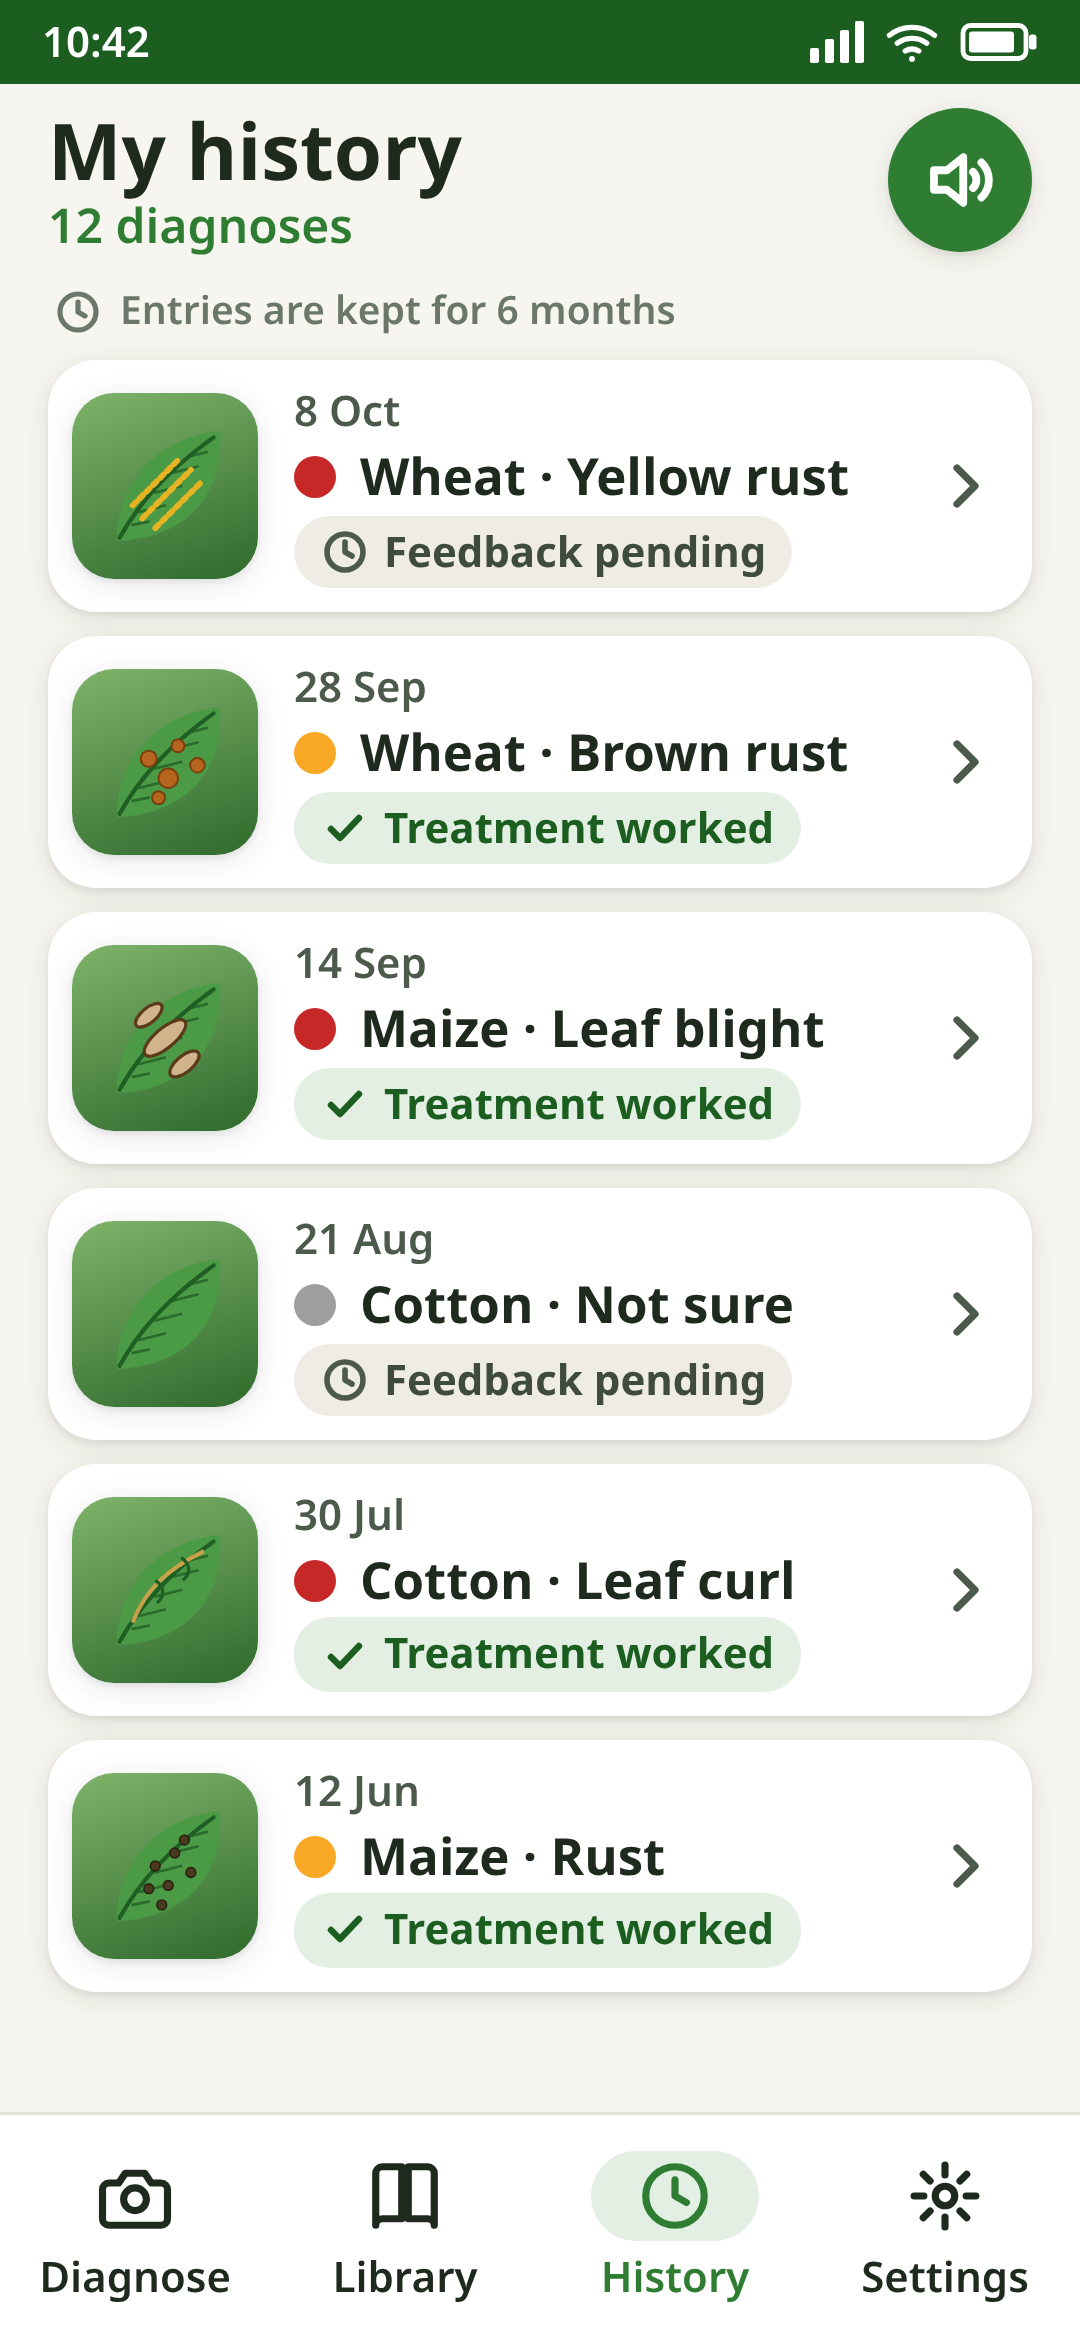
\includegraphics[width=0.3\textwidth]{Figures/gui/10_history.png}\hspace{0.03\textwidth}
  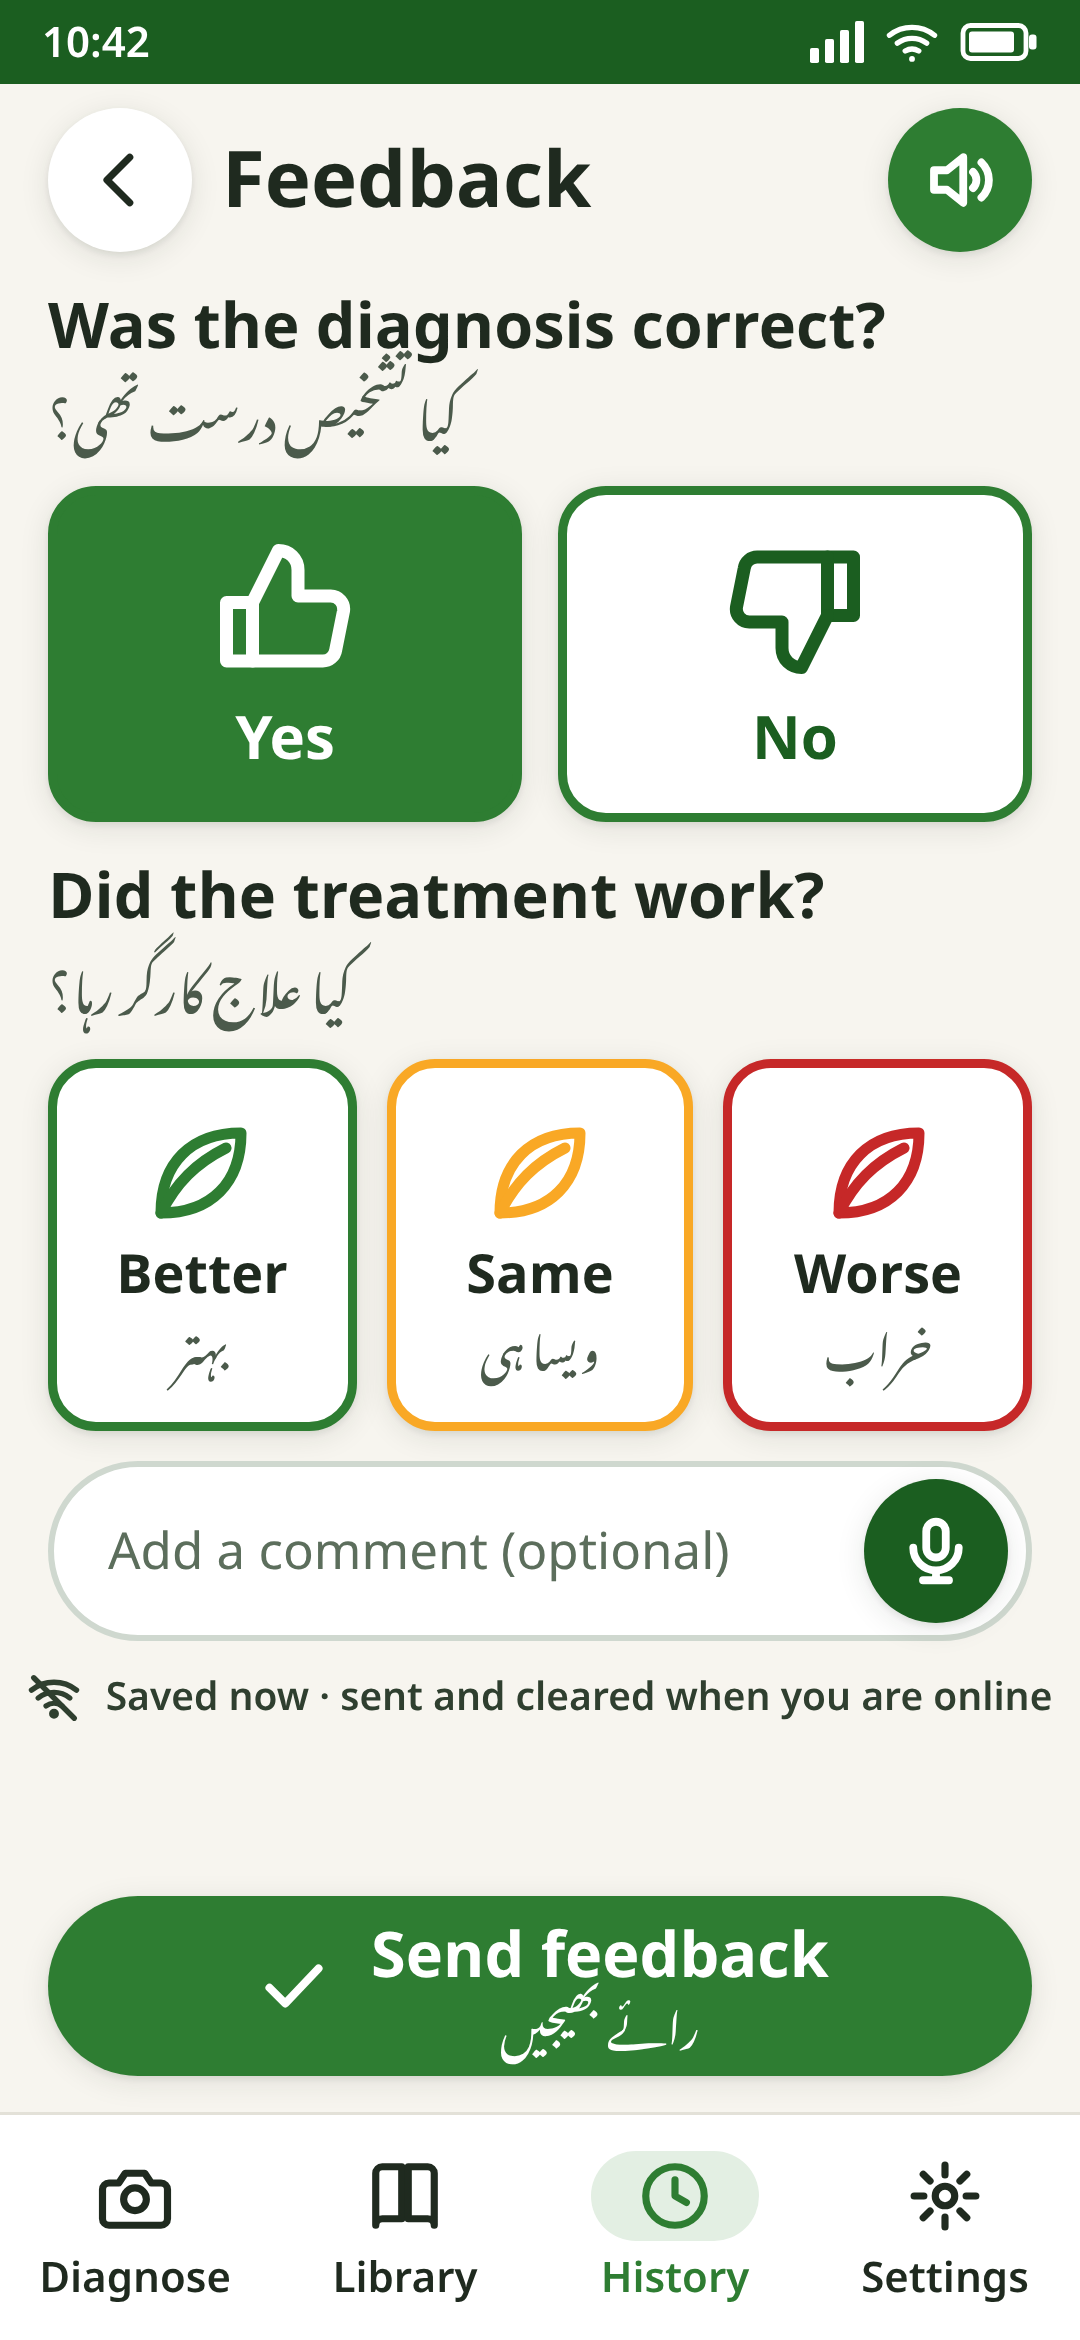
\includegraphics[width=0.3\textwidth]{Figures/gui/11_feedback.png}
  \caption{Left: history of recent diagnoses with outcome colours and feedback status (UC-11). Right: feedback screen with large icon options and the ``saved now, sent when online'' note (UC-12).}
  \label{fig:gui4}
\end{figure}

\section{Database Design}
\label{sec:db}
KhetLens has two data stores. On the phone, a Room (SQLite) database holds the farmer's profile, the last six months of diagnoses, weather snapshots and feedback awaiting upload, together with a read-only copy of the content pack for fast lookup. On the server, PostgreSQL holds users, feedback records, shared images (only when the farmer opts in), content and model versions, and the district list. Both are relational because the data are small, well structured and need transactional integrity.

\subsection{ER Diagram}
Figure~\ref{fig:er} shows the two stores. The phone holds everything the farmer needs; the server holds only what is needed for verification, feedback aggregation and distribution.

\begin{figure}[H]
  \centering
  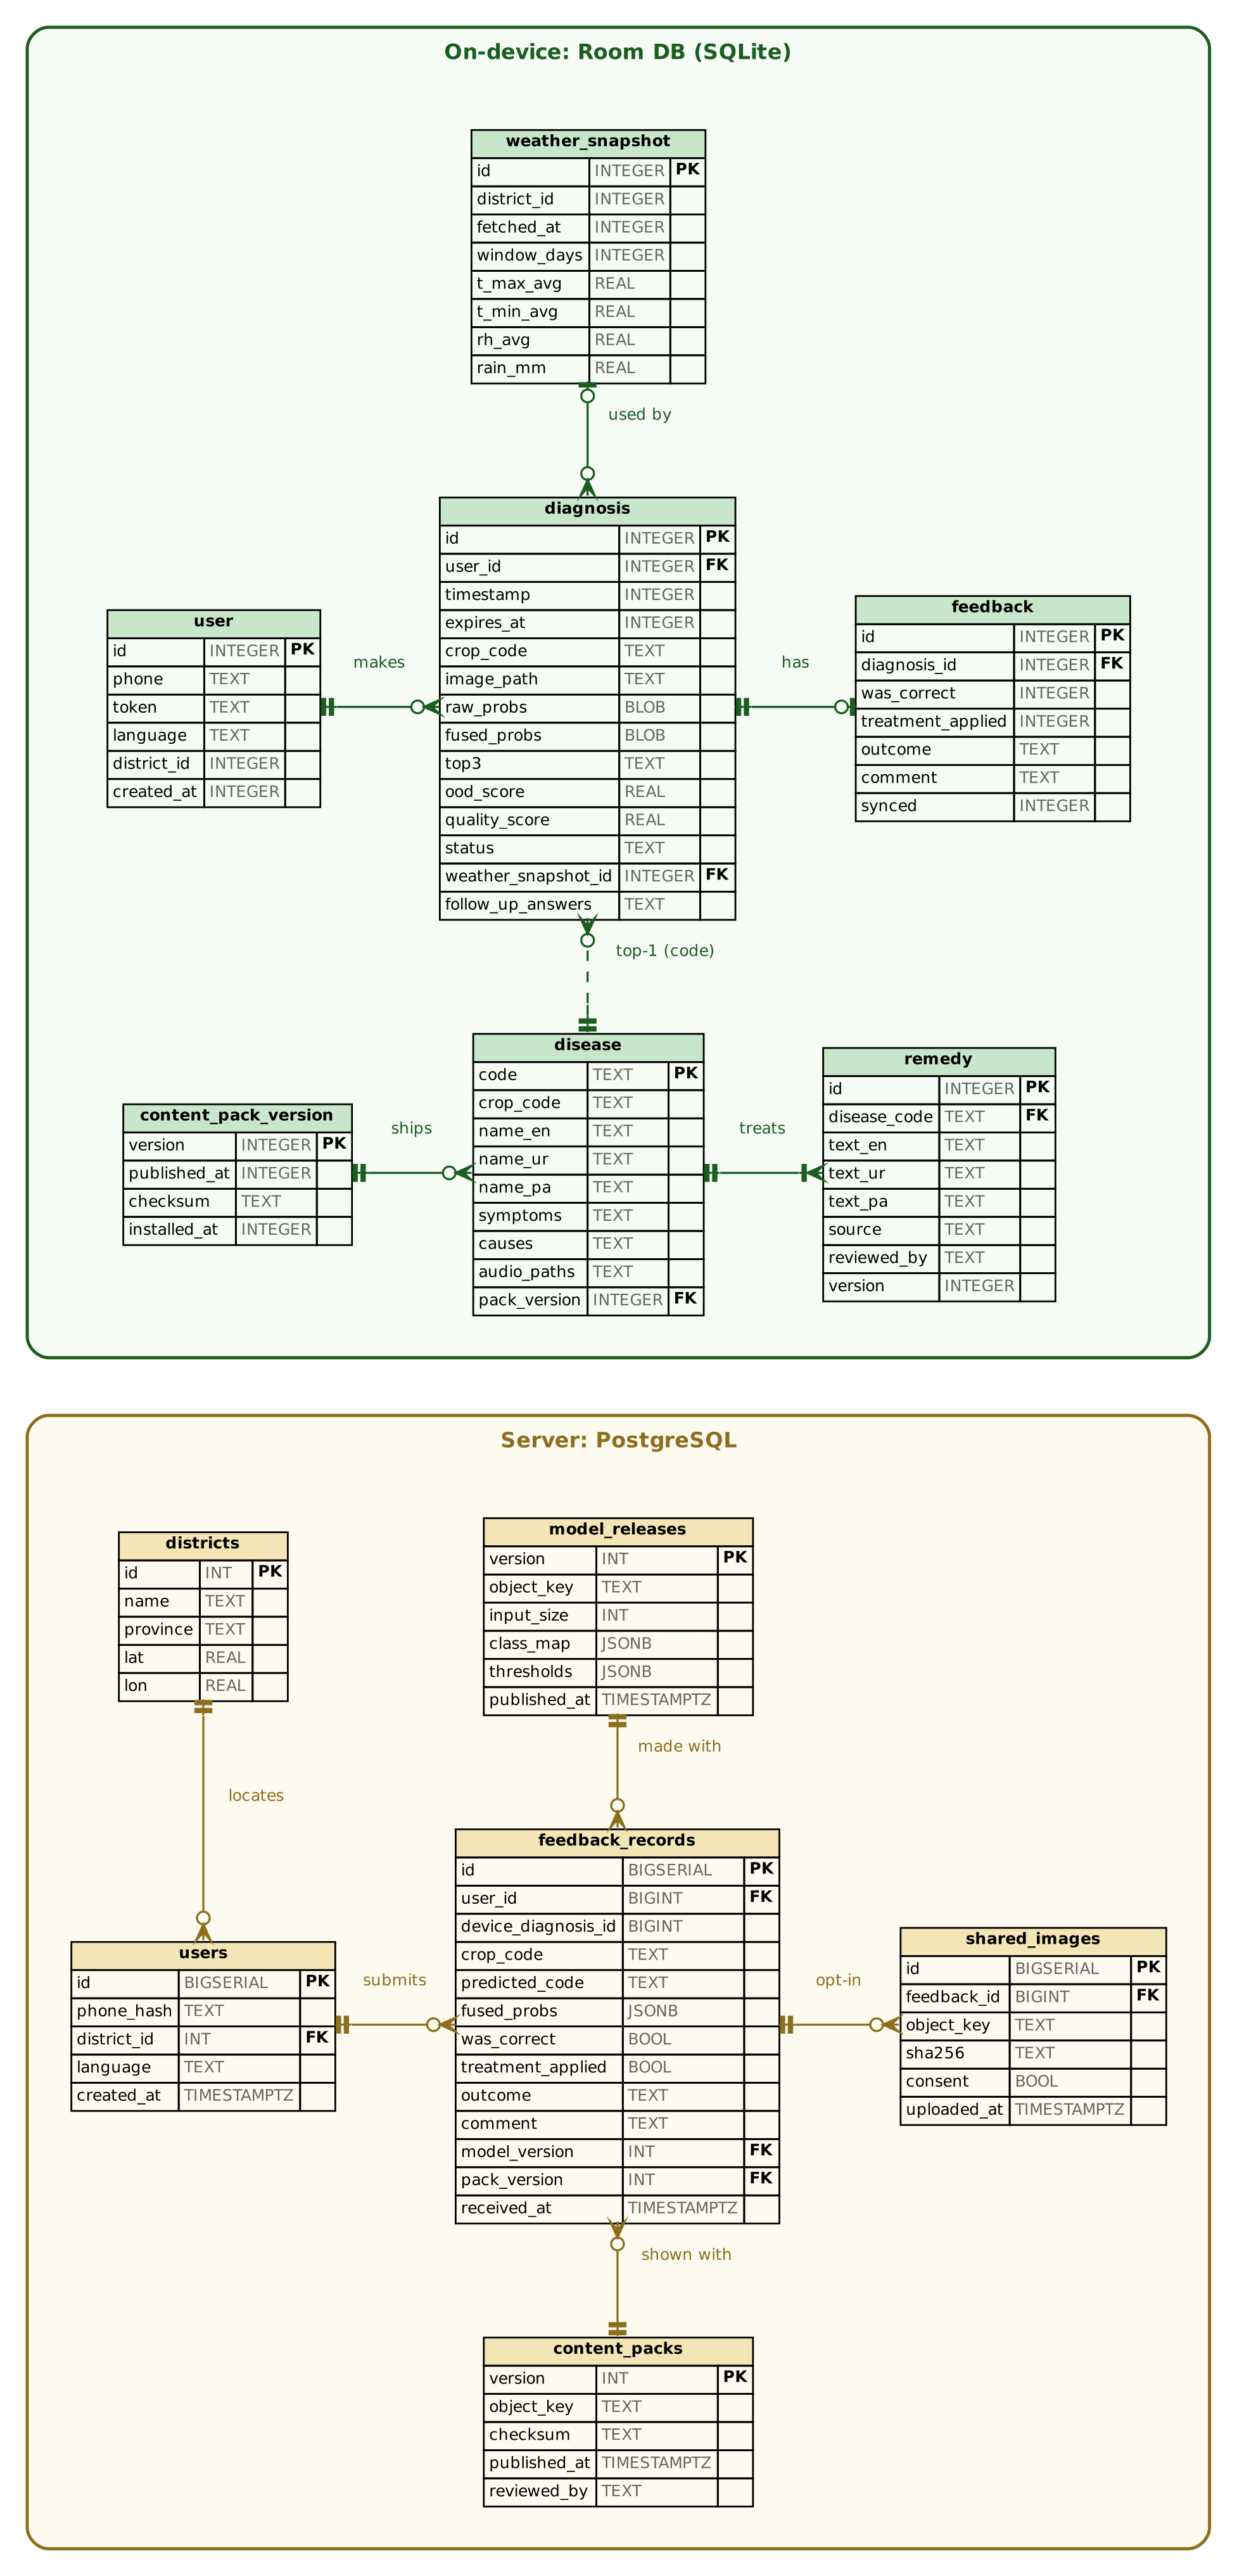
\includegraphics[width=\textwidth,height=0.88\textheight,keepaspectratio]{Figures/diagrams/er_diagram.png}
  \caption{Entity-relationship diagram of the on-device database (top) and the server database (bottom).}
  \label{fig:er}
\end{figure}

\subsection{Data Dictionary}
Tables~\ref{tab:dd-device} and~\ref{tab:dd-server} list every table of the two stores, one attribute per row. PK marks a primary key and FK a foreign key.

\newcommand{\ddtable}[1]{\multicolumn{3}{|l|}{\cellcolor{gray!12}\textbf{Table: #1}} \\ \hline}
{\small
\begin{longtable}{|L{4.0cm}|L{2.6cm}|L{8.0cm}|}
\caption{Data dictionary: on-device database.}\label{tab:dd-device}\\
\hline
\textbf{Attribute} & \textbf{Type} & \textbf{Description} \\ \hline
\endfirsthead
\multicolumn{3}{l}{\small\textit{Table \thetable\ continued}}\\ \hline
\textbf{Attribute} & \textbf{Type} & \textbf{Description} \\ \hline
\endhead
\hline \multicolumn{3}{r}{\small\textit{continued on next page}}\\
\endfoot
\endlastfoot
\ddtable{user}
id (PK) & TEXT & Local profile identifier. \\ \hline
phone & TEXT, null & Mobile number; null for guests. \\ \hline
token & TEXT, null & Reference to the sign-in token in encrypted storage. \\ \hline
language & TEXT & en, ur or pa. \\ \hline
district\_id (FK) & INTEGER & Farmer's district. \\ \hline
created\_at & INTEGER & Profile creation time. \\ \hline
\ddtable{diagnosis}
id (PK) & TEXT & Diagnosis identifier. \\ \hline
user\_id (FK) & TEXT & Owner. \\ \hline
timestamp & INTEGER & Capture time. \\ \hline
expires\_at & INTEGER & Automatic deletion time (six months after capture). \\ \hline
crop\_code & TEXT & WHT, MZE or COT. \\ \hline
crop\_corrected & INTEGER & 1 if the farmer changed the detected crop. \\ \hline
image\_path & TEXT & App-private path of the photograph. \\ \hline
raw\_probs & JSON & Class probabilities before the weather prior. \\ \hline
fused\_probs & JSON & Class probabilities after the weather prior. \\ \hline
top1\_code (FK) & TEXT, null & Final condition; null for Unsure. \\ \hline
confidence & REAL & Calibrated confidence of the final condition. \\ \hline
ood\_score & REAL & Novelty score (feature distance). \\ \hline
quality\_score & REAL & Image quality score. \\ \hline
status & TEXT & CONFIDENT, LIKELY or UNSURE. \\ \hline
weather\_snapshot\_id (FK) & TEXT, null & Snapshot used, if any. \\ \hline
followup\_answers & JSON & Question and option identifiers. \\ \hline
model\_version & TEXT & Model release used. \\ \hline
\ddtable{weather\_snapshot}
id (PK) & TEXT & Snapshot identifier. \\ \hline
district\_id & INTEGER & District. \\ \hline
fetched\_at & INTEGER & Fetch time. \\ \hline
tmax\_avg & REAL & Mean daily maximum temperature over 14 days. \\ \hline
tmin\_avg & REAL & Mean daily minimum temperature over 14 days. \\ \hline
rh\_avg & REAL & Mean relative humidity over 14 days. \\ \hline
rain\_mm & REAL & Total rainfall over 14 days. \\ \hline
days\_since\_rain & INTEGER & Days since the last rain. \\ \hline
\ddtable{feedback (row deleted once the server acknowledges it)}
id (PK) & TEXT & Feedback identifier. \\ \hline
diagnosis\_id (FK) & TEXT & One feedback per diagnosis. \\ \hline
was\_correct & INTEGER, null & 1 yes, 0 no. \\ \hline
stated\_condition & TEXT, null & Farmer's own answer if ``no''. \\ \hline
outcome & TEXT, null & BETTER, SAME or WORSE. \\ \hline
comment & TEXT, null & Optional comment. \\ \hline
share\_image & INTEGER & 1 if the farmer opted in to share the photograph. \\ \hline
synced & INTEGER & 0 while awaiting upload. \\ \hline
\ddtable{condition}
code (PK) & TEXT & e.g.\ WHT\_YRUST. \\ \hline
crop\_code & TEXT & Crop. \\ \hline
name\_en, name\_ur, name\_pa & TEXT & Names in the three languages. \\ \hline
symptoms, causes & JSON & Per-language text. \\ \hline
audio\_paths & JSON & Per-language audio files. \\ \hline
\ddtable{remedy}
id (PK) & TEXT & Guidance identifier. \\ \hline
condition\_code (FK) & TEXT & Condition. \\ \hline
kind & TEXT & TREAT or PREVENT. \\ \hline
steps & JSON & Ordered per-language steps. \\ \hline
safety\_note & JSON & Per-language safety note. \\ \hline
source, reviewed\_by, reviewed\_on & TEXT & Attribution (mandatory). \\ \hline
\ddtable{content\_pack\_version}
version (PK) & TEXT & Installed content version. \\ \hline
checksum & TEXT & Checksum of the installed pack. \\ \hline
installed\_at & INTEGER & Install time. \\ \hline
\end{longtable}
}

{\small
\begin{longtable}{|L{4.0cm}|L{2.6cm}|L{8.0cm}|}
\caption{Data dictionary: server database.}\label{tab:dd-server}\\
\hline
\textbf{Attribute} & \textbf{Type} & \textbf{Description} \\ \hline
\endfirsthead
\multicolumn{3}{l}{\small\textit{Table \thetable\ continued}}\\ \hline
\textbf{Attribute} & \textbf{Type} & \textbf{Description} \\ \hline
\endhead
\hline \multicolumn{3}{r}{\small\textit{continued on next page}}\\
\endfoot
\endlastfoot
\ddtable{users}
id (PK) & UUID & Server user identifier. \\ \hline
phone\_hash & TEXT & Salted hash of the number; the number itself is not kept. \\ \hline
district\_id (FK) & INTEGER & District. \\ \hline
language & TEXT & Preferred language. \\ \hline
created\_at, last\_seen & TIMESTAMP & Audit fields. \\ \hline
\ddtable{feedback\_records}
id (PK) & UUID & Mirrors the device feedback id. \\ \hline
user\_id (FK) & UUID & Submitter. \\ \hline
district\_id (FK) & INTEGER & District at diagnosis. \\ \hline
crop\_code, predicted\_code & TEXT & Crop and condition predicted by the model. \\ \hline
status, confidence & TEXT, REAL & Outcome and calibrated confidence. \\ \hline
was\_correct & SMALLINT & Farmer's answer. \\ \hline
stated\_condition & TEXT & Farmer's own answer if ``no''. \\ \hline
outcome, comment & TEXT & Treatment outcome and comment. \\ \hline
model\_version, pack\_version (FK) & TEXT & Versions in use. \\ \hline
diagnosed\_at, received\_at & TIMESTAMP & Timestamps. \\ \hline
\ddtable{shared\_images (only when the farmer opted in)}
id (PK) & UUID & Image identifier. \\ \hline
feedback\_id (FK) & UUID & Linked feedback. \\ \hline
object\_key & TEXT & Storage key. \\ \hline
label\_status & TEXT & UNLABELLED, LABELLED or REJECTED. \\ \hline
\ddtable{content\_packs}
version (PK) & TEXT & Semantic version. \\ \hline
object\_key, checksum & TEXT & File location and checksum. \\ \hline
published\_at & TIMESTAMP & Release time. \\ \hline
reviewed\_by & TEXT & Reviewing agronomist. \\ \hline
\ddtable{model\_releases}
version (PK) & TEXT & Semantic version. \\ \hline
object\_key, checksum & TEXT & File location and checksum. \\ \hline
input\_size & INTEGER & Model input size in pixels. \\ \hline
class\_map & JSON & Class indices to condition codes. \\ \hline
thresholds & JSON & Thresholds used by the uncertainty check. \\ \hline
field\_macro\_f1 & REAL & Acceptance metric for the release. \\ \hline
published\_at & TIMESTAMP & Release time. \\ \hline
\ddtable{districts}
id (PK) & INTEGER & District identifier. \\ \hline
name\_en, name\_ur & TEXT & Names. \\ \hline
centroid\_lat, centroid\_lon & REAL & Centroid for weather queries. \\ \hline
\end{longtable}
}

\section{Risk Analysis}
\label{sec:risks}
{\small
\begin{longtable}{|L{0.9cm}|L{4.2cm}|L{0.5cm}|L{0.5cm}|L{7.7cm}|}
\caption{Risk register. L = likelihood, I = impact, each rated High (H), Medium (M) or Low (L).}\label{tab:risks}\\
\hline
\textbf{ID} & \textbf{Risk} & \textbf{L} & \textbf{I} & \textbf{Mitigation} \\ \hline
\endfirsthead
\multicolumn{5}{l}{\small\textit{Table \thetable\ continued}}\\ \hline
\textbf{ID} & \textbf{Risk} & \textbf{L} & \textbf{I} & \textbf{Mitigation} \\ \hline
\endhead
\hline \multicolumn{5}{r}{\small\textit{continued on next page}}\\
\endfoot
\endlastfoot
R-01 & Local field photographs arrive later or in smaller numbers than planned. & M & H & Start from public field datasets from several regions; collect photographs on university and nearby farms; design the field-data study so that any number of local images still gives a useful curve. \\ \hline
R-02 & Accuracy on field photographs below target. & M & H & Mixed-source training, background augmentation, distillation, and domain adaptation with unlabelled field images; report results honestly against the target. \\ \hline
R-03 & 8-bit quantisation reduces accuracy or does not speed up inference. & M & M & Quantisation-aware training with a field calibration set; compare runtimes on the target phones; fall back to 16-bit floats if needed. \\ \hline
R-04 & Inference slower than intended on entry-level phones. & M & M & Benchmark early; reduce input size; switch to MobileNetV3-Small; keep the model loaded between diagnoses. \\ \hline
R-05 & Weather prior harms accuracy on some classes. & M & M & Per-class ablation on the field test set; tunable prior strength; uniform prior where it does not help. \\ \hline
R-06 & Disease list changed after agronomist review. & M & M & Early review meeting; the class list and content are data, not code; per-crop heads allow a class to be added or removed without retraining the whole model. \\ \hline
R-07 & Inconsistent labels in field data. & M & M & Double-label a subset; agronomist adjudication; label smoothing. \\ \hline
R-08 & Limited GPU time for training and the field-data study. & M & M & Colab and Kaggle for iteration, university GPU for the larger runs; cache features for the smaller experiments. \\ \hline
R-09 & Our limited Kotlin experience slows the app. & M & M & Start the prototype early; keep the ML and UI layers separate so they can be developed in parallel. \\ \hline
R-10 & Delivery of WhatsApp codes unreliable for some users. & L & L & Guest mode means sign-in is never blocking; a second code provider can be added as a fallback. \\ \hline
\end{longtable}
}

\section{Conclusion}
This chapter has turned the vision of Chapter~\ref{ch:vision} into thirteen features, twenty-eight functional requirements, ten non-functional requirements, sixteen use cases, the hardware and software we need, eleven interface screens, a two-tier relational data design and a risk register. Every requirement has an identifier so that implementation and test cases can be traced back to it. The next chapter explains how the diagnostic core behind FR-07 to FR-11 will be built.

\chapter{Proposed Approach and Methodology}
\label{ch:method}

This chapter describes how we will build and evaluate the diagnostic core of KhetLens: the data, the model and its training, its compression for the phone, the weather-aware adjustment, the uncertainty check with follow-up questions, the field-data study, and the evaluation plan. We describe the algorithms and procedures rather than code. Figure~\ref{fig:pipeline} shows the overall pipeline.

\begin{figure}[H]
  \centering
  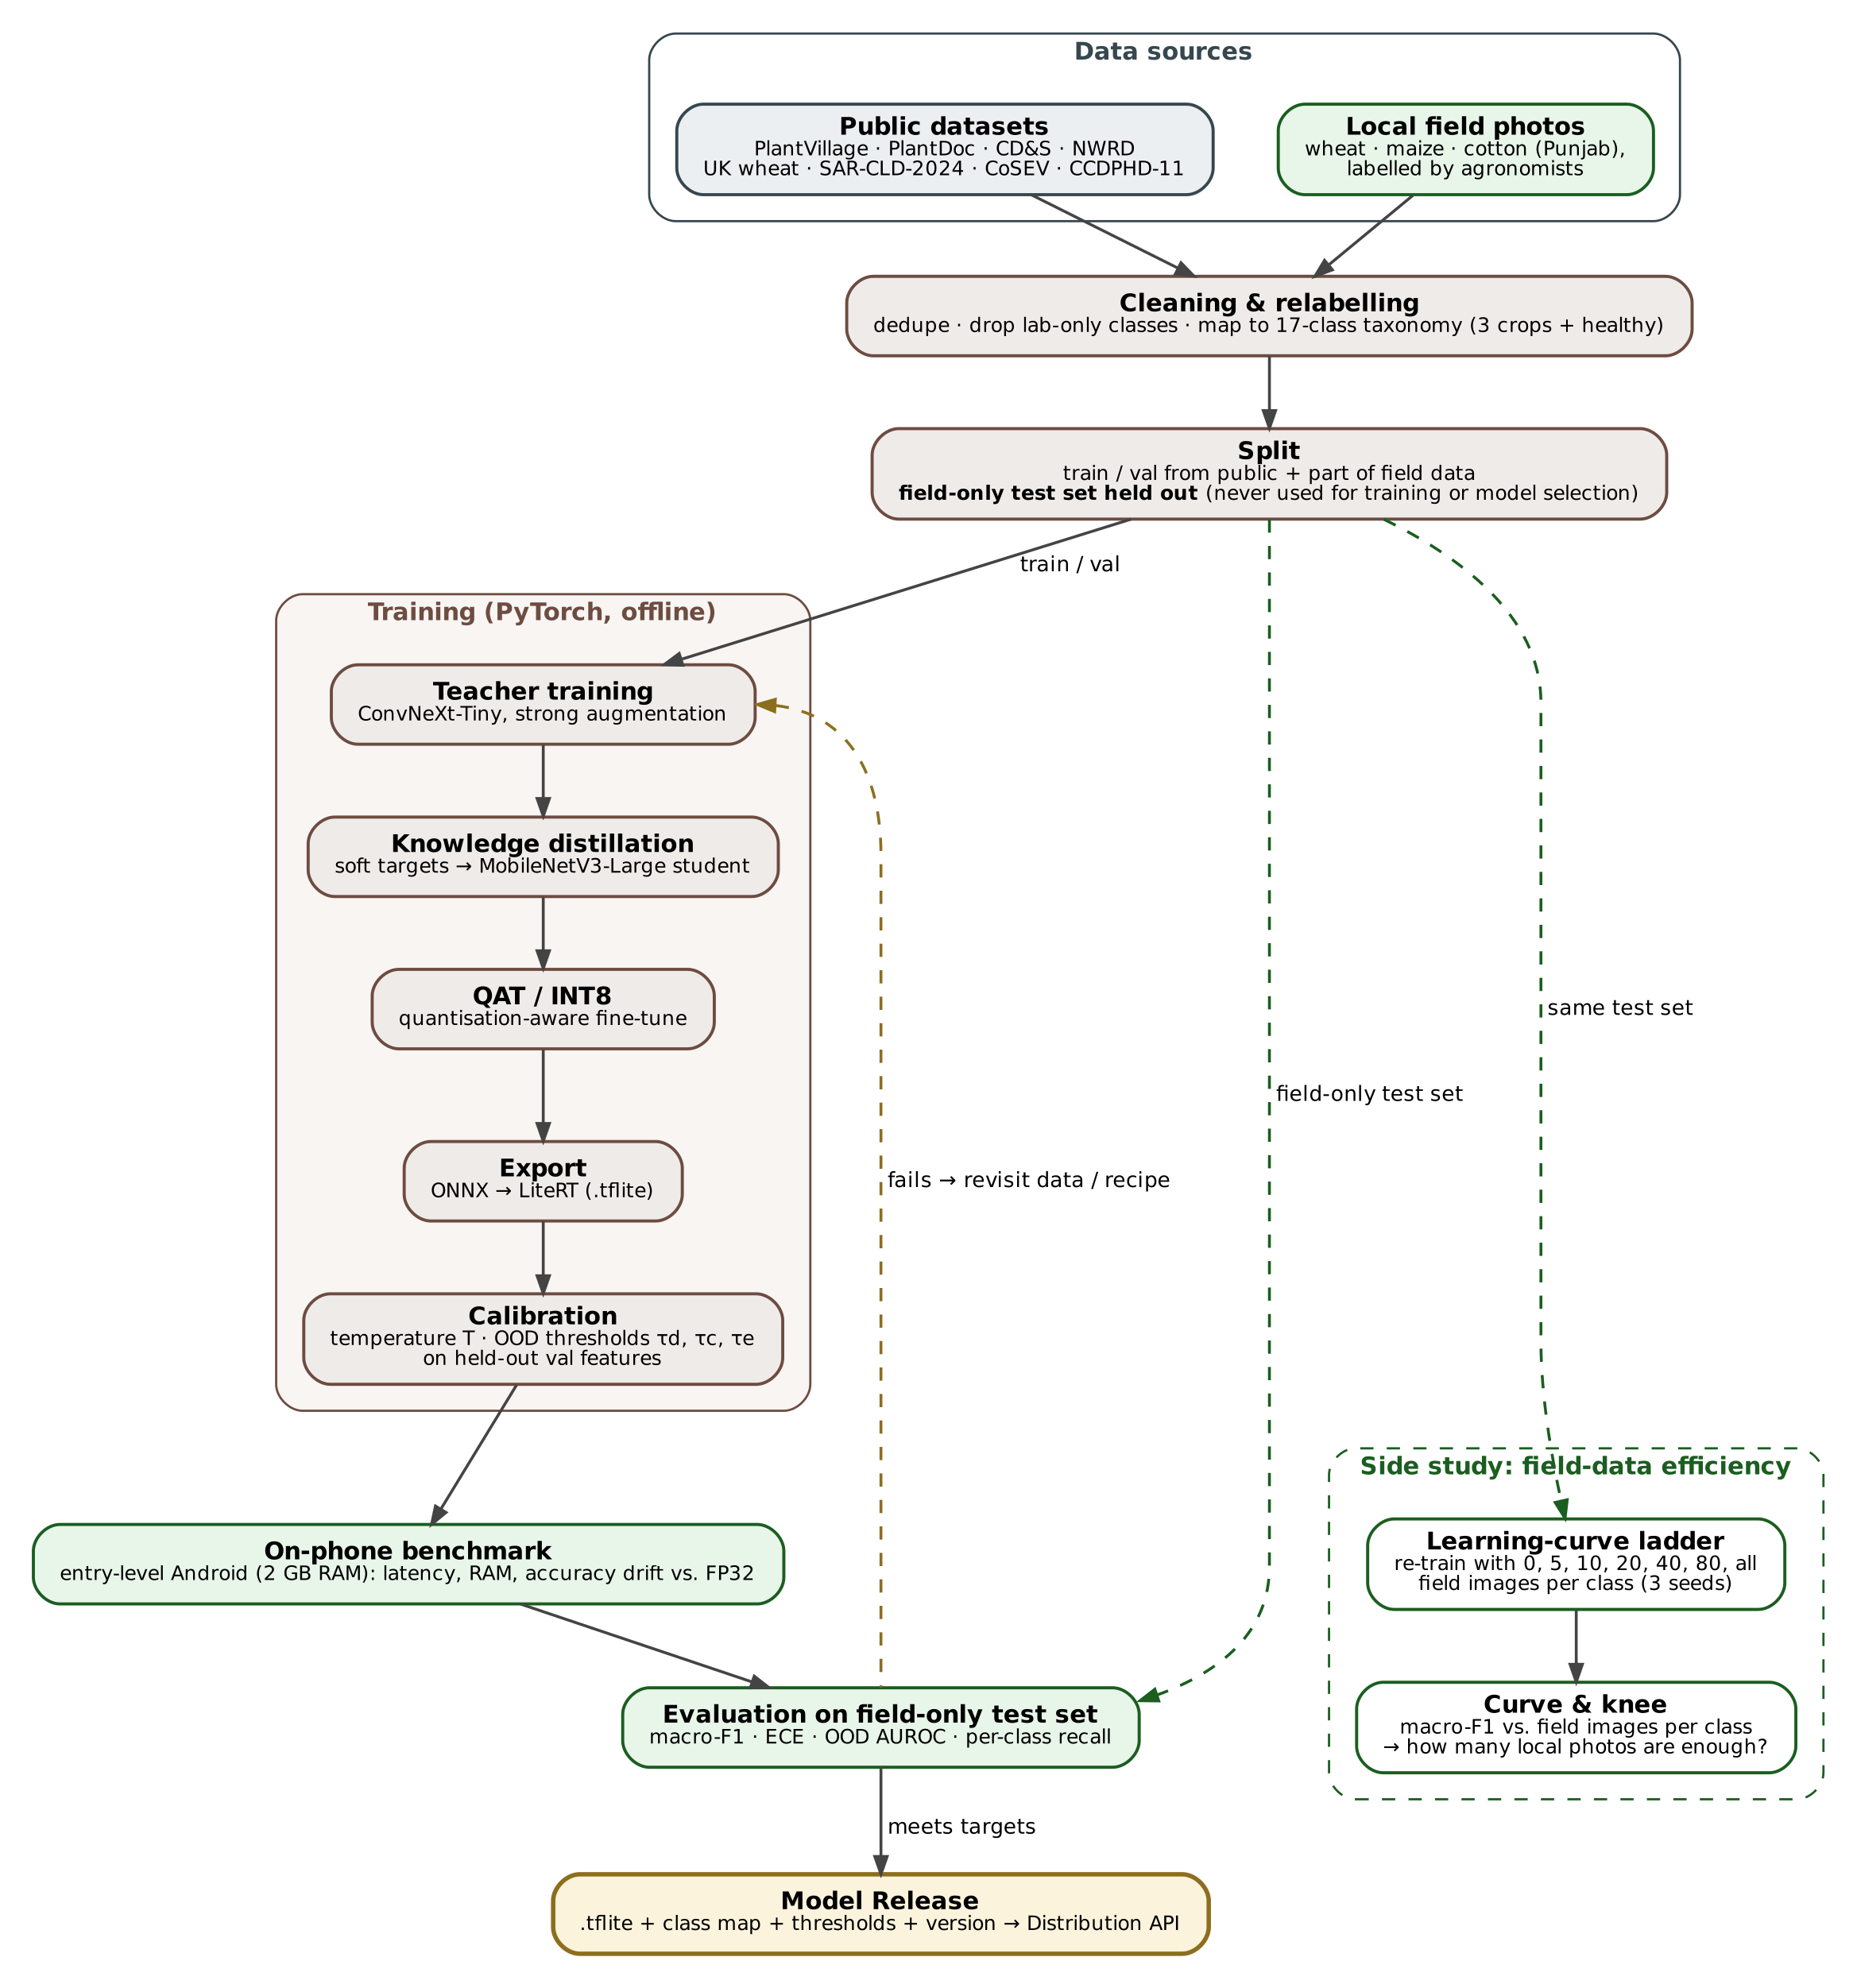
\includegraphics[width=\textwidth,height=0.88\textheight,keepaspectratio]{Figures/diagrams/pipeline_methodology.png}
  \caption{Training and deployment pipeline. Public datasets and local field photographs are mapped to the 17-class taxonomy; a field-only test set is held out; a larger teacher is trained and distilled into a MobileNetV3 student, which is quantised, exported, calibrated, benchmarked on entry-level phones and released. The field-data study branches from the same data.}
  \label{fig:pipeline}
\end{figure}

\section{Overview of the Approach}
Five principles, each drawn from the literature in Chapter~\ref{ch:lit}, guide the approach. We evaluate on field photographs, because that is where the application will be used. We train a large model and deploy a small one, using distillation and quantisation to keep most of the accuracy. We bring weather into the diagnosis as reviewed knowledge rather than as a learned input, because that needs no paired data and can be checked by agronomists. We check every input before answering, so that the app asks or declines rather than guesses. And we treat the amount of local data needed as a question to be measured rather than assumed.

\section{Data Strategy}
\label{sec:data}
\subsection{Taxonomy and sources}
All sources are mapped to the 17-class taxonomy of Table~\ref{tab:classes}; each source class maps to one KhetLens class or is left out, and the mapping is kept in a configuration file so the dataset can be rebuilt. Table~\ref{tab:datasets} lists the public sources we have identified. They come from several regions, which is a strength: variety in background, lighting and camera helps the model generalise. Local field photographs collected with our partner complete the picture for Punjab's conditions.

\begin{table}[H]
\centering\small
\caption{Public image sources mapped to the taxonomy.}
\label{tab:datasets}
\begin{tabularx}{\textwidth}{|L{3.6cm}|L{1.4cm}|L{2.6cm}|Y|}
\hline
\textbf{Source} & \textbf{Crop} & \textbf{Setting} & \textbf{Classes used} \\ \hline
PlantVillage~\cite{hughes2015plantvillage} & Maize & Laboratory & NLB, common rust, GLS, healthy \\ \hline
PlantDoc~\cite{singh2020plantdoc} & Maize & Field & NLB, rust, GLS \\ \hline
CD\&S~\cite{ahmad2021cds} & Maize & Field & NLB, GLS \\ \hline
NWRD~\cite{anwar2023nwrd} & Wheat & Field, Pakistan & Yellow (stripe) rust \\ \hline
Wheat field set~\cite{long2024ukwheat} & Wheat & Field and glasshouse & Yellow rust, brown rust, powdery mildew, Septoria leaf blotch (mapped to leaf blight), healthy \\ \hline
Punjab/KP wheat~\cite{malik2025wheatpk} & Wheat & Field and lab, Pakistan & Yellow and brown rust, powdery mildew, healthy \\ \hline
SAR-CLD-2024~\cite{sarcld2024} & Cotton & Field & Bacterial blight, leaf curl, reddening, leaf-hopper damage, healthy (subset of its seven classes) \\ \hline
CoSEV~\cite{noon2023cosev} & Cotton & Field, Pakistan & Leaf curl virus \\ \hline
CCDPHD-11~\cite{wang2025cotton} & Cotton & Mixed (online and field) & Bacterial blight, leaf curl, reddening, target spot (fungal leaf spot), pest damage, healthy \\ \hline
Pakistani cotton set~\cite{anwarcotton2023pk} & Cotton & Field and web & Healthy, bacterial blight, leaf curl \\ \hline
PlantWild~\cite{wei2024plantwild} & Various & In the wild & Plant-domain pre-training; non-target crops for OOD tests \\ \hline
\end{tabularx}
\end{table}

\subsection{Local field collection}
We collect photographs with our partner's field officers during the wheat season (winter) and the maize and cotton season (summer), using the same class of phone farmers own, under the lighting and backgrounds found at the time of the visit, with several leaves per plant. Each photograph is tagged with crop, date, district and growth stage, and an agronomist assigns the label. A subset is labelled by a second agronomist so that we can measure agreement. Unlabelled photographs are kept for self-supervised pre-training, and photographs of non-target crops and non-leaf scenes are collected as out-of-distribution test material.

\subsection{Splits and pre-processing}
We keep three disjoint sets. The training pool contains the public data plus the local photographs released to training. A validation set, stratified from the pool, is used for early stopping, temperature fitting and threshold selection. The field test set contains only local field photographs, split by plant so that no leaf of the same plant appears in both training and test, and is never used for tuning. Images are resized to 224 pixels for training with random crops at a range of scales, flips, colour jitter bounded to preserve lesion colour, and photometric distortions that imitate phone cameras (re-compression, mild blur, exposure shifts). To reduce background shortcuts, laboratory images are also composited onto field backgrounds. Class imbalance is handled by balanced sampling.

\section{Model Architecture}
\label{sec:model}
The deployed model is one network with a shared backbone and several heads, following the crop-conditional design that improved field accuracy in Picon et al.~\cite{picon2019cropcond}:
\begin{itemize}
  \item \textbf{Backbone:} MobileNetV3-Large~\cite{howard2019mnv3}, pre-trained on ImageNet and, where it helps, further pre-trained on plant images. It produces a feature vector $f(x)$ for the image.
  \item \textbf{Crop head:} three outputs (wheat, maize, cotton).
  \item \textbf{Disease heads:} one per crop with 6, 5 and 6 outputs; at inference only the head of the detected (or farmer-confirmed) crop is read.
\end{itemize}
The heads are trained together, each disease head receiving gradient only from images of its crop. We use an additive-margin softmax loss rather than plain cross-entropy, because margin losses make class clusters tighter and help the unknown-disease check~\cite{meng2023osr}. MobileNetV3-Small, EfficientNet-Lite and a MobileViT-class hybrid~\cite{tonmoy2025mobileplantvit} are trained with the same heads as benchmarked alternatives.

\subsection{Close-up and wider photographs}
\label{sec:multiscale}
Farmers will not always photograph a single leaf; many will photograph the affected plant from a short distance, with several leaves and part of the crop in view. We handle both kinds of photograph with the same model in two ways. During training, the images from field datasets already include a range of distances, and we add scale augmentation (random crops covering from a small part to the whole image) so that the model sees symptoms at different sizes. At inference, the photograph is classified as a whole and also as a small grid of overlapping regions; each region's probabilities are weighted by how confident the model is about it and averaged with the whole-image result. For a close-up this reduces to the ordinary single prediction; for a wider shot it lets the regions that contain affected leaves carry the decision. This adds only a few extra passes of the compact model and keeps the response time within our target.

\section{Training by Knowledge Distillation}
\label{sec:kd}
We first train a larger \emph{teacher} (ConvNeXt-Tiny, with the same head structure) on the training pool. The \emph{student} is then trained to match both the labels and the teacher's softened outputs~\cite{hinton2015kd}:
\begin{equation}
\mathcal{L}_{\text{KD}} = (1-\alpha)\,\mathcal{L}\big(y, \sigma(z_s)\big) + \alpha\, T_{\text{KD}}^2\, \mathrm{KL}\!\left( \sigma\!\left(\tfrac{z_t}{T_{\text{KD}}}\right) \,\middle\|\, \sigma\!\left(\tfrac{z_s}{T_{\text{KD}}}\right) \right),
\label{eq:kd}
\end{equation}
where $z_t$ and $z_s$ are the teacher's and student's logits, $\sigma$ is the softmax, $T_{\text{KD}}$ is the distillation temperature and $\alpha$ weights the two terms; both are chosen on the validation set. The value $\mathcal{L}_{\text{KD}}$ is the training loss we minimise: its first term measures how far the student's prediction is from the true label, its second how far the student's softened output is from the teacher's, so a low value means the student both predicts correctly and reproduces the teacher's view of which classes resemble each other. We run each reported configuration with three random seeds and report the mean and spread.

\section{Compression and Deployment}
\label{sec:deploy}
After training, the student is fine-tuned briefly with quantisation-aware training so that weights and activations can be stored as 8-bit integers with little loss~\cite{krishnamoorthi2018quant}. The calibration data include field images in proportion. We record accuracy before and after quantisation, and a release is held back if the drop on the field test set is more than a small margin. The model is exported to ONNX and converted to a TensorFlow Lite flatbuffer with full integer quantisation; the same graph is also packaged for ONNX Runtime so that the two runtimes can be compared on the phone~\cite{zhangq2022mobilebench}. The release bundle contains the model, the class map, the input size, the calibration temperature, the statistics used by the novelty check, and the thresholds.

\textbf{On-device benchmark.} On entry-level Android phones, after a short warm-up, we time a few hundred inferences and record the median and 95th-percentile latency, start-up time, peak memory and battery use for each runtime and input size. These measurements guide the final choice of runtime and input size.

\section{Context-Aware Fusion}
\label{sec:fusion}
Figure~\ref{fig:fusion} illustrates the weather adjustment. Let $p(y \mid x)$ be the calibrated probability of each condition $y$ of the detected crop for image $x$, and let $w$ summarise the district's weather over the preceding two weeks: mean daily maximum and minimum temperature, mean relative humidity, total rainfall and days since rain. A \emph{plausibility prior} $\pi(y \mid w)$, between a floor $\pi_{\min}$ and 1, is read from a lookup table built from epidemiological literature and reviewed by agronomists. The adjusted result is
\begin{equation}
\tilde{p}(y \mid x, w) = \frac{p(y \mid x)\, \pi(y \mid w)^{\lambda}}{\sum_{y'} p(y' \mid x)\, \pi(y' \mid w)^{\lambda}},
\label{eq:fusion}
\end{equation}
where $\lambda \in [0,1]$ sets how strongly the weather is allowed to influence the result. The value $\tilde{p}(y \mid x, w)$ is the adjusted probability of each condition given both the photograph and the recent weather; the conditions still sum to one, and the condition with the highest $\tilde{p}$ is the one shown to the farmer. The floor $\pi_{\min}$ means the weather can make a condition less likely but never rule it out, and when no recent weather is stored the prior is uniform and the result screen says so.

\begin{figure}[H]
  \centering
  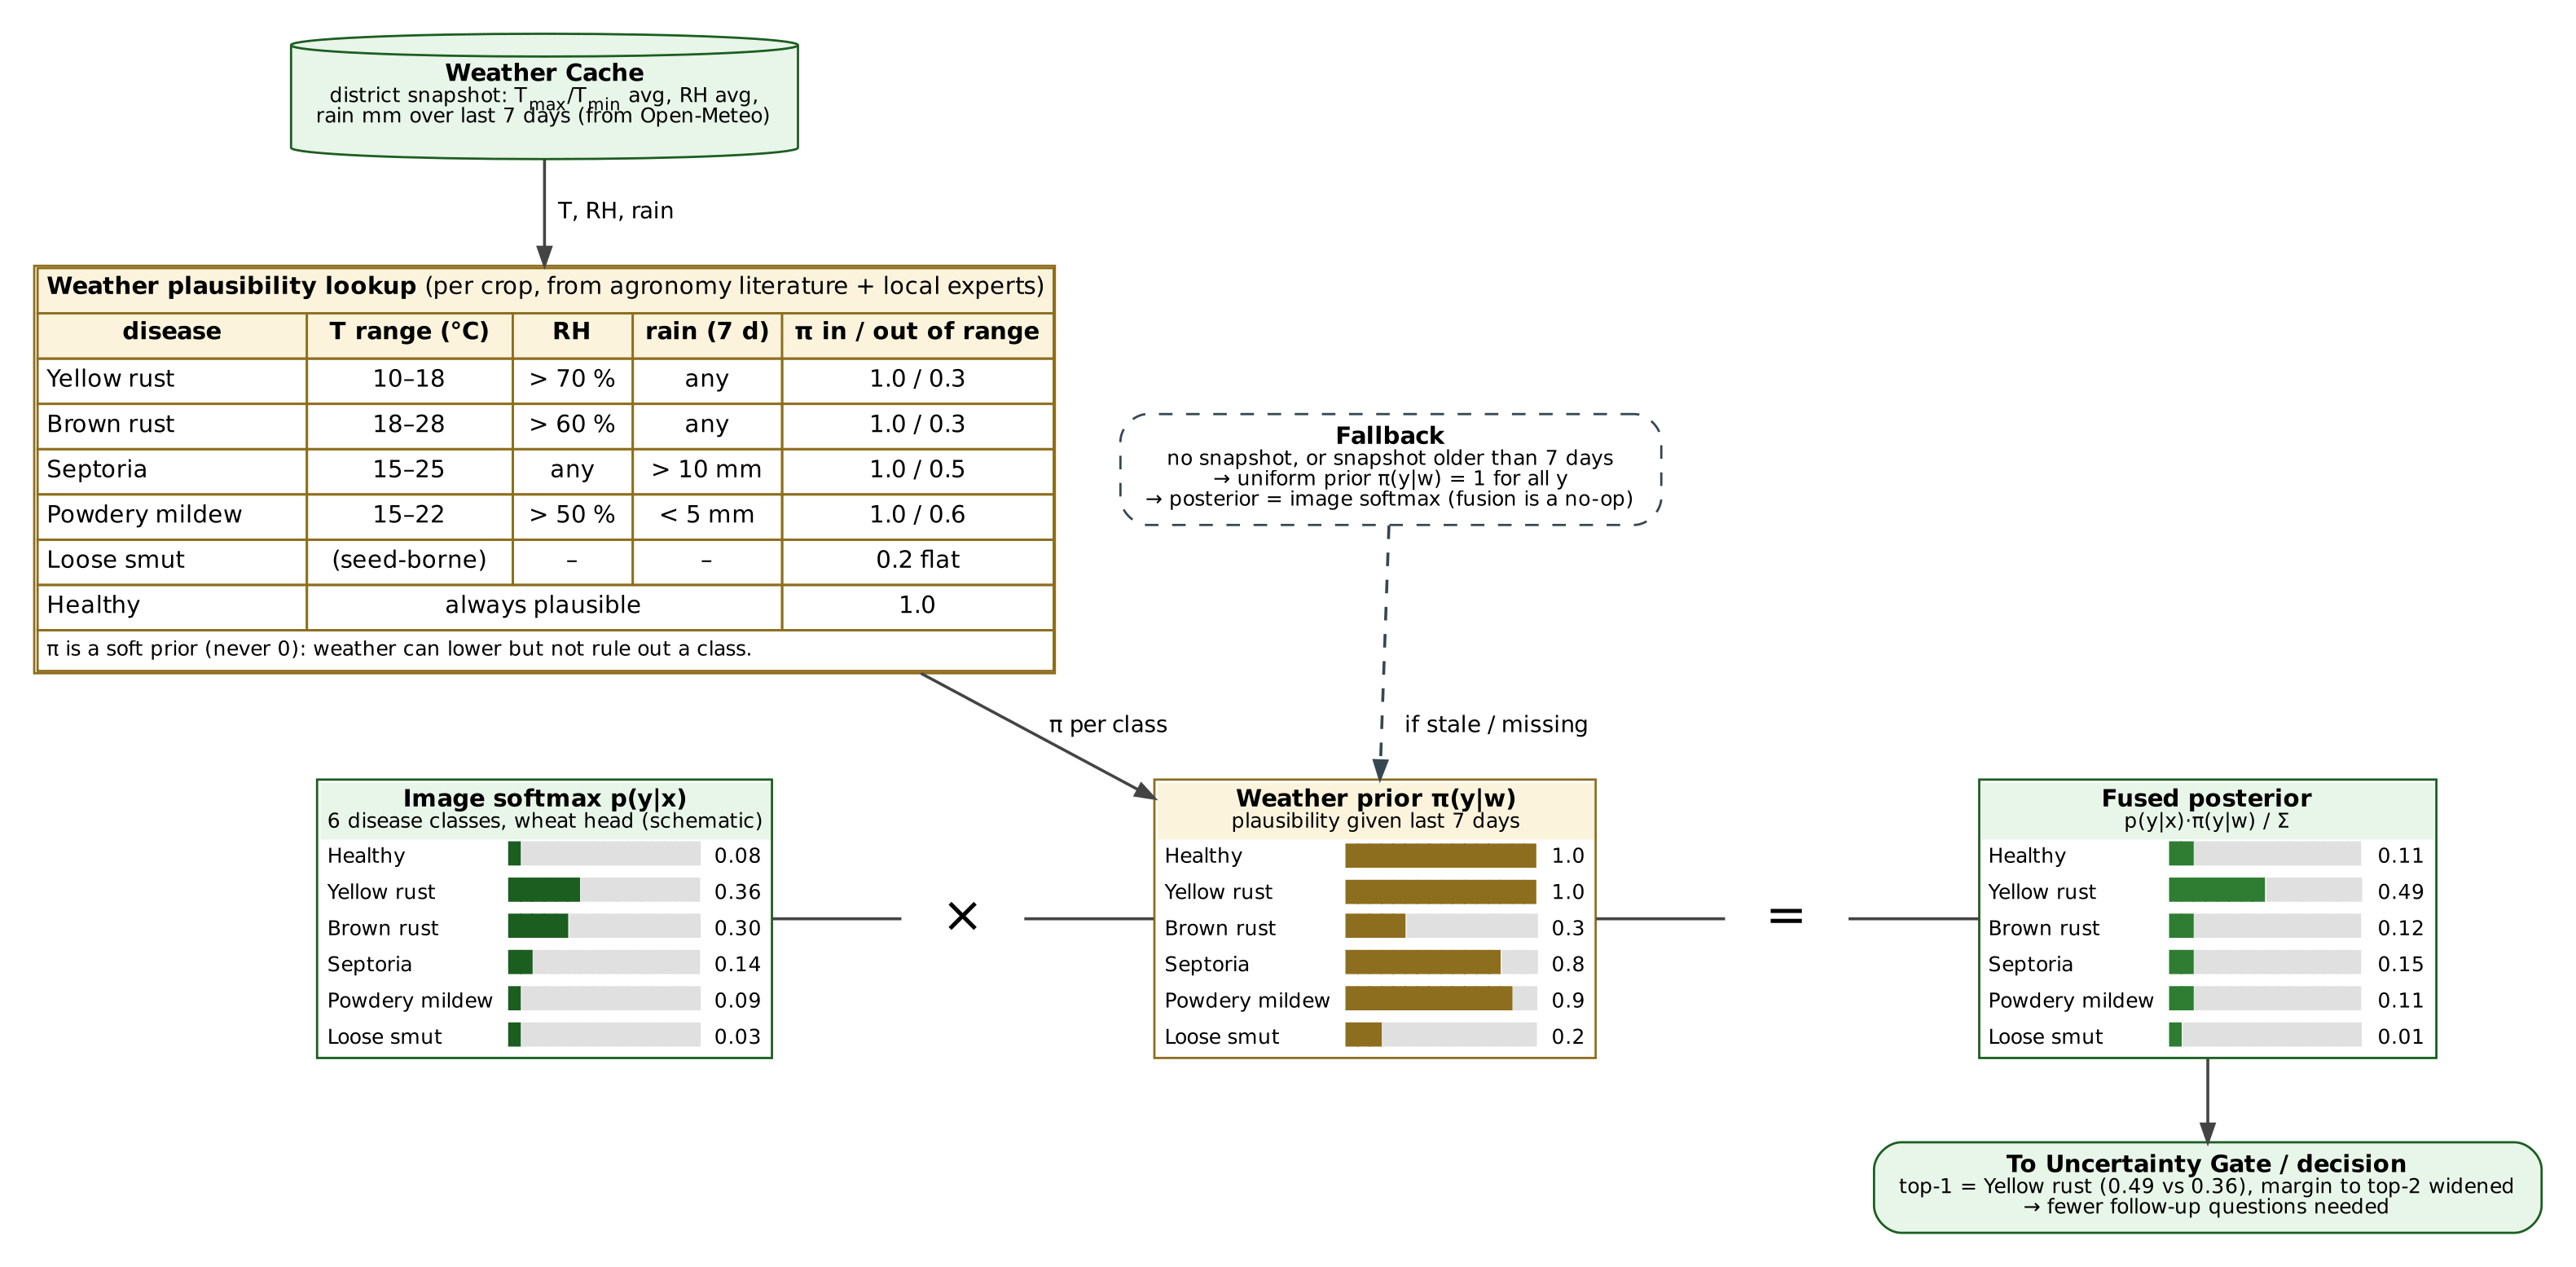
\includegraphics[width=\textwidth,height=0.88\textheight,keepaspectratio]{Figures/diagrams/fusion_diagram.png}
  \caption{Weather-aware adjustment (shown with $\lambda = 1$). The classifier's probabilities over the crop's conditions are multiplied by a plausibility prior read from a lookup table and renormalised. Bars are illustrative. When no recent weather is stored, the prior is uniform.}
  \label{fig:fusion}
\end{figure}

Table~\ref{tab:prior} gives an illustrative excerpt of the table for wheat. The stripe rust row uses the ranges fitted on Punjab data by Ali et al.~\cite{ali2023striperust}; the other rows are our initial proposals and will be set with the agronomists. The table is part of the content pack, so it can be refined without changing the model. The value of $\lambda$ is chosen on the validation set by looking at the designated look-alike pairs (Section~\ref{sec:pairs}), with the condition that no class loses accuracy, and the result with $\lambda = 0$ is always reported alongside.

\begin{table}[H]
\centering\small
\caption{Illustrative weather plausibility table for wheat (excerpt, to be set with agronomists).}
\label{tab:prior}
\begin{tabularx}{\textwidth}{|L{2.8cm}|Y|L{1.2cm}|}
\hline
\textbf{Condition} & \textbf{Rule on the two-week summary} & \textbf{$\pi$} \\ \hline
Yellow rust & Daily maxima mostly 13--23\,$^\circ$C and humidity 50--85\%~\cite{ali2023striperust} & 1.0 \\
 & One of the two holds & 0.7 \\
 & Neither holds (for example, hot and dry) & 0.3 \\ \hline
Powdery mildew & Humid with little rain & 1.0 \\
 & Otherwise & 0.6 \\ \hline
Leaf blight & Recent rain and warm & 1.0 \\
 & Otherwise & 0.6 \\ \hline
Abiotic stress & Hot spell or long dry period & 1.0 \\
 & Otherwise & 0.5 \\ \hline
Healthy & Always & 1.0 \\ \hline
\end{tabularx}
\end{table}

\section{Uncertainty Check and Follow-Up Questions}
\label{sec:gate}
Figure~\ref{fig:gate} shows the uncertainty check as a flowchart and Algorithm~\ref{algo:gate} gives the procedure. Three signals are computed from the model's outputs; for a wider photograph, the feature vector and logits used below are the combined whole-image and region results of Section~\ref{sec:multiscale}.

\begin{figure}[H]
  \centering
  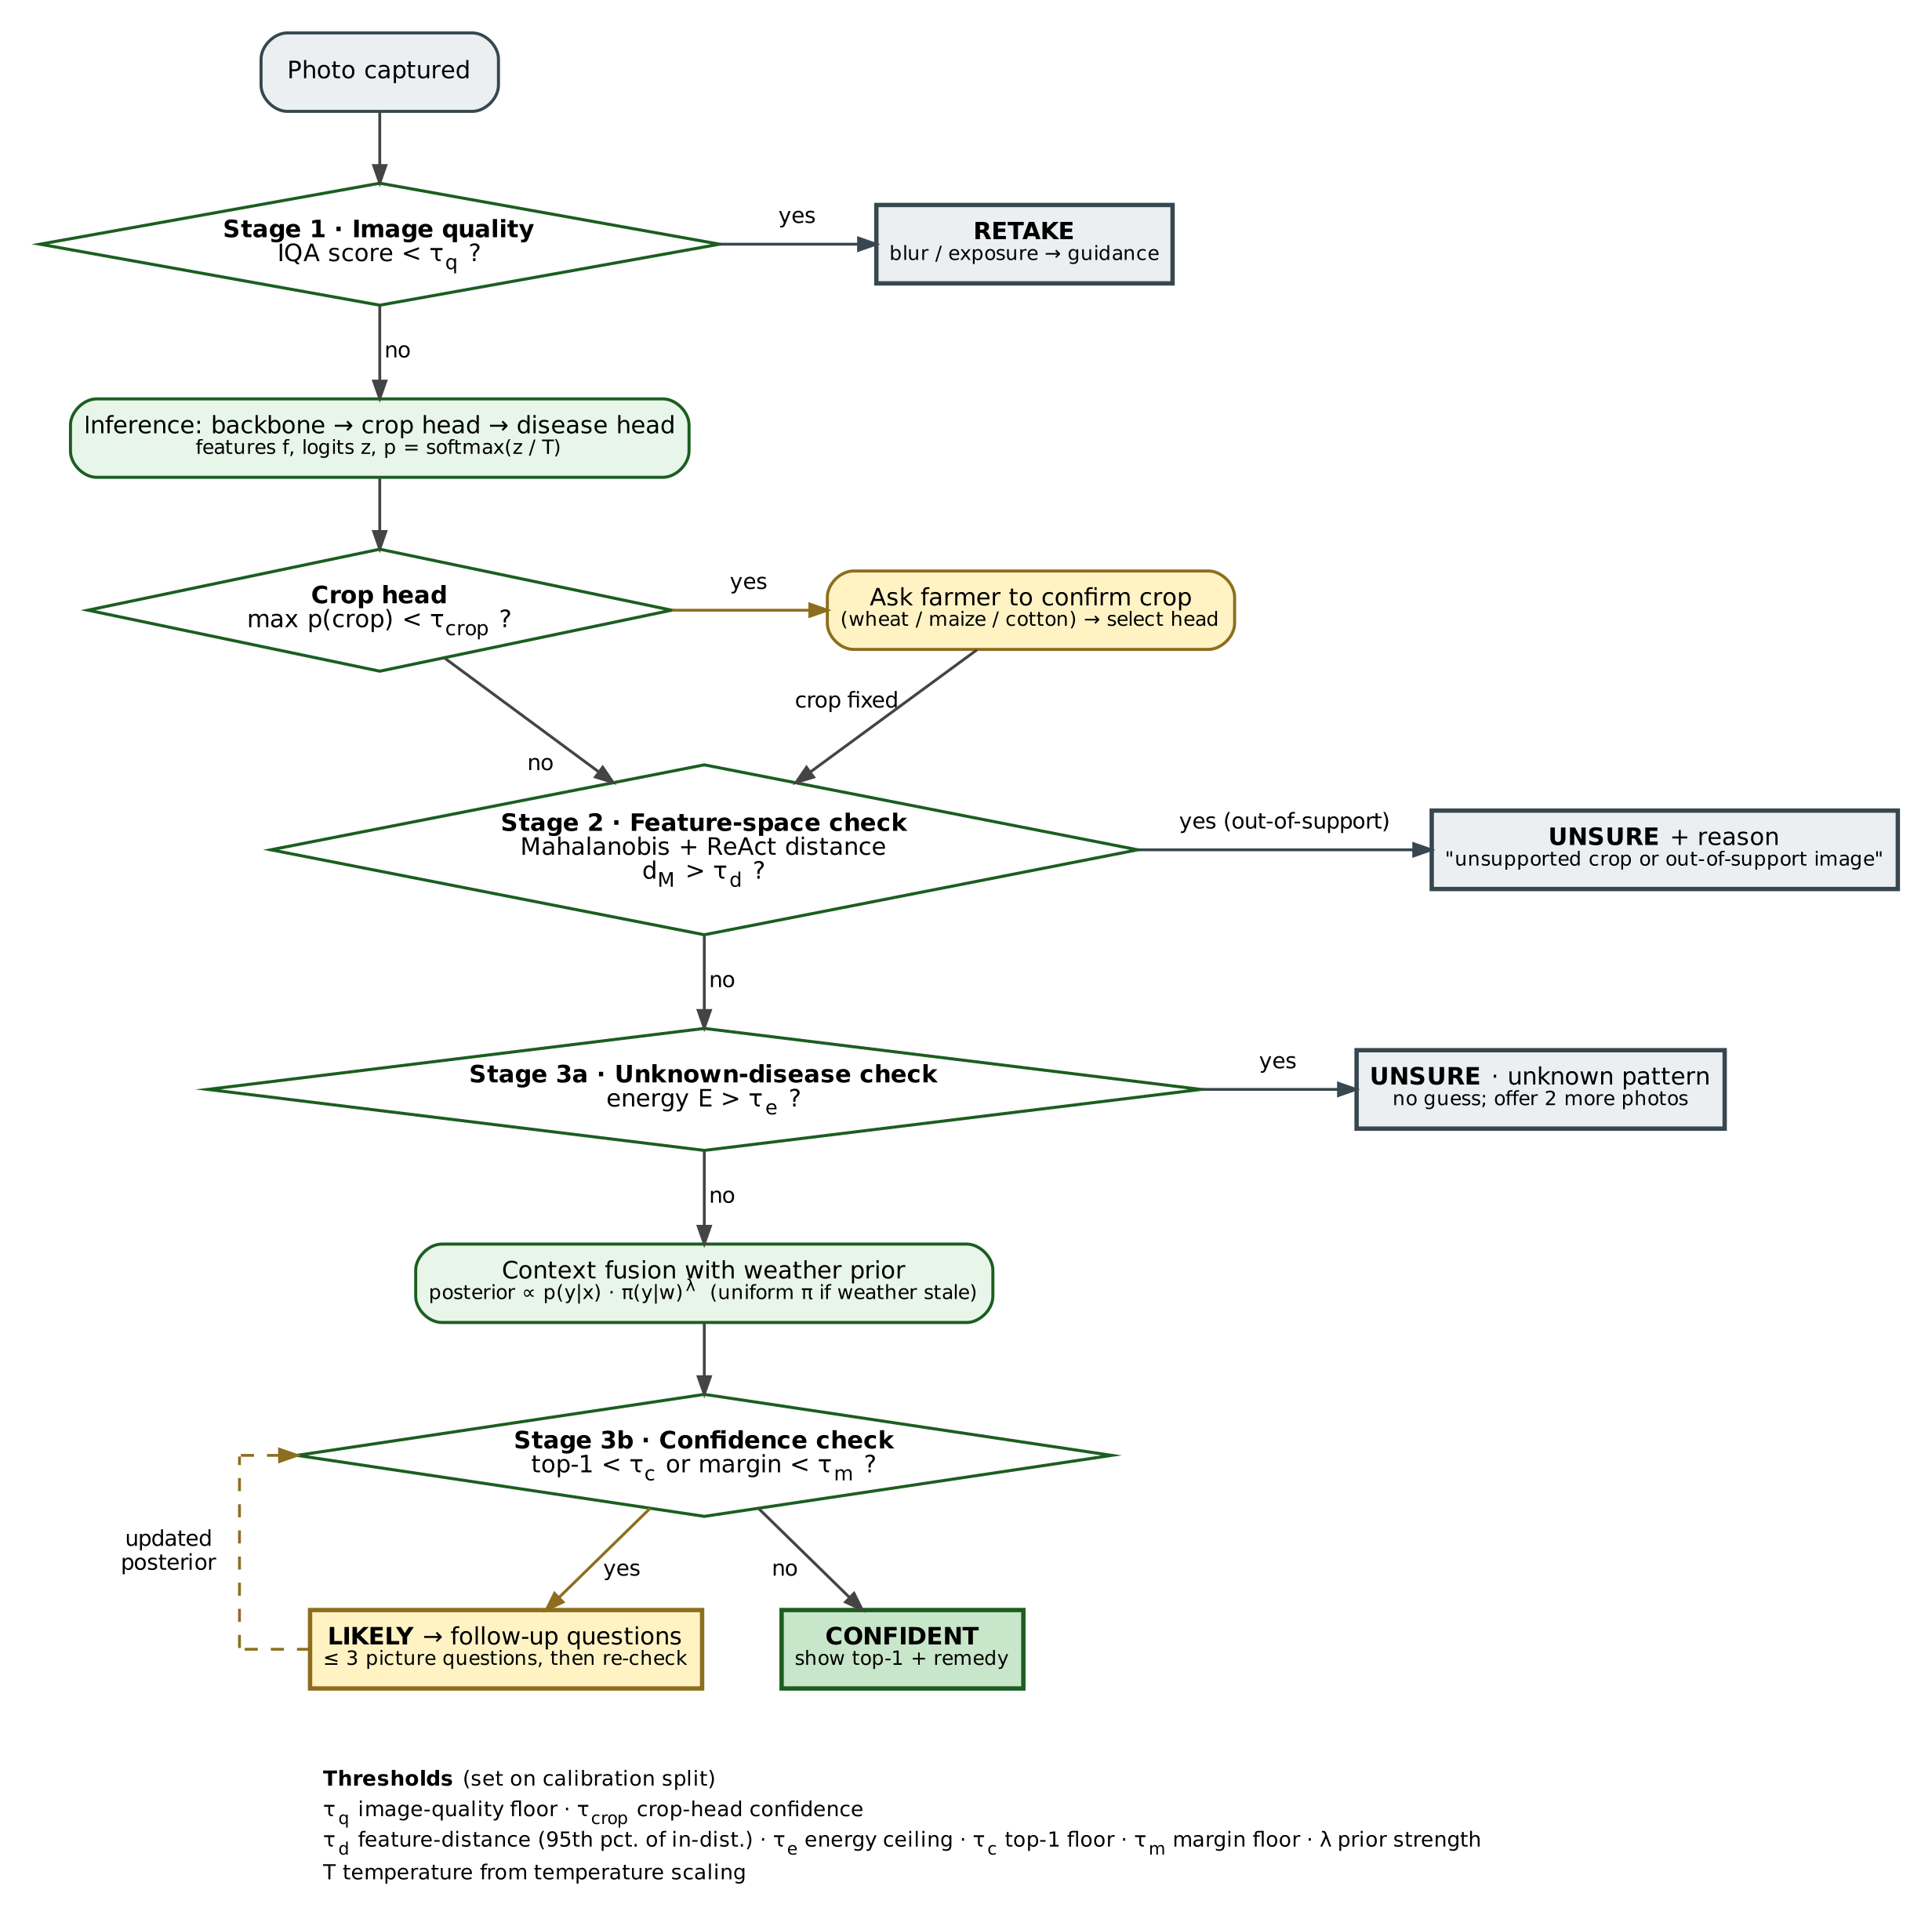
\includegraphics[width=\textwidth,height=0.88\textheight,keepaspectratio]{Figures/diagrams/gate_flowchart.png}
  \caption{The three-stage uncertainty check. Stage~1 rejects unusable photographs; Stage~2 recognises unsupported crops and other out-of-support images by feature distance; Stage~3a declines unfamiliar patterns by energy score before the weather adjustment, and Stage~3b sends low-confidence or near-tie results to follow-up questions after it. Thresholds are set on field data and shipped with the model.}
  \label{fig:gate}
\end{figure}

\textbf{Stage 1: image quality.} Before inference, a sharpness measure (variance of the Laplacian of the grey image) and an exposure measure (fraction of very dark or very bright pixels) are combined into a quality score, following the idea of a quality gate in AgroPath~\cite{ahmed2022agropath}. Below a threshold $\tau_q$ the photograph is sent back for a retake with the reason.

\textbf{Stage 2: feature-space novelty.} The backbone features are first clipped as in ReAct~\cite{sun2021react}, $f'(x) = \min(f(x), \kappa)$, and the Mahalanobis distance to the nearest class of the detected crop is then computed~\cite{lee2018mahalanobis}; combining the two is our own choice, and we will also evaluate the distance without clipping:
\begin{equation}
d_M(x) = \min_{k} \big(f'(x) - \mu_k\big)^{\!\top} \Sigma^{-1} \big(f'(x) - \mu_k\big),
\label{eq:maha}
\end{equation}
with class means $\mu_k$ and a shared covariance $\Sigma$ estimated on the training set and stored with the model. The value $d_M(x)$ measures how far the photograph's features lie from the nearest known class, scaled by how spread out that class normally is; a small value means the photograph looks like something the model was trained on, a large value means it does not. If $d_M(x)$ exceeds $\tau_d$ the input is treated as unsupported. Before this check, a crop-head confidence below $\tau_{crop}$ triggers a crop-confirmation prompt instead.

\textbf{Stage 3a: unknown-disease check.} The energy score $E(x) = -T \log \sum_k \exp(z_k / T)$~\cite{liu2020energy}, where $z_k$ are the logits of the crop's disease head and $T$ the calibration temperature, summarises how strongly the model responds to the image overall: a low (more negative) value means at least one class fired strongly, a high value means no class did, which is typical of an unfamiliar pattern. It is compared with the softmax baseline~\cite{hendrycks2017msp} during evaluation, and the better of the two on held-out diseases is shipped. Above its threshold $\tau_e$ the outcome is Unsure with reason ``unfamiliar pattern'', and the farmer is offered two more photographs. In Algorithm~\ref{algo:gate} this score is written as $E$; if the softmax score wins the comparison it takes the same place.

\textbf{Stage 3b: calibrated confidence.} Logits are temperature-scaled~\cite{guo2017calibration}, $p = \sigma(z/T)$, with $T$ fitted on the validation set; the resulting $p$ is a probability for each condition whose value matches how often the model is actually right at that level, so that ``87\%'' on the result screen means roughly 87 in 100 such results are correct. After the weather adjustment, if the top probability is at least $\tau_c$ and the margin over the second is at least $\tau_m$, the outcome is Confident; otherwise it is Likely and the follow-up questions begin.

Thresholds are set on the validation set: $\tau_q$ to send most blurred photographs for retake while rarely rejecting sharp ones; $\tau_{crop}$ to ask for crop confirmation only when the crop head is genuinely unsure; $\tau_d$ and $\tau_e$ to keep nearly all supported inputs while rejecting as many out-of-support inputs as possible, tested against non-leaf images, leaves of other crops and held-out diseases; $\tau_c$ and $\tau_m$ to keep accuracy high on the results marked Confident. All thresholds ship in the model release and are re-fitted for each release.

\begin{algorithm}[H]
\small
\KwData{image $x$; weather summary $w$ (may be absent); model; release parameters $T, \mu, \Sigma^{-1}, \kappa, \tau_q, \tau_{crop}, \tau_d, \tau_e, \tau_c, \tau_m, \lambda$}
\KwResult{one of \textsc{Retake}, \textsc{ConfirmCrop}, \textsc{Confident}, \textsc{Likely}, \textsc{Unsure}}
$q \leftarrow \textsc{QualityScore}(x)$\;
\If{$q < \tau_q$}{\Return \textsc{Retake}(reason)\;}
$f \leftarrow \textsc{Backbone}(x)$; \quad $p_{crop} \leftarrow \sigma(\textsc{CropHead}(f))$\;
\If{$\max p_{crop} < \tau_{crop}$}{\Return \textsc{ConfirmCrop}($p_{crop}$)\;}
$c \leftarrow \arg\max p_{crop}$; \quad $z \leftarrow \textsc{DiseaseHead}_{c}(f)$\;
$d_M \leftarrow$ Equation~\ref{eq:maha} on $\min(f, \kappa)$\;
\If{$d_M > \tau_d$}{\Return \textsc{Unsure}(``unsupported'')\;}
$p \leftarrow \sigma(z / T)$; \quad $E \leftarrow -T\log\sum_k \exp(z_k/T)$\;
\If{$E > \tau_e$}{\Return \textsc{Unsure}(``unfamiliar pattern'')\;}
$\pi \leftarrow$ recent $w$ available ? \textsc{PriorTable}$(c, w)$ : uniform\;
$\tilde{p} \leftarrow p \odot \pi^{\lambda} / \sum (p \odot \pi^{\lambda})$\;
\eIf{$\tilde{p}_{(1)} \geq \tau_c \ \wedge\ \tilde{p}_{(1)} - \tilde{p}_{(2)} \geq \tau_m$}{
  \Return \textsc{Confident}($\arg\max \tilde{p}$, $\tilde{p}_{(1)}$, reasons)\;
}{
  \Return \textsc{Likely}(top two of $\tilde{p}$)\;
}
\caption{Diagnosis with the uncertainty check and weather adjustment.}
\label{algo:gate}
\end{algorithm}

\textbf{Follow-up questions.} For a Likely outcome, the app loads the crop's question set from the content pack. Each question has two or three illustrated options, and for each option and condition the pack stores a likelihood set by the agronomists on a coarse scale (typical, neutral, unlikely). After each answer the probabilities are updated by Bayes' rule, and ``Not sure'' leaves them unchanged. The next question is the one that best separates the remaining candidates, and the dialogue stops as soon as one condition dominates or after three questions, when the outcome becomes Unsure. This follows the conversational approach of DSSApple~\cite{sottocornola2022dssapple}. The ``take two more photos'' step averages the adjusted probabilities of all photographs that pass the first two stages and re-applies the third, following the multi-leaf finding of the Nuru field study~\cite{mrisho2020nuru}.

\section{Field-Data Efficiency Study}
\label{sec:study}
This study answers RQ2 with a learning-curve experiment; Figure~\ref{fig:study} shows the expected shape.

\begin{figure}[H]
  \centering
  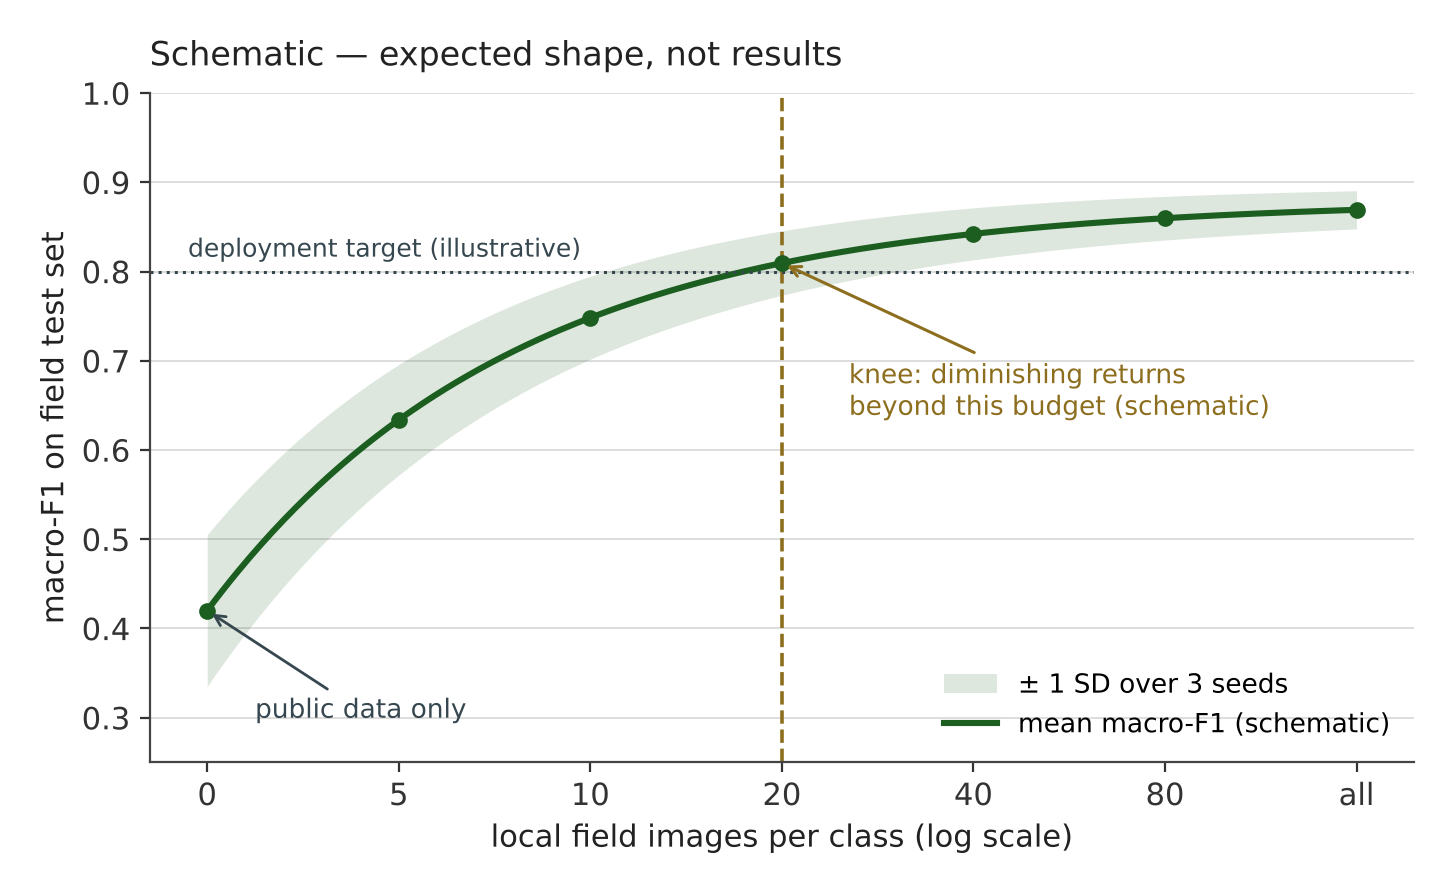
\includegraphics[width=\textwidth,height=0.88\textheight,keepaspectratio]{Figures/diagrams/study_design.png}
  \caption{Design of the field-data efficiency study (expected shape, not results). Macro-F1 on the fixed field test set is plotted against the number of local field images per class released to training; the band shows the spread across seeds and the knee marks diminishing returns.}
  \label{fig:study}
\end{figure}

The field test set is fixed first and never touched. For each point on a logarithmic ladder of local images per class (0, 5, 10, 20, 40, 80, and all available), and for each of three random seeds, a random subset of that size is added to the public training pool and the student is fine-tuned from the public-only checkpoint. The ladder matches the few-shot grids in the literature~\cite{argueso2020fewshot,xu2022transfer} so that our results can be compared with them. We report macro-F1 and per-class F1 on the field test set as mean and spread over seeds, per crop and overall, fit the power law $\text{err}(N) = a\,N^{\gamma} + \varepsilon_\infty$~\cite{beck2022curves}, where $\text{err}(N)$ is the error on the field test set after adding $N$ local images per class, $\gamma$ (negative) is how quickly error falls as data grows, $\varepsilon_\infty$ is the error that remains however much data is added, and $a$ is a scale constant; and report the knee as the smallest $N$ beyond which doubling the local data gains less than one point. Two secondary comparisons are run alongside: with and without self-supervised pre-training on the unlabelled local photographs, and random against uncertainty-based selection of which images to label. Each fine-tuning run is short enough that the full ladder fits within our compute allocation.

\section{Evaluation Plan}
\label{sec:eval}
Table~\ref{tab:evalplan} maps the research questions and objectives to experiments and metrics. All classification metrics are computed on the field test set; accuracy on laboratory images is reported only to show the size of the gap.

\begin{table}[H]
\centering\small
\caption{Evaluation plan.}
\label{tab:evalplan}
\begin{tabularx}{\textwidth}{|L{1.4cm}|Y|L{3.6cm}|}
\hline
\textbf{Question} & \textbf{Experiment} & \textbf{Metrics} \\ \hline
RQ1 & Train on public data; test on laboratory split, held-out public field sets and the local field test set; with and without background augmentation; teacher vs student vs quantised student. & Accuracy, macro-F1, per-class F1 \\ \hline
RQ2 & Learning-curve ladder (Section~\ref{sec:study}). & Macro-F1 against $N$, fitted curve, knee \\ \hline
RQ3 & Weather adjustment on and off; confusion on the look-alike pairs; behaviour with missing weather. & Macro-F1 on pairs, per-class change \\ \hline
RQ4 & Softmax vs energy vs Mahalanobis on three OOD sets; calibration before and after temperature scaling; quality check on degraded images. & AUROC, false-positive rate at 95\% recall, calibration error, retake rate \\ \hline
O2 & On-device benchmark (Section~\ref{sec:deploy}). & Latency, start-up, memory, battery \\ \hline
O6 & Task-based test with farmers through our partner. & Task completion, time, feedback \\ \hline
\end{tabularx}
\end{table}

\textbf{Ethics.} Field photograph collection and farmer testing follow a protocol agreed with our supervisor and shared with our partner: oral consent in the participant's language, voluntary participation, no capture of faces, photographs stored only on team systems, and results reported in aggregate. Server-side records hold a hashed phone number and the district only.

\section{Conclusion}
This chapter has set out our approach in enough detail to be reproduced: the sources and their mapping to the taxonomy, the field-collection protocol, a shared-backbone multi-head MobileNetV3 student distilled from a larger teacher, quantisation-aware compression with a release check, an on-device benchmark, a reviewable weather adjustment with a floor and a fallback, a three-stage uncertainty check with follow-up questions, and a seeded learning-curve study. Each choice is tied to a finding in Chapter~\ref{ch:lit} and each research question to an experiment. The next chapter describes the software that carries this core to the farmer.

\chapter{High-Level and Low-Level Design}
\label{ch:design}

This chapter presents the design of the KhetLens software: the system as a whole, the considerations that shaped it, the architecture and its subsystems, the main design strategies and the alternatives we considered, the class structure of the mobile application, the sequence of interactions for the main use cases, and the policies we follow in implementation. The design realises the requirements of Chapter~\ref{ch:srs} and carries the diagnostic core of Chapter~\ref{ch:method} to the farmer's phone.

\section{System Overview}
KhetLens has four parts (Figure~\ref{fig:arch}). The \textbf{mobile application}, written in Kotlin, holds all farmer-facing functionality and is designed so that every use case works without a network: it captures and checks the photograph, runs the quantised model, applies the uncertainty check and the weather adjustment, drives the follow-up questions, looks up guidance in the local content pack, plays audio, and stores history and feedback locally. The \textbf{KhetLens server}, a small FastAPI service on PostgreSQL, has few responsibilities: one-time verification, feedback collection, distribution of model and content updates, and aggregate analytics. Two \textbf{external services} are used: a weather API, called by the phone when it is connected, and a WhatsApp-based one-time code service, called by the server. The \textbf{training pipeline} is an offline Python system that produces model releases; its outputs (model, class map, thresholds, novelty statistics) are consumed by the app.

The design approach can be summed up as \emph{offline-first, local-compute, data-as-content}. Everything a farmer needs is on the phone; the network is used opportunistically; and everything an agronomist might want to change (disease entries, guidance, questions, the weather table, audio) is data in a versioned content pack rather than code.

\section{Design Considerations}
The design is shaped by what the system may assume, the constraints it must respect, the principles we chose to follow, and our development method.

\subsection{Assumptions and Dependencies}
\begin{itemize}
  \item \textbf{Platform:} Android 8.1 or later on entry-level phones; CPU-only inference; camera and GPS present. The app depends on the standard Android libraries, the TensorFlow Lite runtime and Kotlin coroutines.
  \item \textbf{Model contract:} the app depends on a model release with a fixed interface: an image tensor in, and the backbone features, crop logits and per-crop disease logits out, with a manifest giving the class map, input size and thresholds. Any model that follows the contract can be swapped in.
  \item \textbf{Content contract:} the app depends on a content pack that follows a JSON schema (conditions, guidance, questions, weather table, audio list), validated at publish time.
  \item \textbf{Users:} farmers who may not read and use the phone one-handed outdoors; field officers who install and demonstrate the app; agronomists who review content offline.
  \item \textbf{Likely changes:} the disease list will be refined after agronomist review (handled by per-crop heads and the class map); the weather provider may change (handled by an interface); more crops may be added later (handled by the head structure and content schema).
\end{itemize}

\subsection{General Constraints}
\begin{itemize}
  \item \textbf{Memory and compute:} a few gigabytes of RAM shared with the system; inference must complete in about two seconds on an entry-level CPU (NFR-01).
  \item \textbf{Network:} absent or intermittent; no farmer action may wait on it; all network work is deferrable and safe to retry (NFR-03).
  \item \textbf{Storage:} total install under 150\,MB (NFR-02); photographs stored at reduced resolution; audio compressed; history kept for six months; feedback removed from the phone once uploaded.
  \item \textbf{Security and privacy:} tokens in encrypted storage; TLS everywhere; photographs and GPS never uploaded without opt-in (NFR-08).
  \item \textbf{Standards:} Android accessibility guidelines for tap targets and contrast; correct bidirectional layout for Urdu and Punjabi.
\end{itemize}

\subsection{Goals and Guidelines}
\begin{itemize}
  \item \textbf{Offline-first.} Design every feature as if the network did not exist, then add synchronisation.
  \item \textbf{Never block the farmer.} Background work runs in deferred jobs and never shows a spinner on a farmer-facing screen.
  \item \textbf{Honesty over coverage.} A ``not sure'' outcome is a correct output with its own screen and actions, not an error.
  \item \textbf{Data over code.} Anything an agronomist might change is content, validated and hot-swappable.
  \item \textbf{Measure on real phones.} Latency and memory claims come from entry-level devices, not emulators.
  \item \textbf{Keep the backend small.} The server does nothing the phone could do.
  \item \textbf{Separate ML from UI.} The ML layer exposes a plain Kotlin interface so the model and the app can be developed and tested independently.
\end{itemize}

\subsection{Development Methods}
We follow an Agile process with two-week sprints, a backlog in GitHub Issues, pull requests reviewed by a second team member and automated checks on each change. Each sprint ends with a demonstration to our supervisor. Training runs are tracked with their configuration, data version and seeds so that results can be regenerated. The app follows the layered architecture common in Android (presentation, domain, data) with the ML components as a separate module, and the MVVM pattern in the presentation layer. We considered Flutter for the app and chose native Android because the inference runtime, camera control and Nastaliq text rendering are all first-class there and the project is Android-only by scope.

\section{System Architecture}
Figure~\ref{fig:arch} shows the high-level architecture. The dashed boundary around the phone marks the offline-capable region: every arrow inside it works without a network, and every arrow crossing it is marked ``when connected''.

\begin{figure}[H]
  \centering
  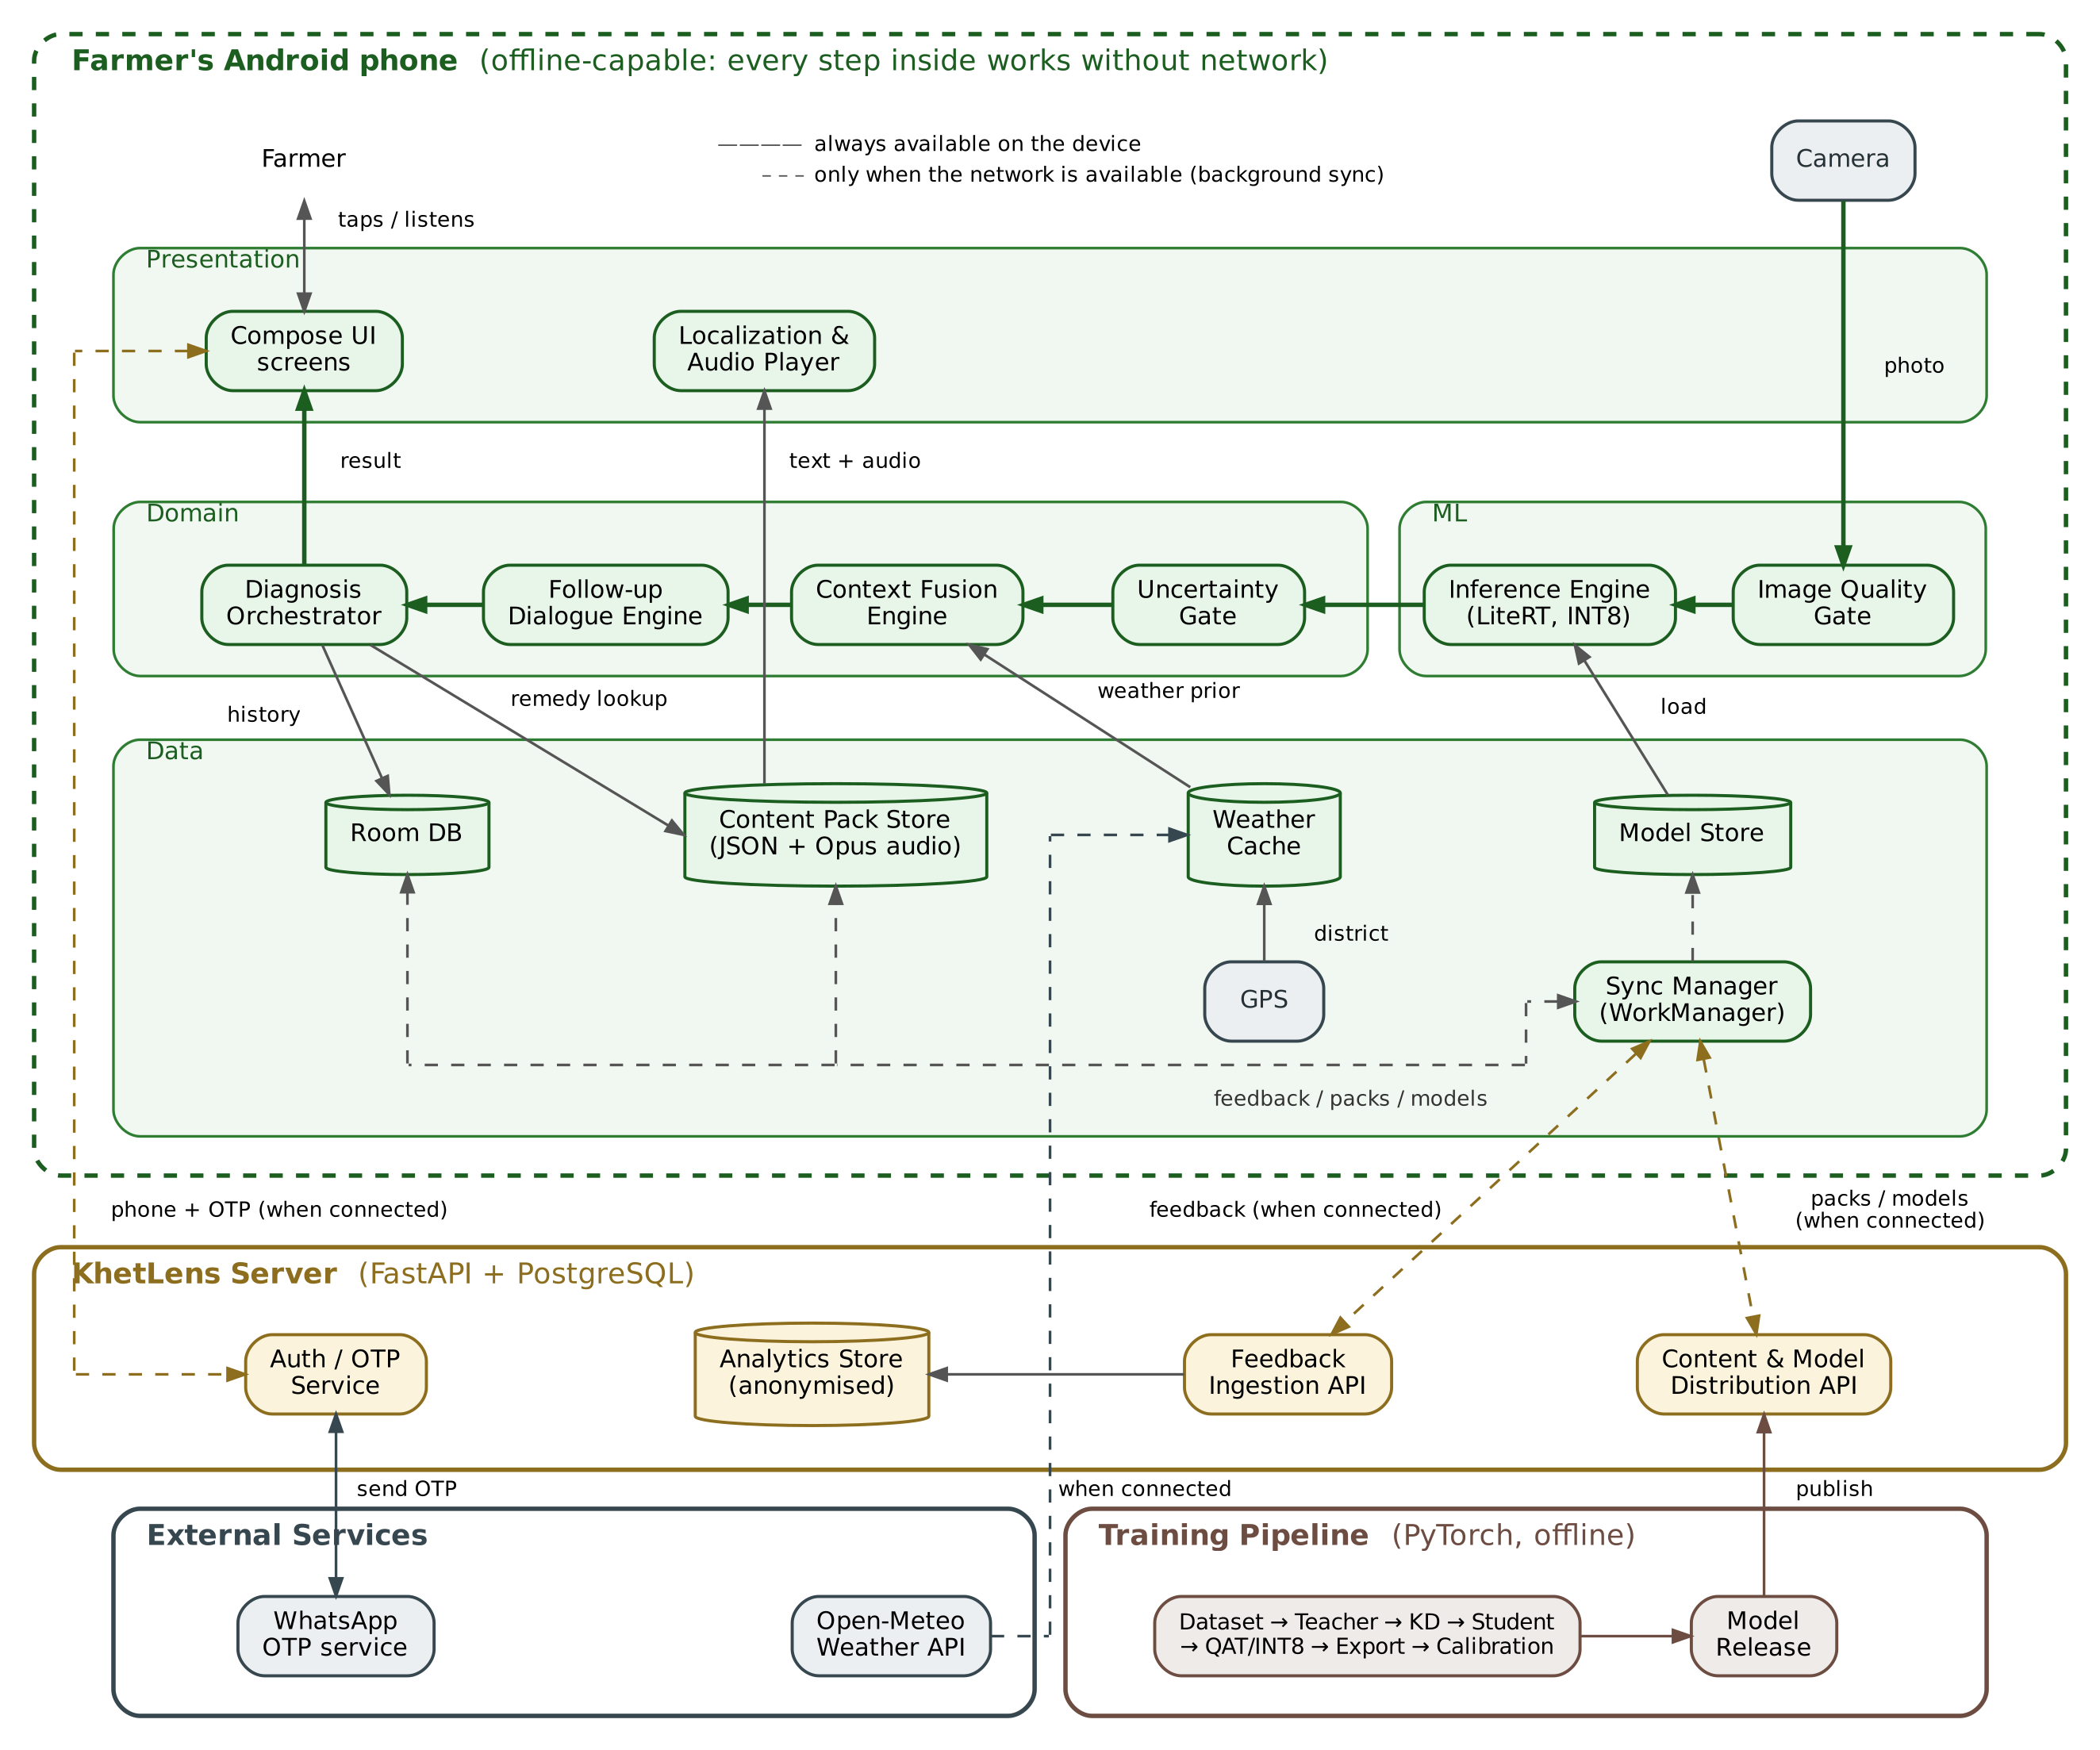
\includegraphics[width=\textwidth,height=0.88\textheight,keepaspectratio]{Figures/diagrams/architecture.png}
  \caption{High-level architecture of KhetLens. The mobile application (top) is fully functional offline; the server (middle) handles verification, feedback, distribution and analytics; the external services are the weather API and the WhatsApp code service; the offline training pipeline publishes model releases.}
  \label{fig:arch}
\end{figure}

The mobile application has four layers. The \emph{presentation} layer holds the screens, view models, localisation and audio player. The \emph{domain} layer holds the diagnostic logic independent of UI and storage: the diagnosis orchestrator (which runs Algorithm~\ref{algo:gate}), the weather adjustment and the follow-up engine. The \emph{ML} layer wraps the model: the image quality check, the inference engine and the uncertainty check. The \emph{data} layer holds persistence and I/O: the local database, the content pack store, the weather cache, the model store and the sync manager. Dependencies point inwards, so the diagnostic logic can be tested on a desktop against recorded inputs. We chose this decomposition because it separates the three things that change for different reasons: the interface (farmer feedback), the diagnostic logic (research results) and the platform code. A decomposition by feature was considered and set aside because the diagnostic core is shared by several features.

\subsection{Subsystem Architecture}
\textbf{Diagnosis subsystem.} Figure~\ref{fig:sub-diag} details the component every photograph passes through. The quality check computes the sharpness and exposure measures. The inference engine owns the interpreter, created once at start-up and reused; it runs the model on the whole photograph and, for wider shots, on its regions, and combines the outputs (Section~\ref{sec:multiscale}). The uncertainty check holds the release's statistics in memory. The weather adjustment reads the table from the content pack and the latest snapshot from the cache. The follow-up engine holds the question set and performs the update after each answer. The three outcomes are modelled as a sealed type so that every screen must handle every case.

\begin{figure}[H]
  \centering
  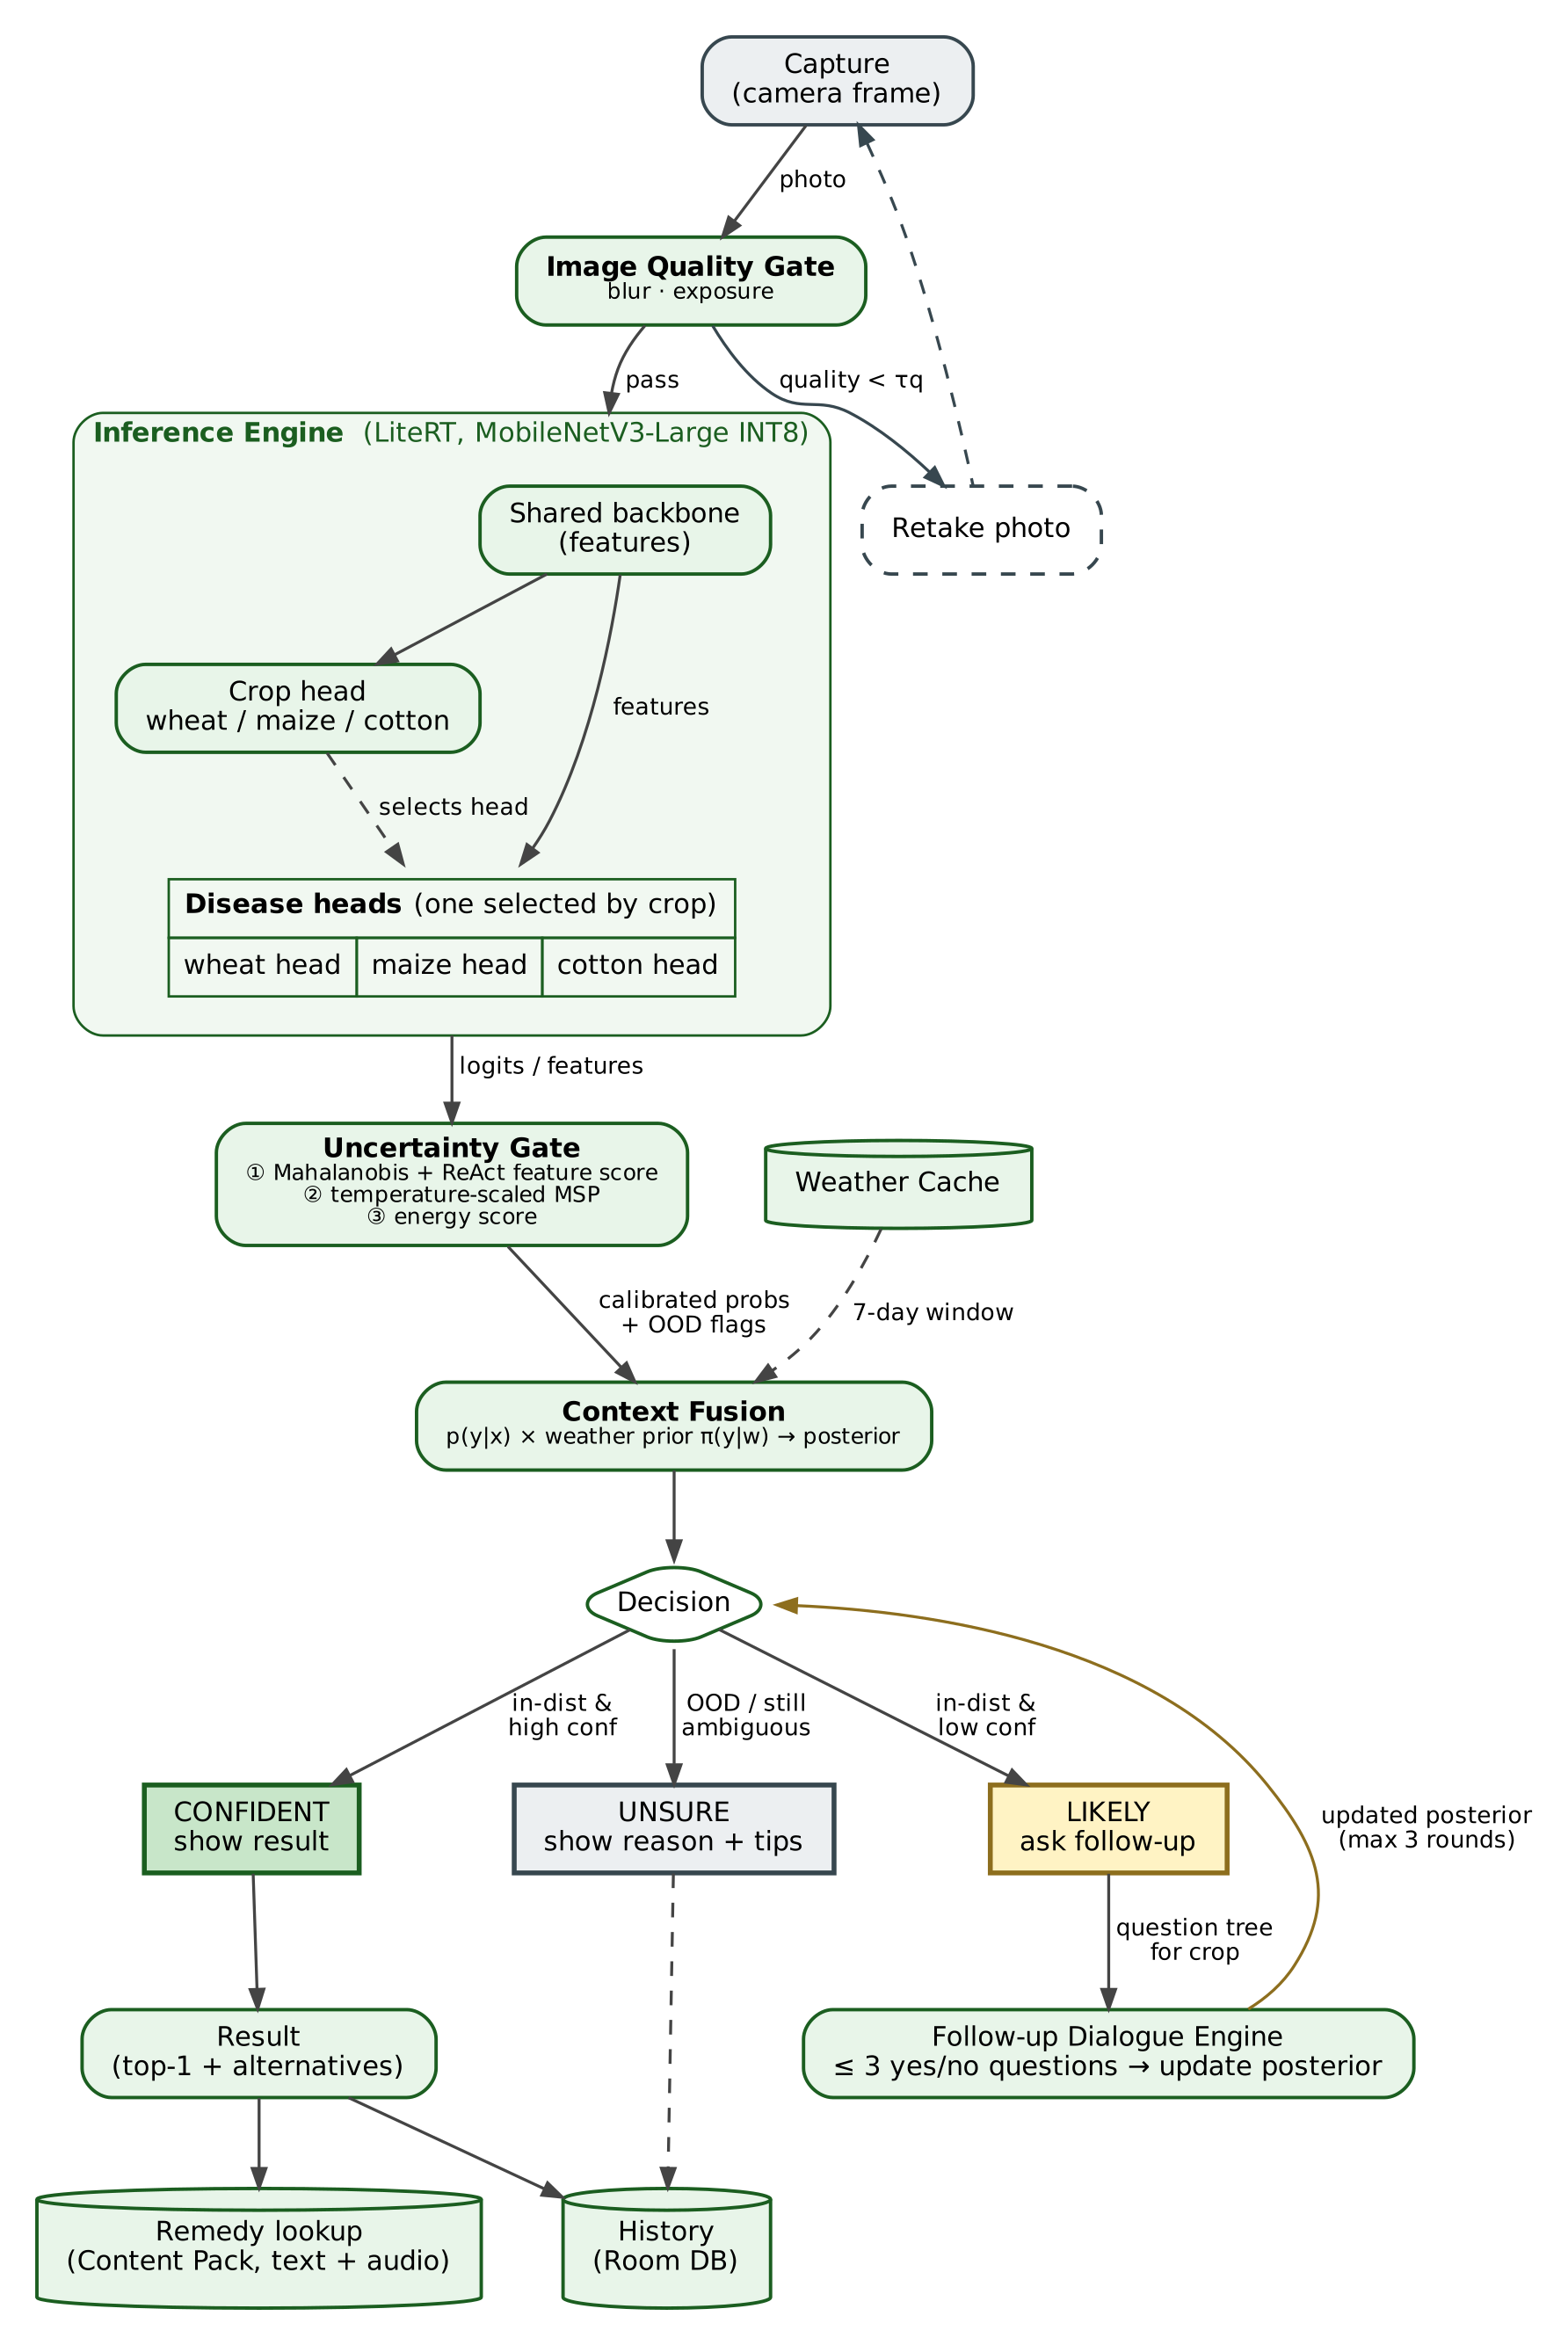
\includegraphics[width=\textwidth,height=0.88\textheight,keepaspectratio]{Figures/diagrams/subsystem_diagnosis.png}
  \caption{Component diagram of the diagnosis subsystem, from capture through the quality check, inference, uncertainty check and weather adjustment to the three outcomes, guidance lookup and history.}
  \label{fig:sub-diag}
\end{figure}

\textbf{Backend subsystem.} Figure~\ref{fig:sub-backend} shows the server. The FastAPI application has four routers. \emph{Auth} requests and verifies one-time codes through the WhatsApp service, limits requests per number, and returns a signed token; it stores only a hash of the number. \emph{Feedback} accepts batches of feedback records, deduplicates them by client-generated identifier so that retries are safe, and writes them to the database; opted-in images go to object storage. \emph{Distribution} serves version information and download links for content packs and model releases. \emph{Analytics} serves aggregate counts per district, crop and condition to the team. Our publish tool validates and uploads packs and releases after agronomist review.

\begin{figure}[H]
  \centering
  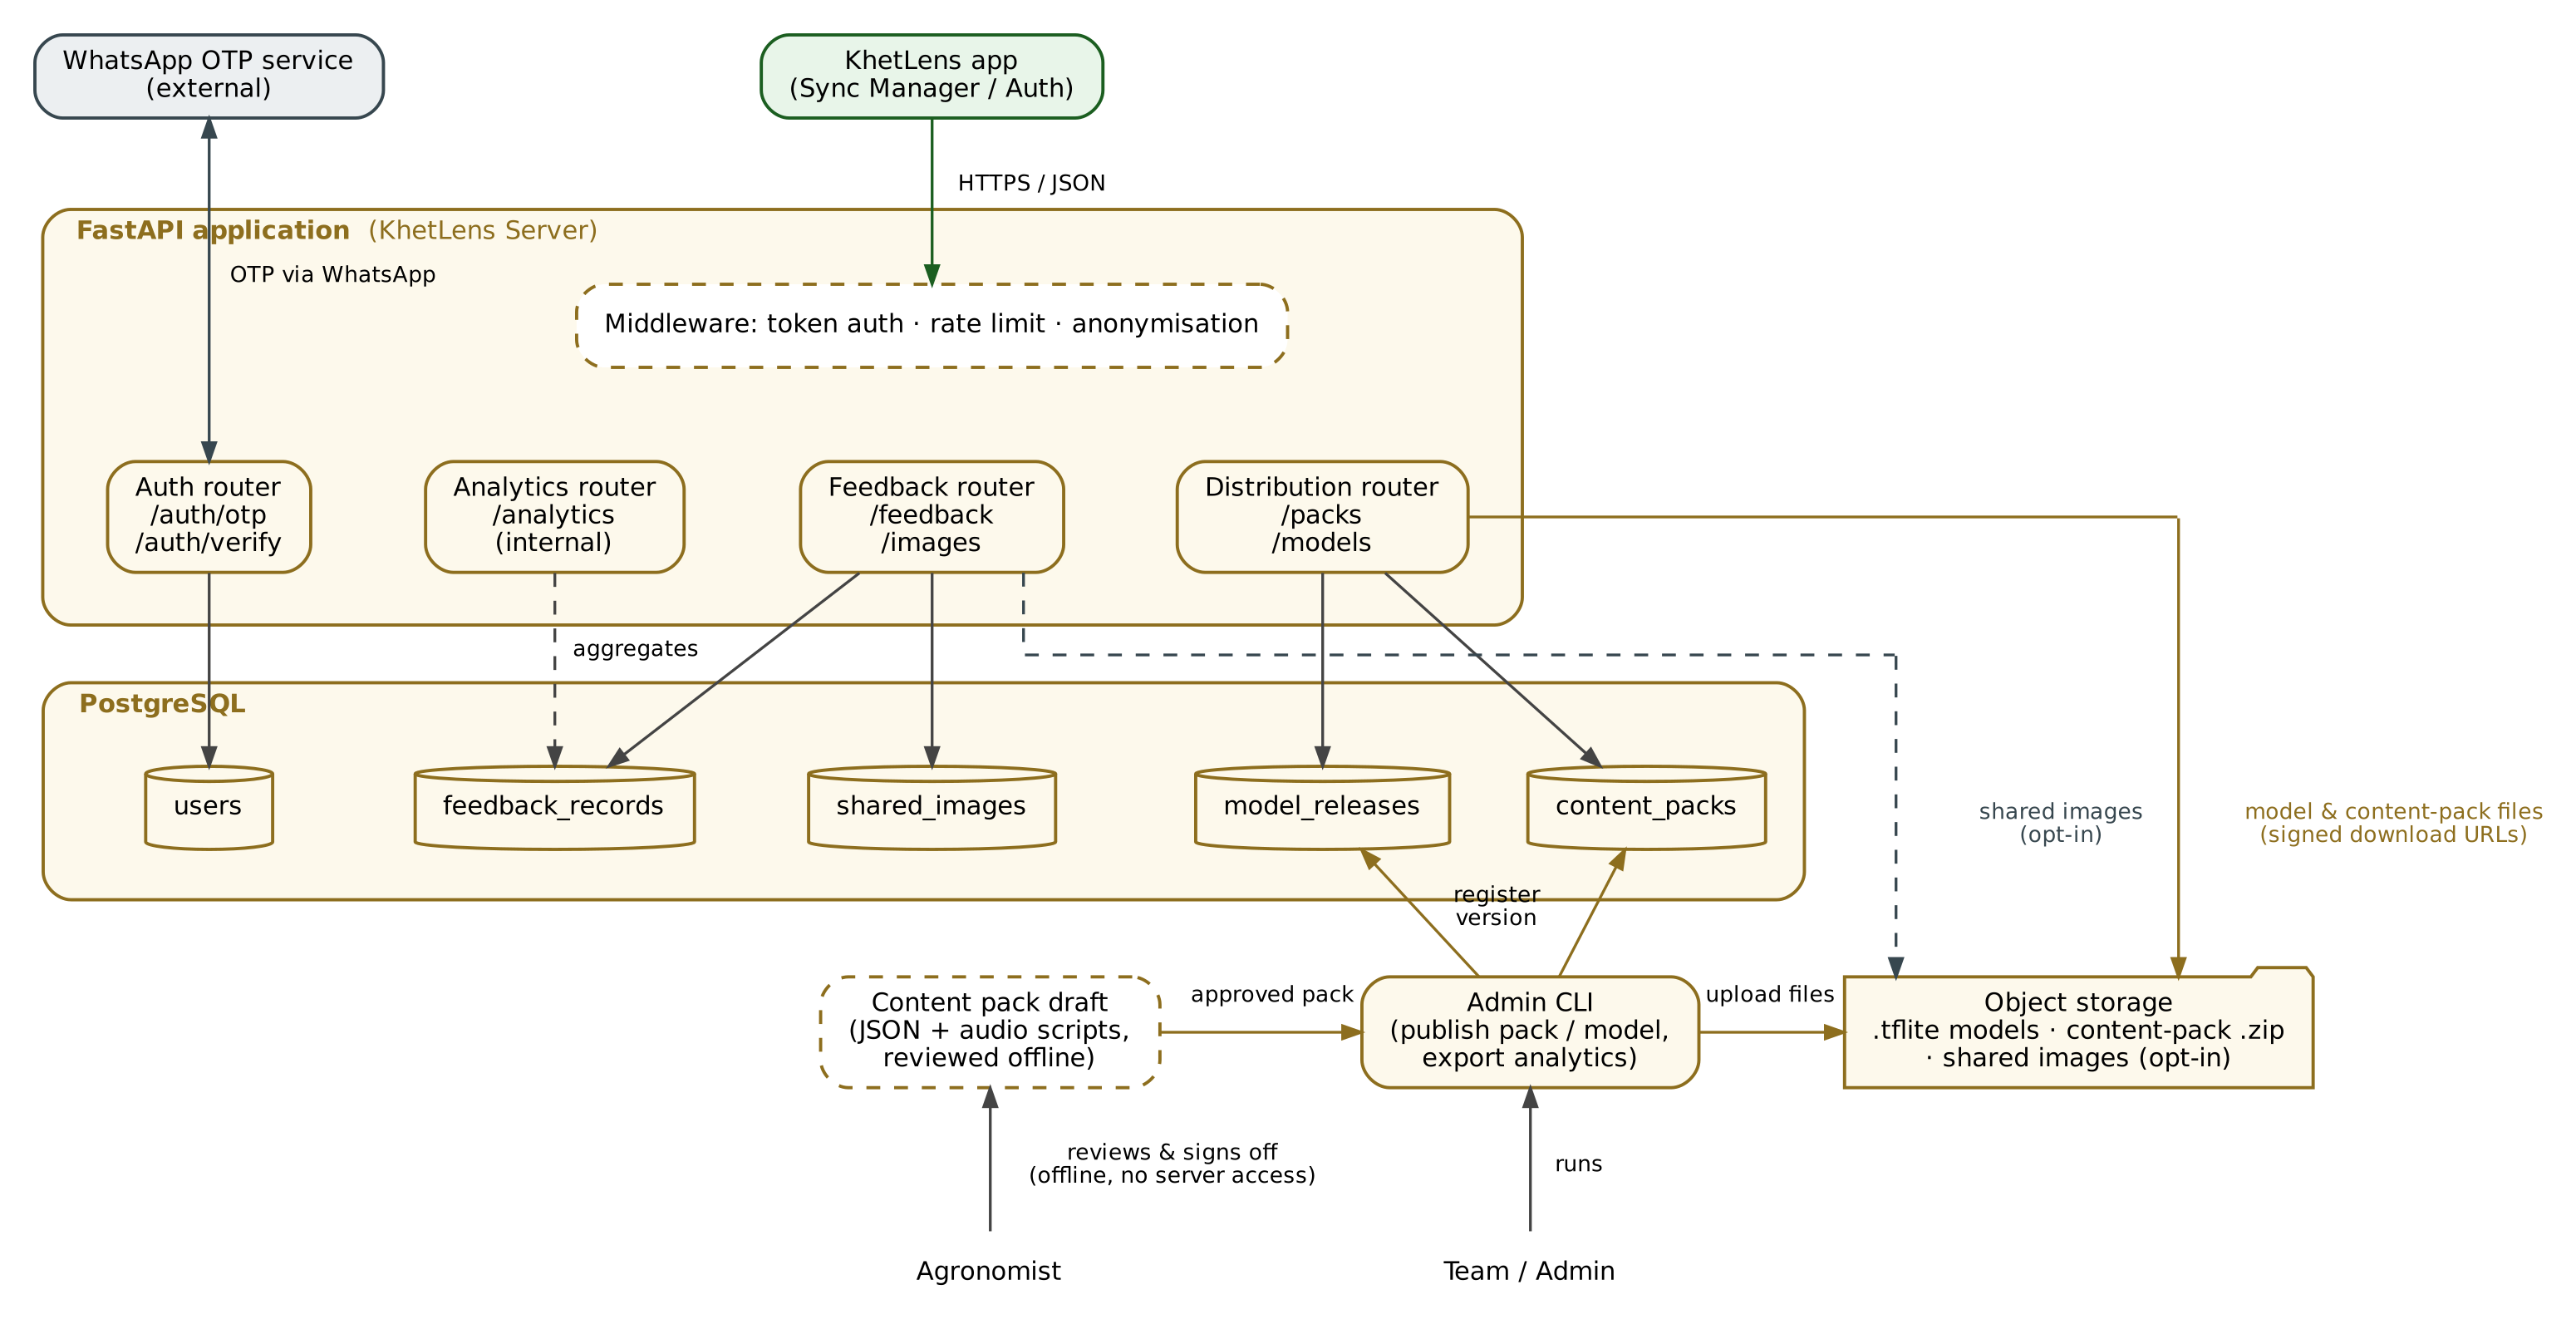
\includegraphics[width=\textwidth,height=0.88\textheight,keepaspectratio]{Figures/diagrams/subsystem_backend.png}
  \caption{Component diagram of the KhetLens server: routers, database tables, object storage, our publish tool and the agronomist review that precedes publication.}
  \label{fig:sub-backend}
\end{figure}

\section{Architectural Strategies}
Each strategy records the decision, the alternatives considered and the reasons.

\subsection{Local-compute, offline-first inference}
\textbf{Decision:} the full diagnosis runs on the device; there is no cloud inference path. \textbf{Alternatives:} cloud inference, or a hybrid with cloud fallback. \textbf{Reasons:} connectivity is the defining constraint of the problem; compact models have been run on entry-level phones in the field~\cite{ramcharan2019cassava} and quantised MobileNetV3 models are small and fast~\cite{khan2023edge}; privacy follows by construction; a single code path is easier to test.

\subsection{Native Android application}
\textbf{Decision:} Kotlin with Jetpack Compose. \textbf{Alternatives:} Flutter, React Native. \textbf{Reasons:} first-class support for the inference runtime, camera and local database; small install size; reliable right-to-left and Nastaliq rendering; Android-only scope.

\subsection{Quantised model with a measured runtime choice}
\textbf{Decision:} 8-bit integer model on TensorFlow Lite, with ONNX Runtime benchmarked as an alternative. \textbf{Alternatives:} 16-bit floats; other mobile runtimes. \textbf{Reasons:} integer models are smaller and faster on CPUs, and runtime choice has a large effect on latency~\cite{zhangq2022mobilebench}, so we measure rather than assume.

\subsection{Shared backbone with crop and per-crop disease heads}
\textbf{Decision:} one network with a crop head and three disease heads. \textbf{Alternatives:} three separate models, or one flat 17-way classifier. \textbf{Reasons:} crop-conditional design improved field accuracy in prior work~\cite{picon2019cropcond}; classes can be added to one head without retraining the backbone; the crop head gives a natural confirmation step.

\subsection{Rule-based weather adjustment}
\textbf{Decision:} multiply calibrated probabilities by a prior from a reviewed table (Equation~\ref{eq:fusion}). \textbf{Alternatives:} learned fusion of weather features inside the network. \textbf{Reasons:} transparency to agronomists and farmers (the Why panel can state the weather cue), no need for paired training data, editability without retraining, and graceful fallback when weather is unavailable.

\subsection{Data as content in versioned packs}
\textbf{Decision:} disease entries, guidance, questions, the weather table and audio form a validated, versioned content pack downloaded and swapped atomically. \textbf{Alternatives:} content compiled into the app; a server-rendered content API. \textbf{Reasons:} agronomist corrections should not need an app release; the pack is also the unit of review and attribution.

\subsection{Opportunistic, retry-safe synchronisation}
\textbf{Decision:} all network work runs in deferred background jobs with network constraints, back-off and client-generated identifiers. \textbf{Alternatives:} synchronous calls at the moment of action. \textbf{Reasons:} the farmer is never blocked, and retries cannot create duplicates.

\subsection{Privacy by default}
\textbf{Decision:} photographs and GPS coordinates stay on the device; the server receives district, crop, outcome, confidence and versions; sharing a photograph is a per-feedback opt-in. \textbf{Reasons:} NFR-08 and the trust that farmer adoption depends on~\cite{soodan2024adoption}.

\subsection{Error detection and recovery}
Every external interaction has a defined failure behaviour: a failed quality check returns to the viewfinder with a reason; a model that fails to load falls back to the last working one, ultimately the baseline bundled in the app (FR-26); a corrupt or partial download is discarded; stale weather yields a uniform prior and a visible note; a failed sign-in offers retry and guest mode; database writes are transactional so an interrupted diagnosis leaves no partial record.

\subsection{Concurrency and memory}
Inference runs on a dedicated single-threaded dispatcher so that two diagnoses never contend for the interpreter; live preview analysis runs on a separate dispatcher with frame dropping. Images are decoded at the model's input size directly from the camera buffer; history photographs are stored downscaled and removed with their records after six months.

\section{Domain Model/Class Diagram}
Figure~\ref{fig:class} shows the domain model of the mobile application. The persistent entities map onto the tables of Section~\ref{sec:db}: \texttt{User}, \texttt{Diagnosis}, \texttt{WeatherSnapshot}, \texttt{Remedy} and \texttt{Feedback} to the tables of the same name, \texttt{Disease} to \texttt{condition}, and \texttt{ContentPack} to \texttt{content\_pack\_version}; \texttt{ModelRelease} is the manifest of the installed model. The services carry behaviour: \texttt{DiagnosisOrchestrator} implements Algorithm~\ref{algo:gate} by composing \texttt{InferenceEngine}, \texttt{UncertaintyGate}, \texttt{ContextFusionEngine} and \texttt{FollowUpEngine}; \texttt{WeatherRepository} and \texttt{ContentRepository} are interfaces implemented in the data layer; \texttt{SyncManager} schedules the background jobs.

\begin{figure}[H]
  \centering
  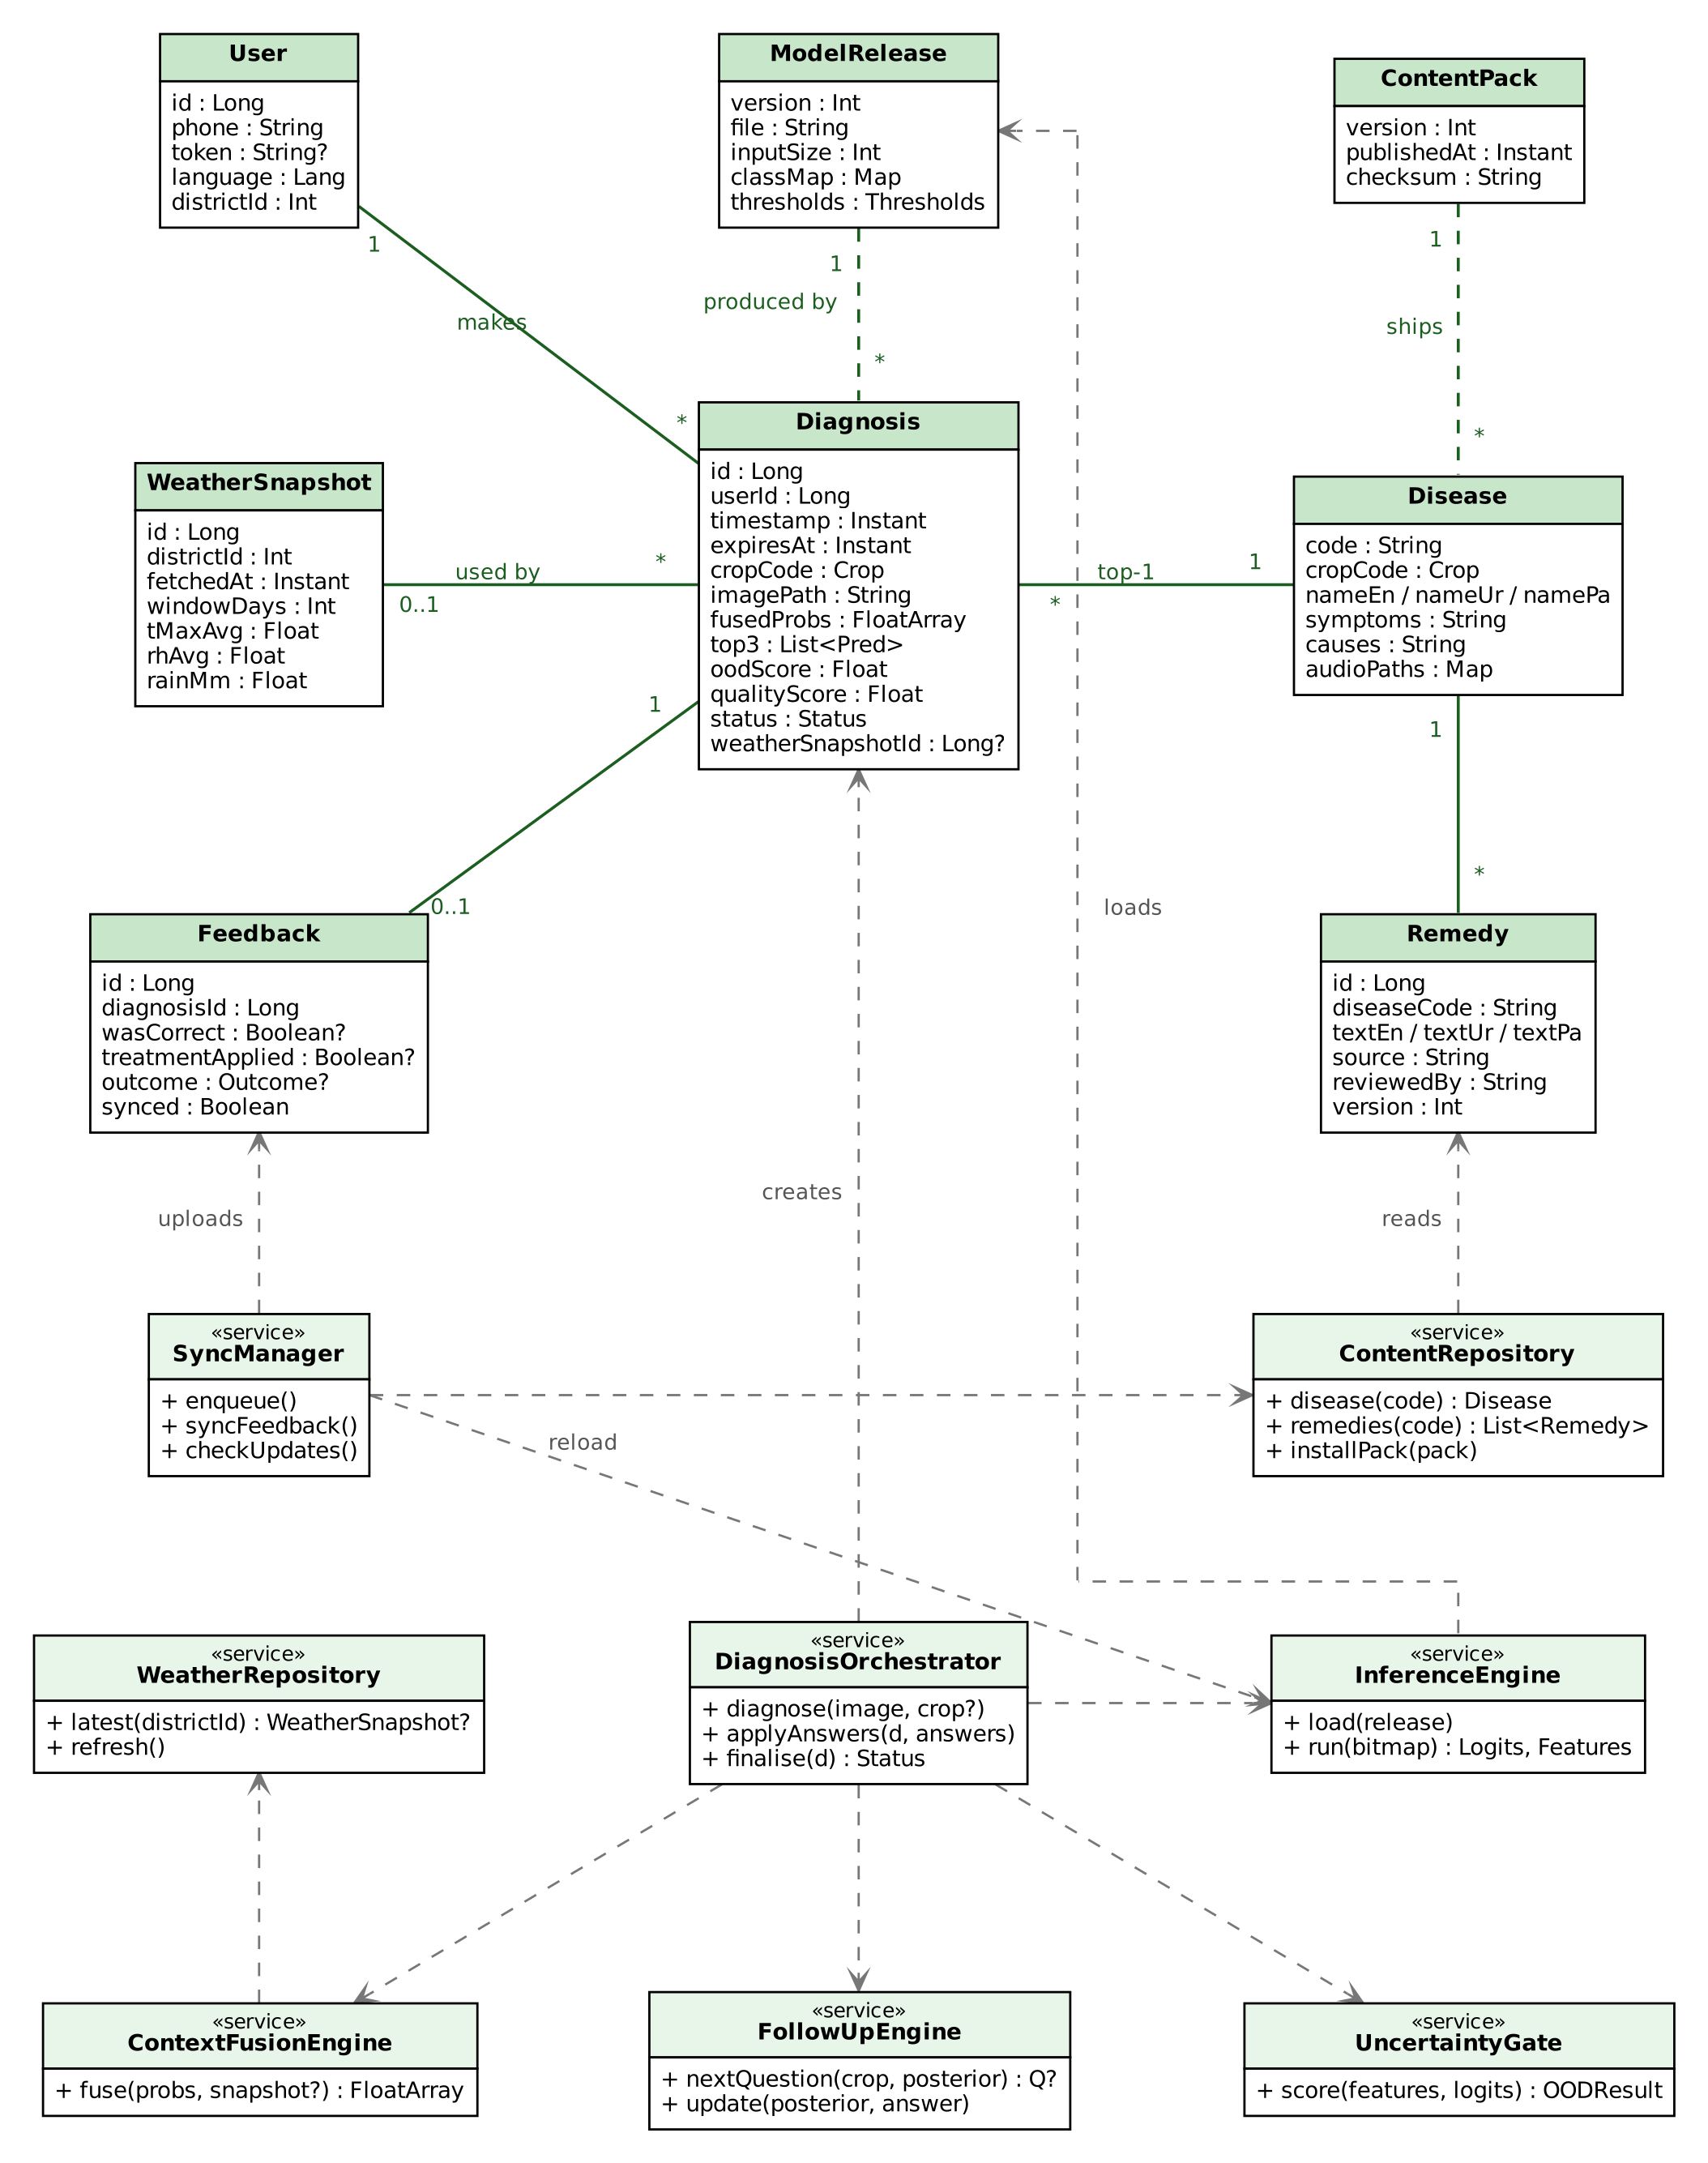
\includegraphics[width=\textwidth,height=0.88\textheight,keepaspectratio]{Figures/diagrams/class_diagram.png}
  \caption{Class diagram of the mobile application: persistent entities with their key attributes and relationships, and the domain and data services that operate on them.}
  \label{fig:class}
\end{figure}

\section{Sequence Diagrams}
Five interactions define the system's behaviour; each is traced to its use case.

\textbf{Diagnose a plant (UC-04, UC-05).} Figure~\ref{fig:seq-diag} shows the main path and the quality-check rejection. The shutter tap hands the frame to the diagnosis engine, which checks quality, runs the model, applies the uncertainty check and the weather adjustment, stores the record and returns the outcome to the screen.

\begin{figure}[H]
  \centering
  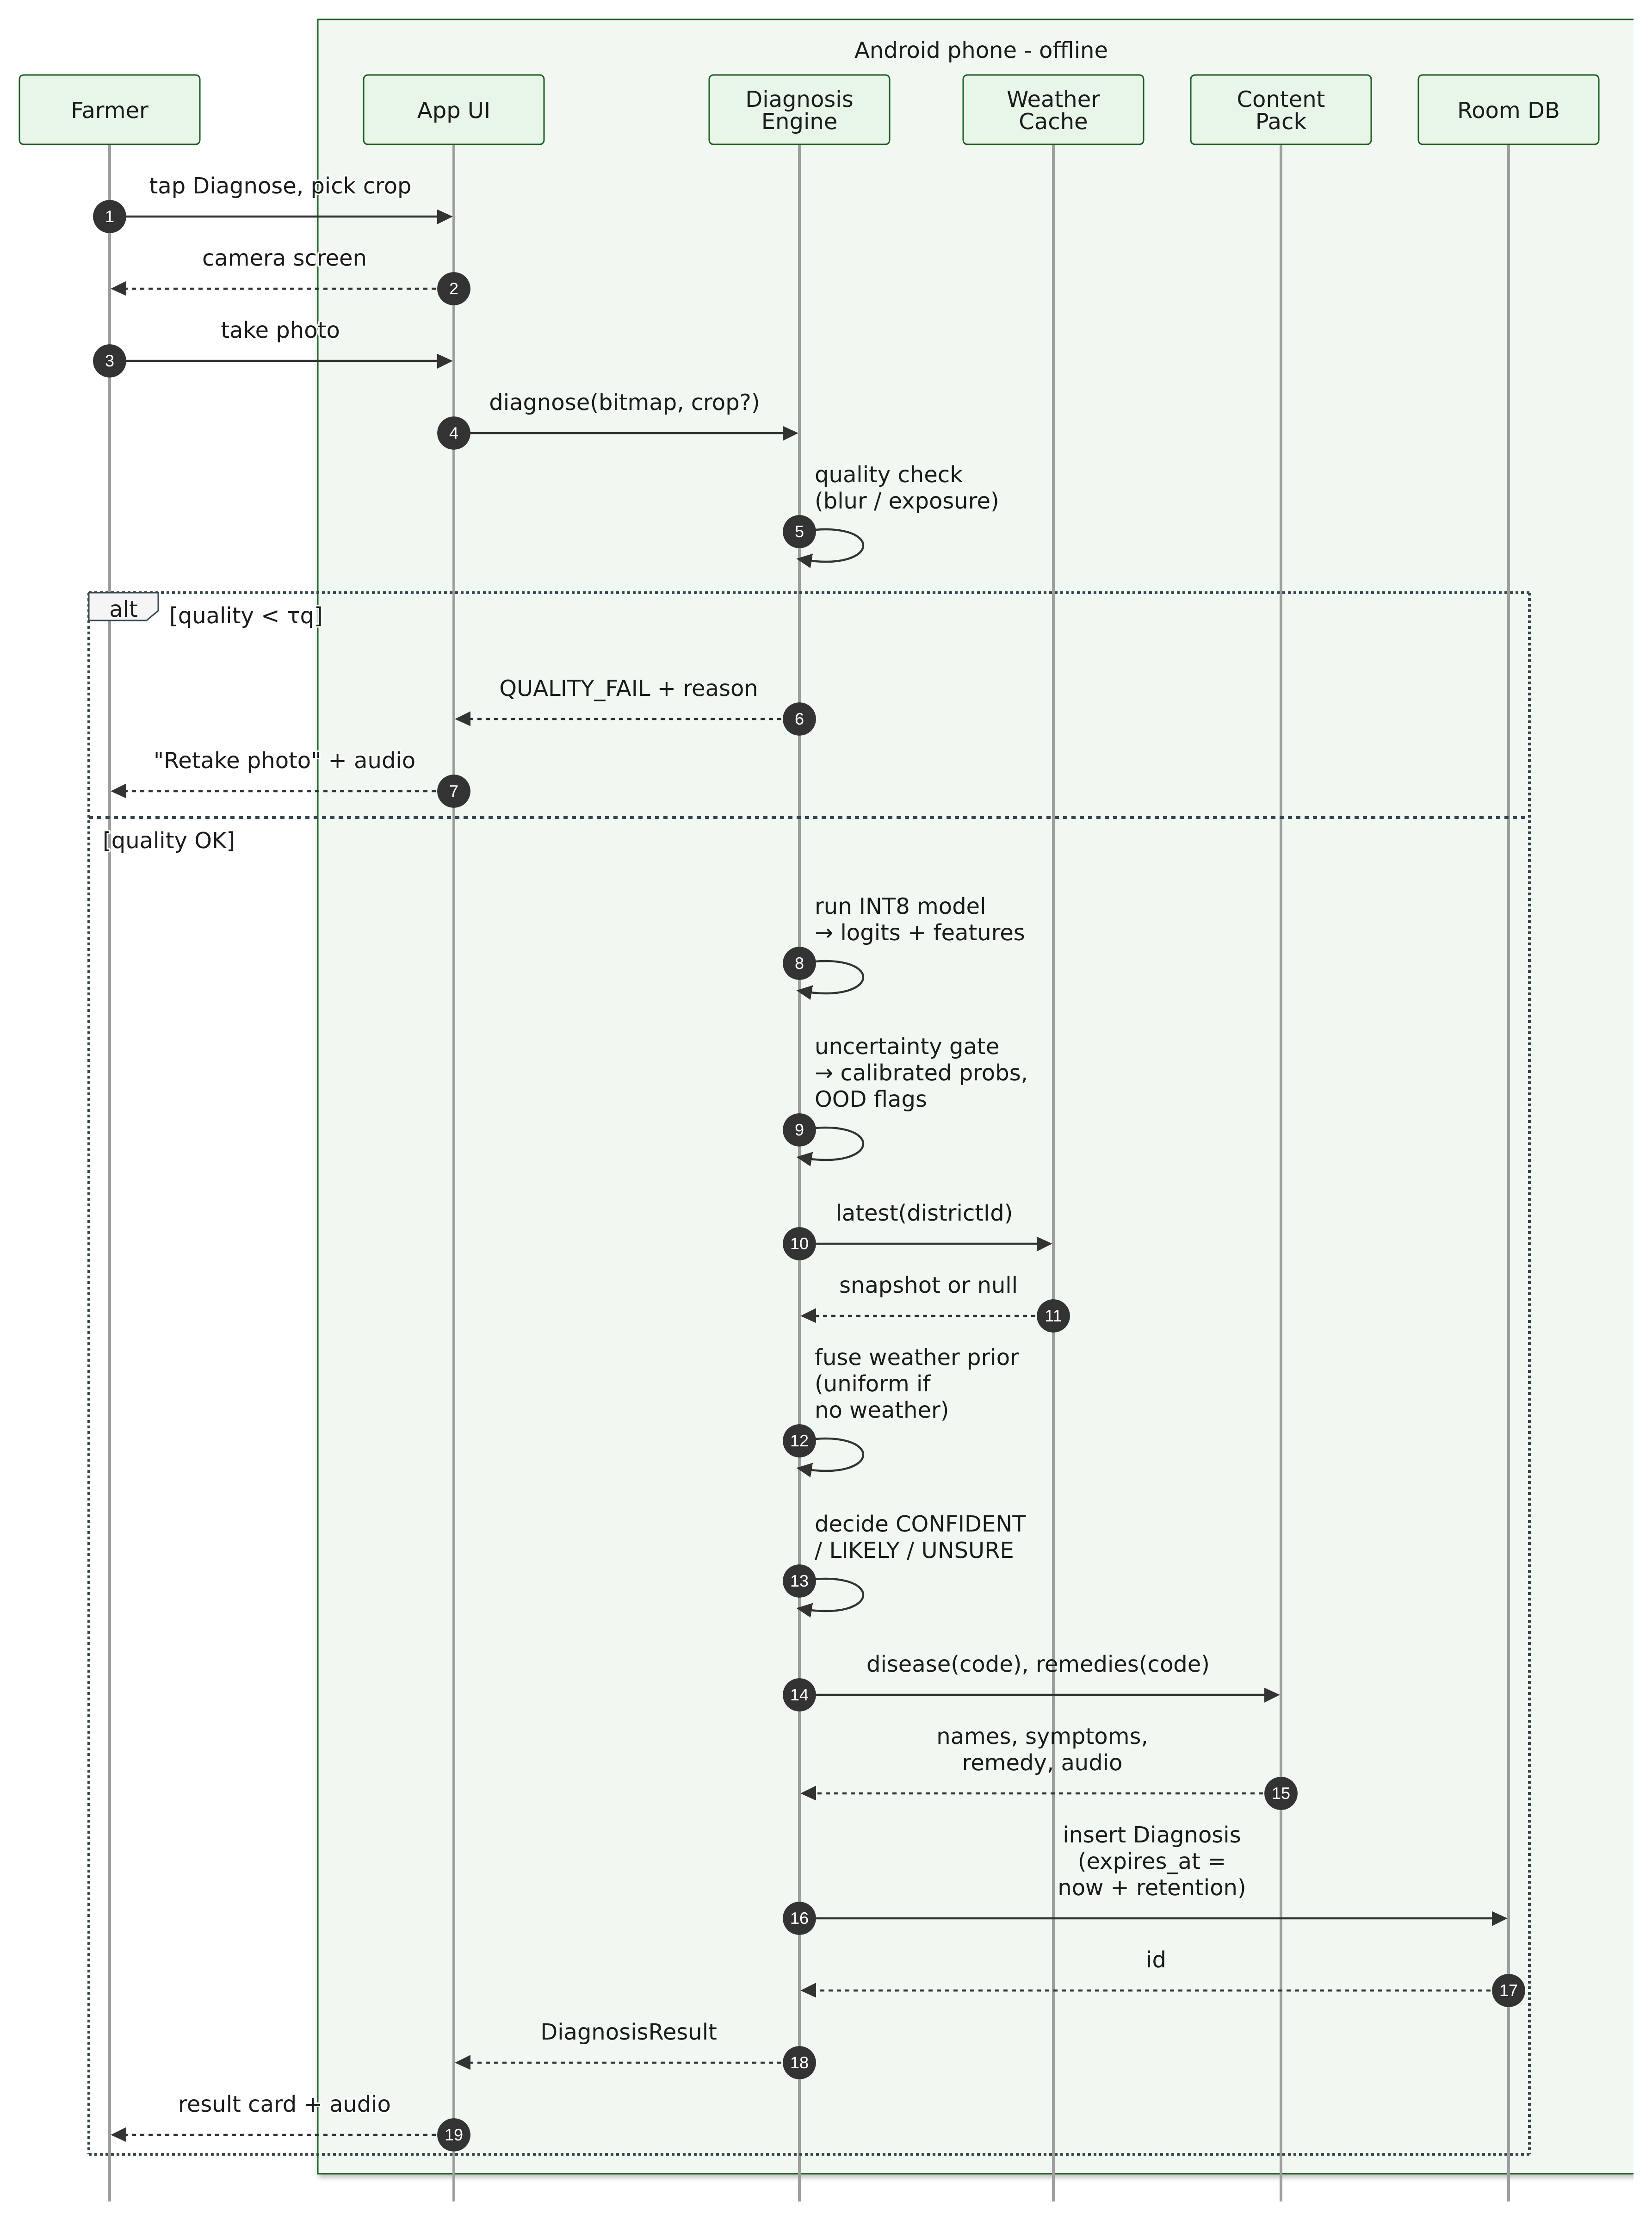
\includegraphics[width=\textwidth,height=0.88\textheight,keepaspectratio]{Figures/diagrams/seq_diagnose.png}
  \caption{Sequence diagram for a diagnosis, including the alternative flow in which the quality check rejects the photograph.}
  \label{fig:seq-diag}
\end{figure}

\textbf{Follow-up questions (UC-07).} Figure~\ref{fig:seq-follow} shows the Likely branch: the follow-up engine loads the crop's question set, the screen asks up to three questions, each answer updates the result, and the orchestrator finalises and stores the answers.

\begin{figure}[H]
  \centering
  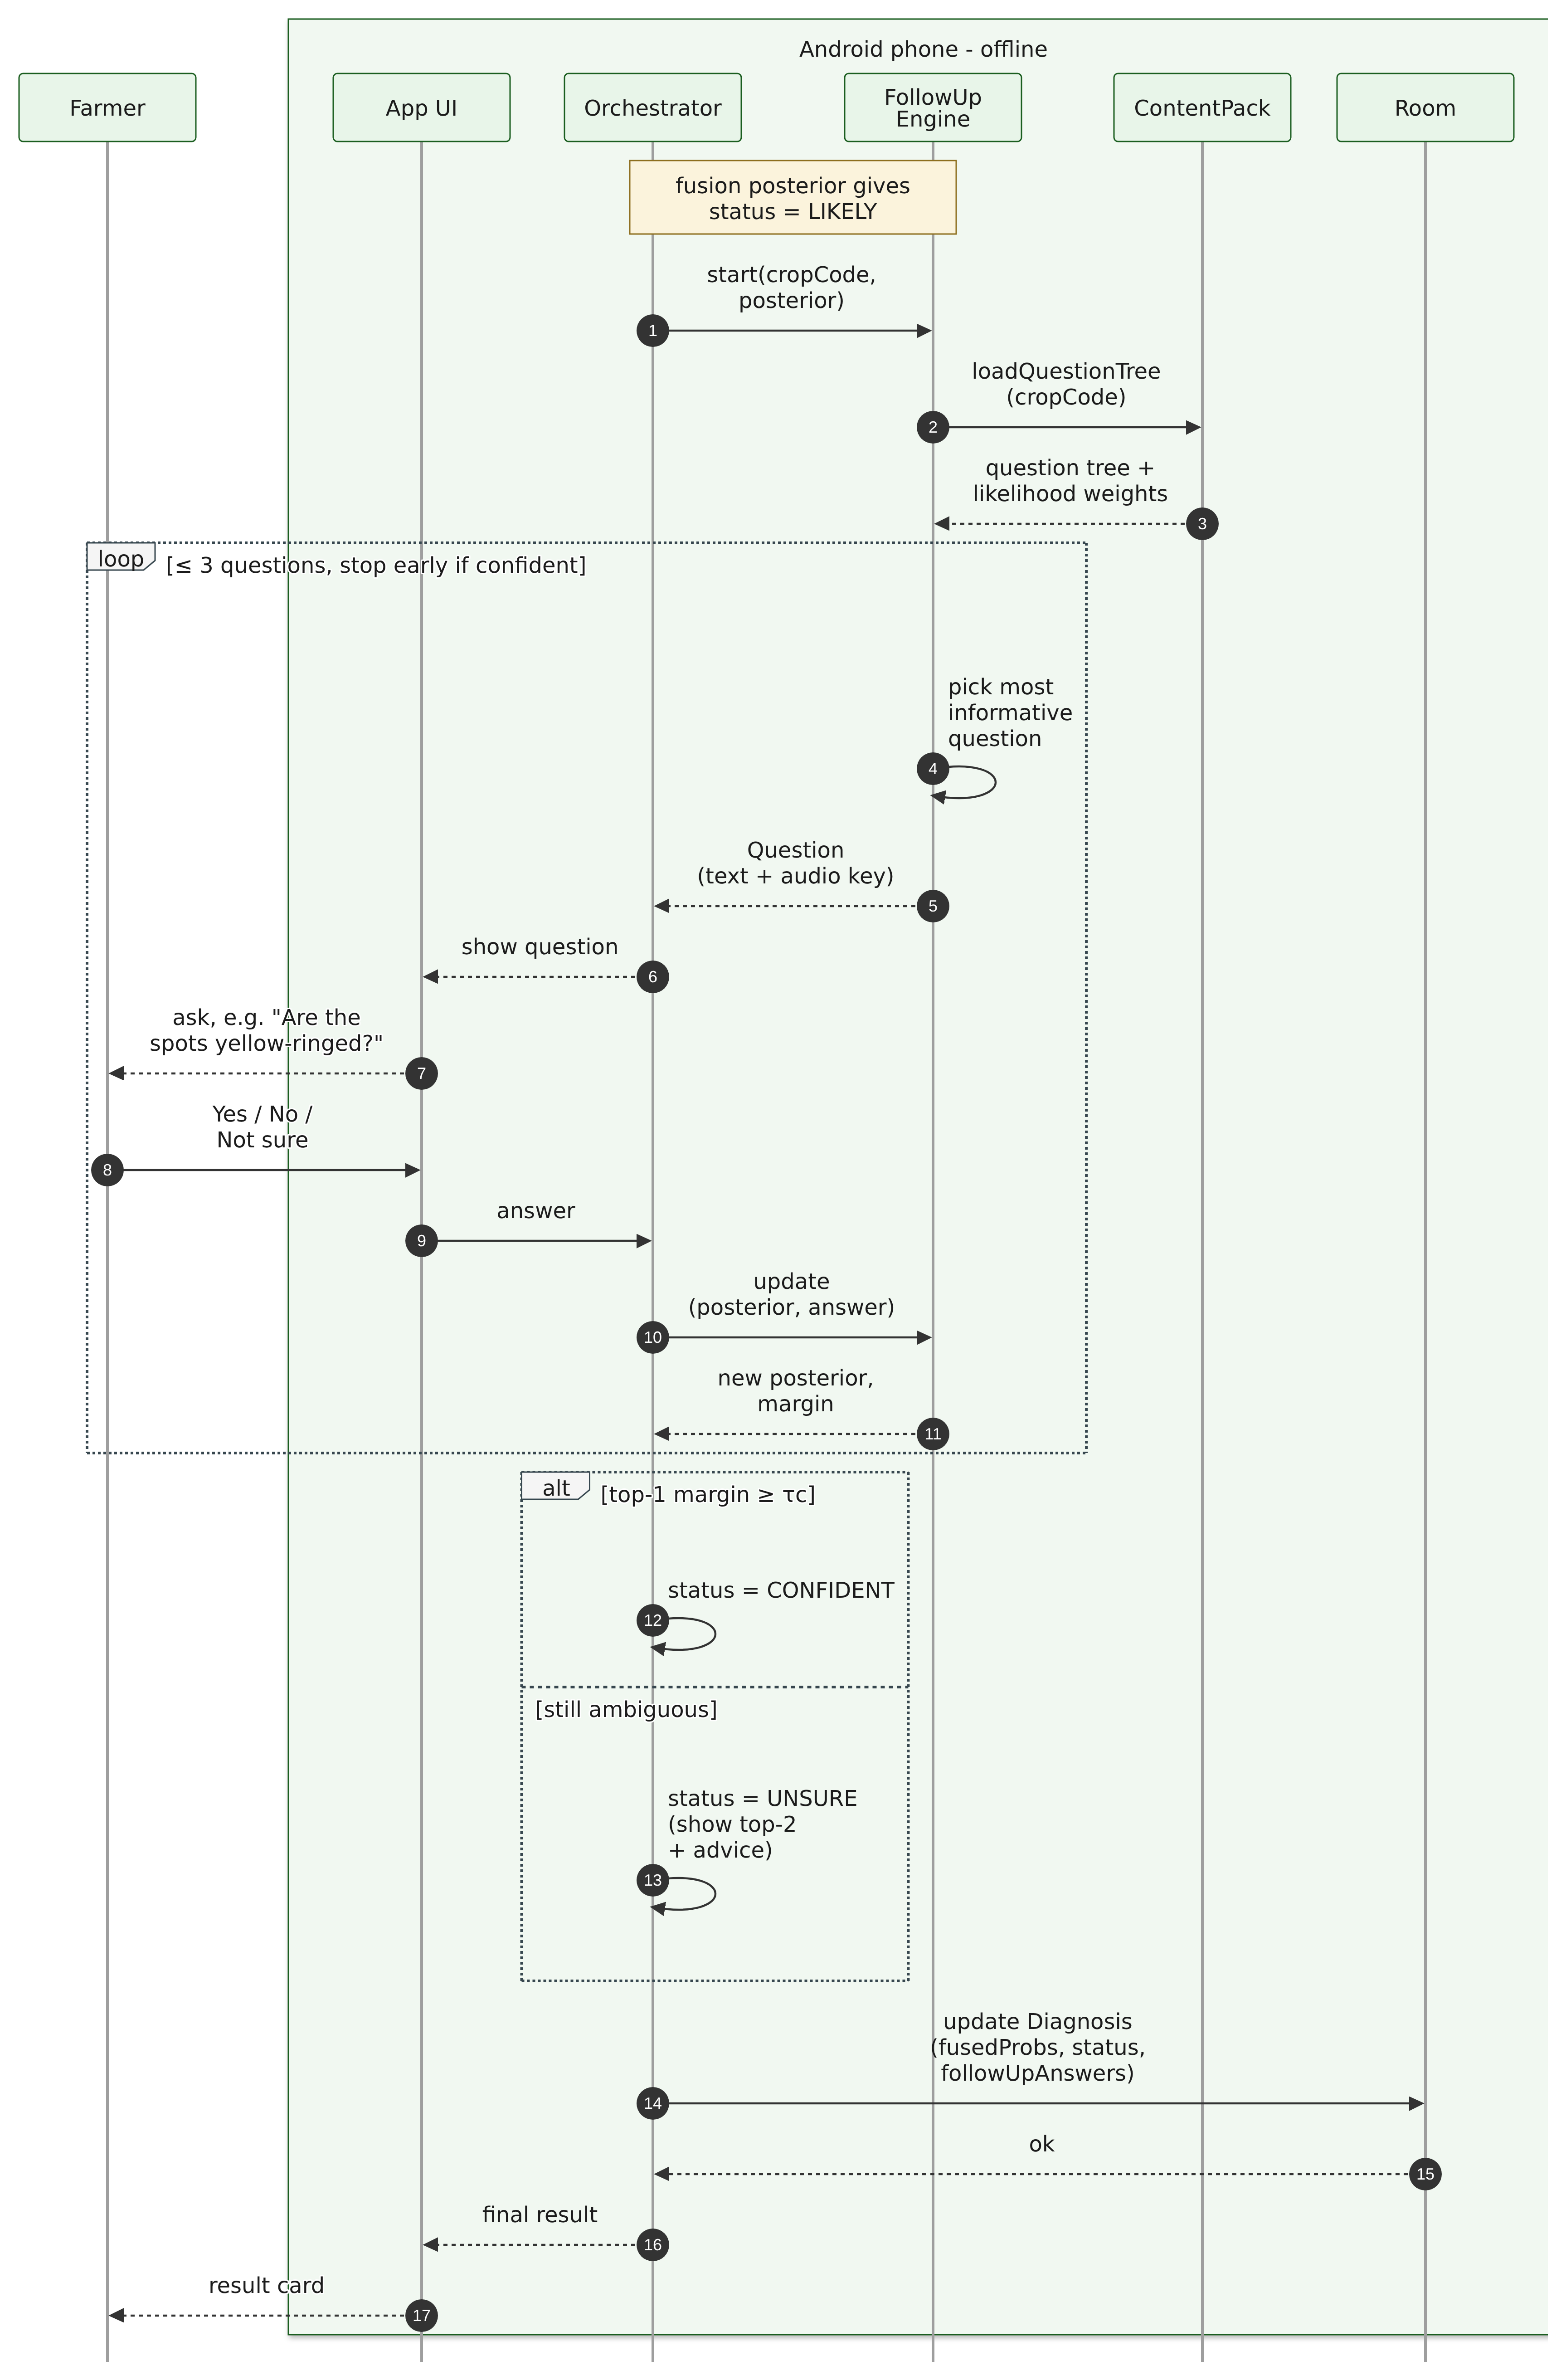
\includegraphics[width=\textwidth,height=0.88\textheight,keepaspectratio]{Figures/diagrams/seq_followup.png}
  \caption{Sequence diagram for the follow-up questions after a Likely outcome.}
  \label{fig:seq-follow}
\end{figure}

\textbf{Feedback synchronisation (UC-12, FR-24).} Figure~\ref{fig:seq-sync} shows feedback written locally as unsent, the background job that uploads it when connected, and the acknowledgement after which the local copy is deleted; offline, it simply stays queued.

\begin{figure}[H]
  \centering
  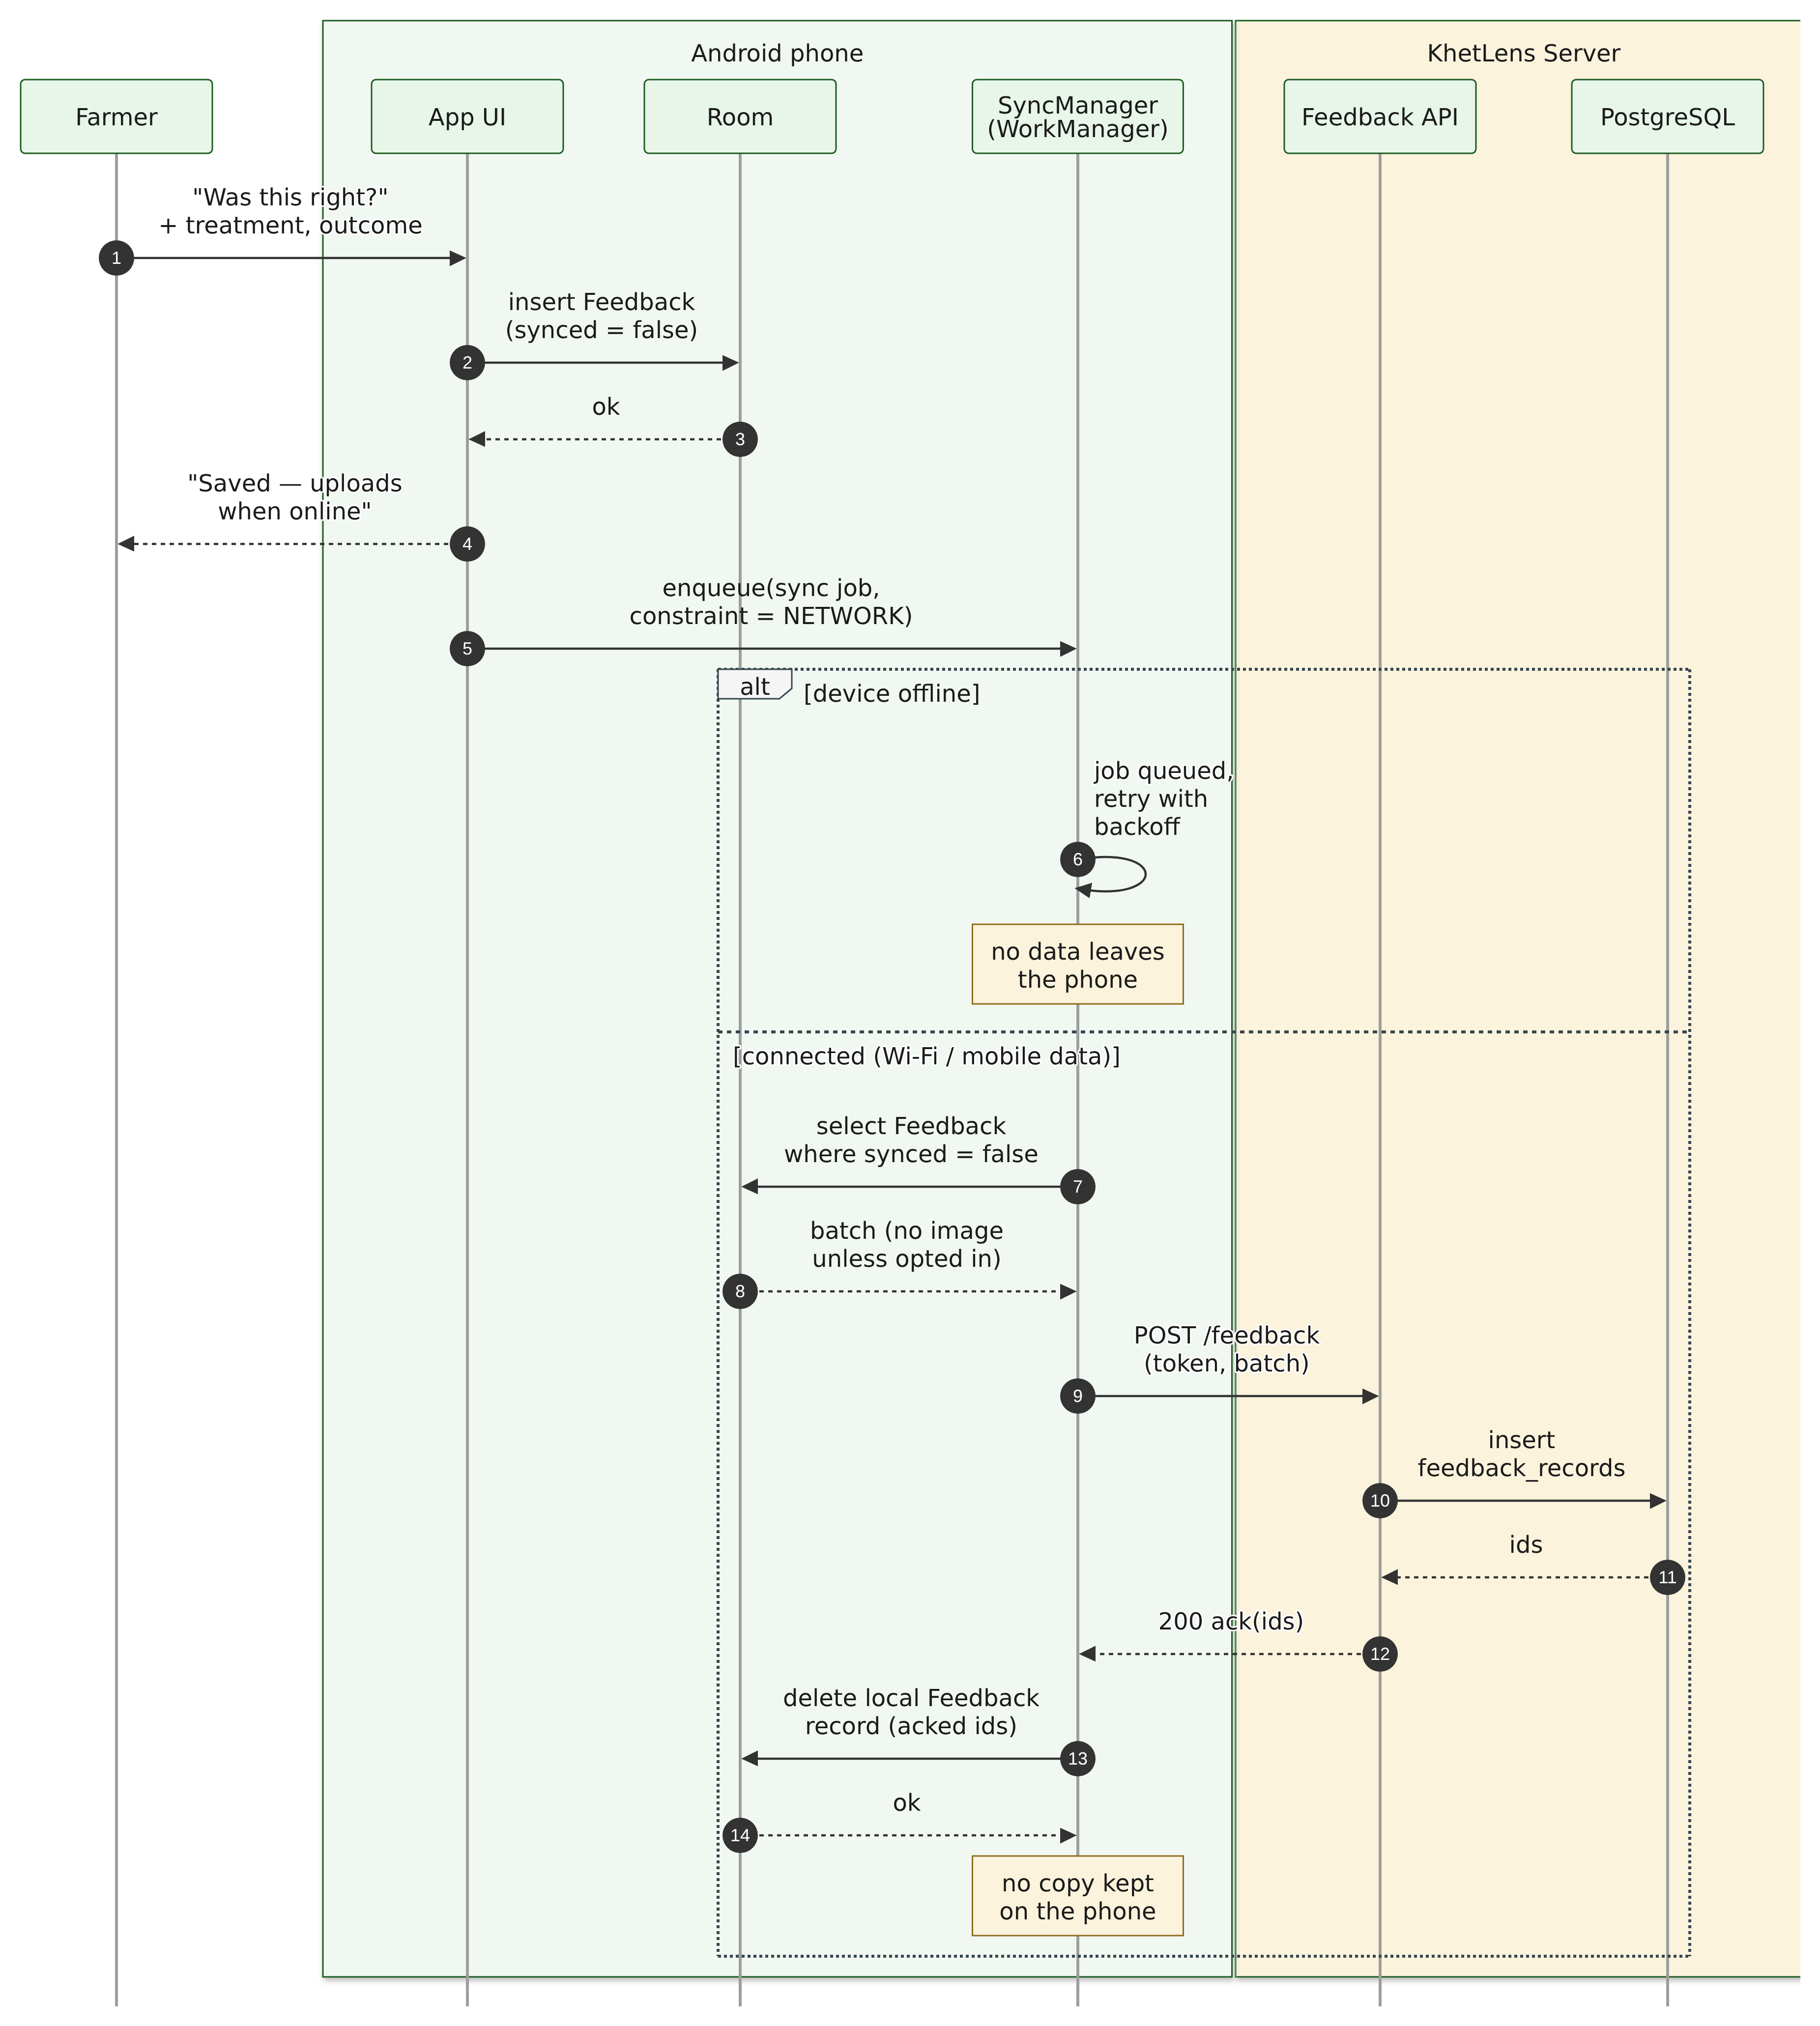
\includegraphics[width=\textwidth,height=0.88\textheight,keepaspectratio]{Figures/diagrams/seq_feedback_sync.png}
  \caption{Sequence diagram for offline feedback capture and later synchronisation.}
  \label{fig:seq-sync}
\end{figure}

\textbf{Sign-in (UC-02, UC-03).} Figure~\ref{fig:seq-login} shows the code request and verification through the server and the WhatsApp service, token storage, and the ``Skip for now'' alternative that creates a guest profile.

\begin{figure}[H]
  \centering
  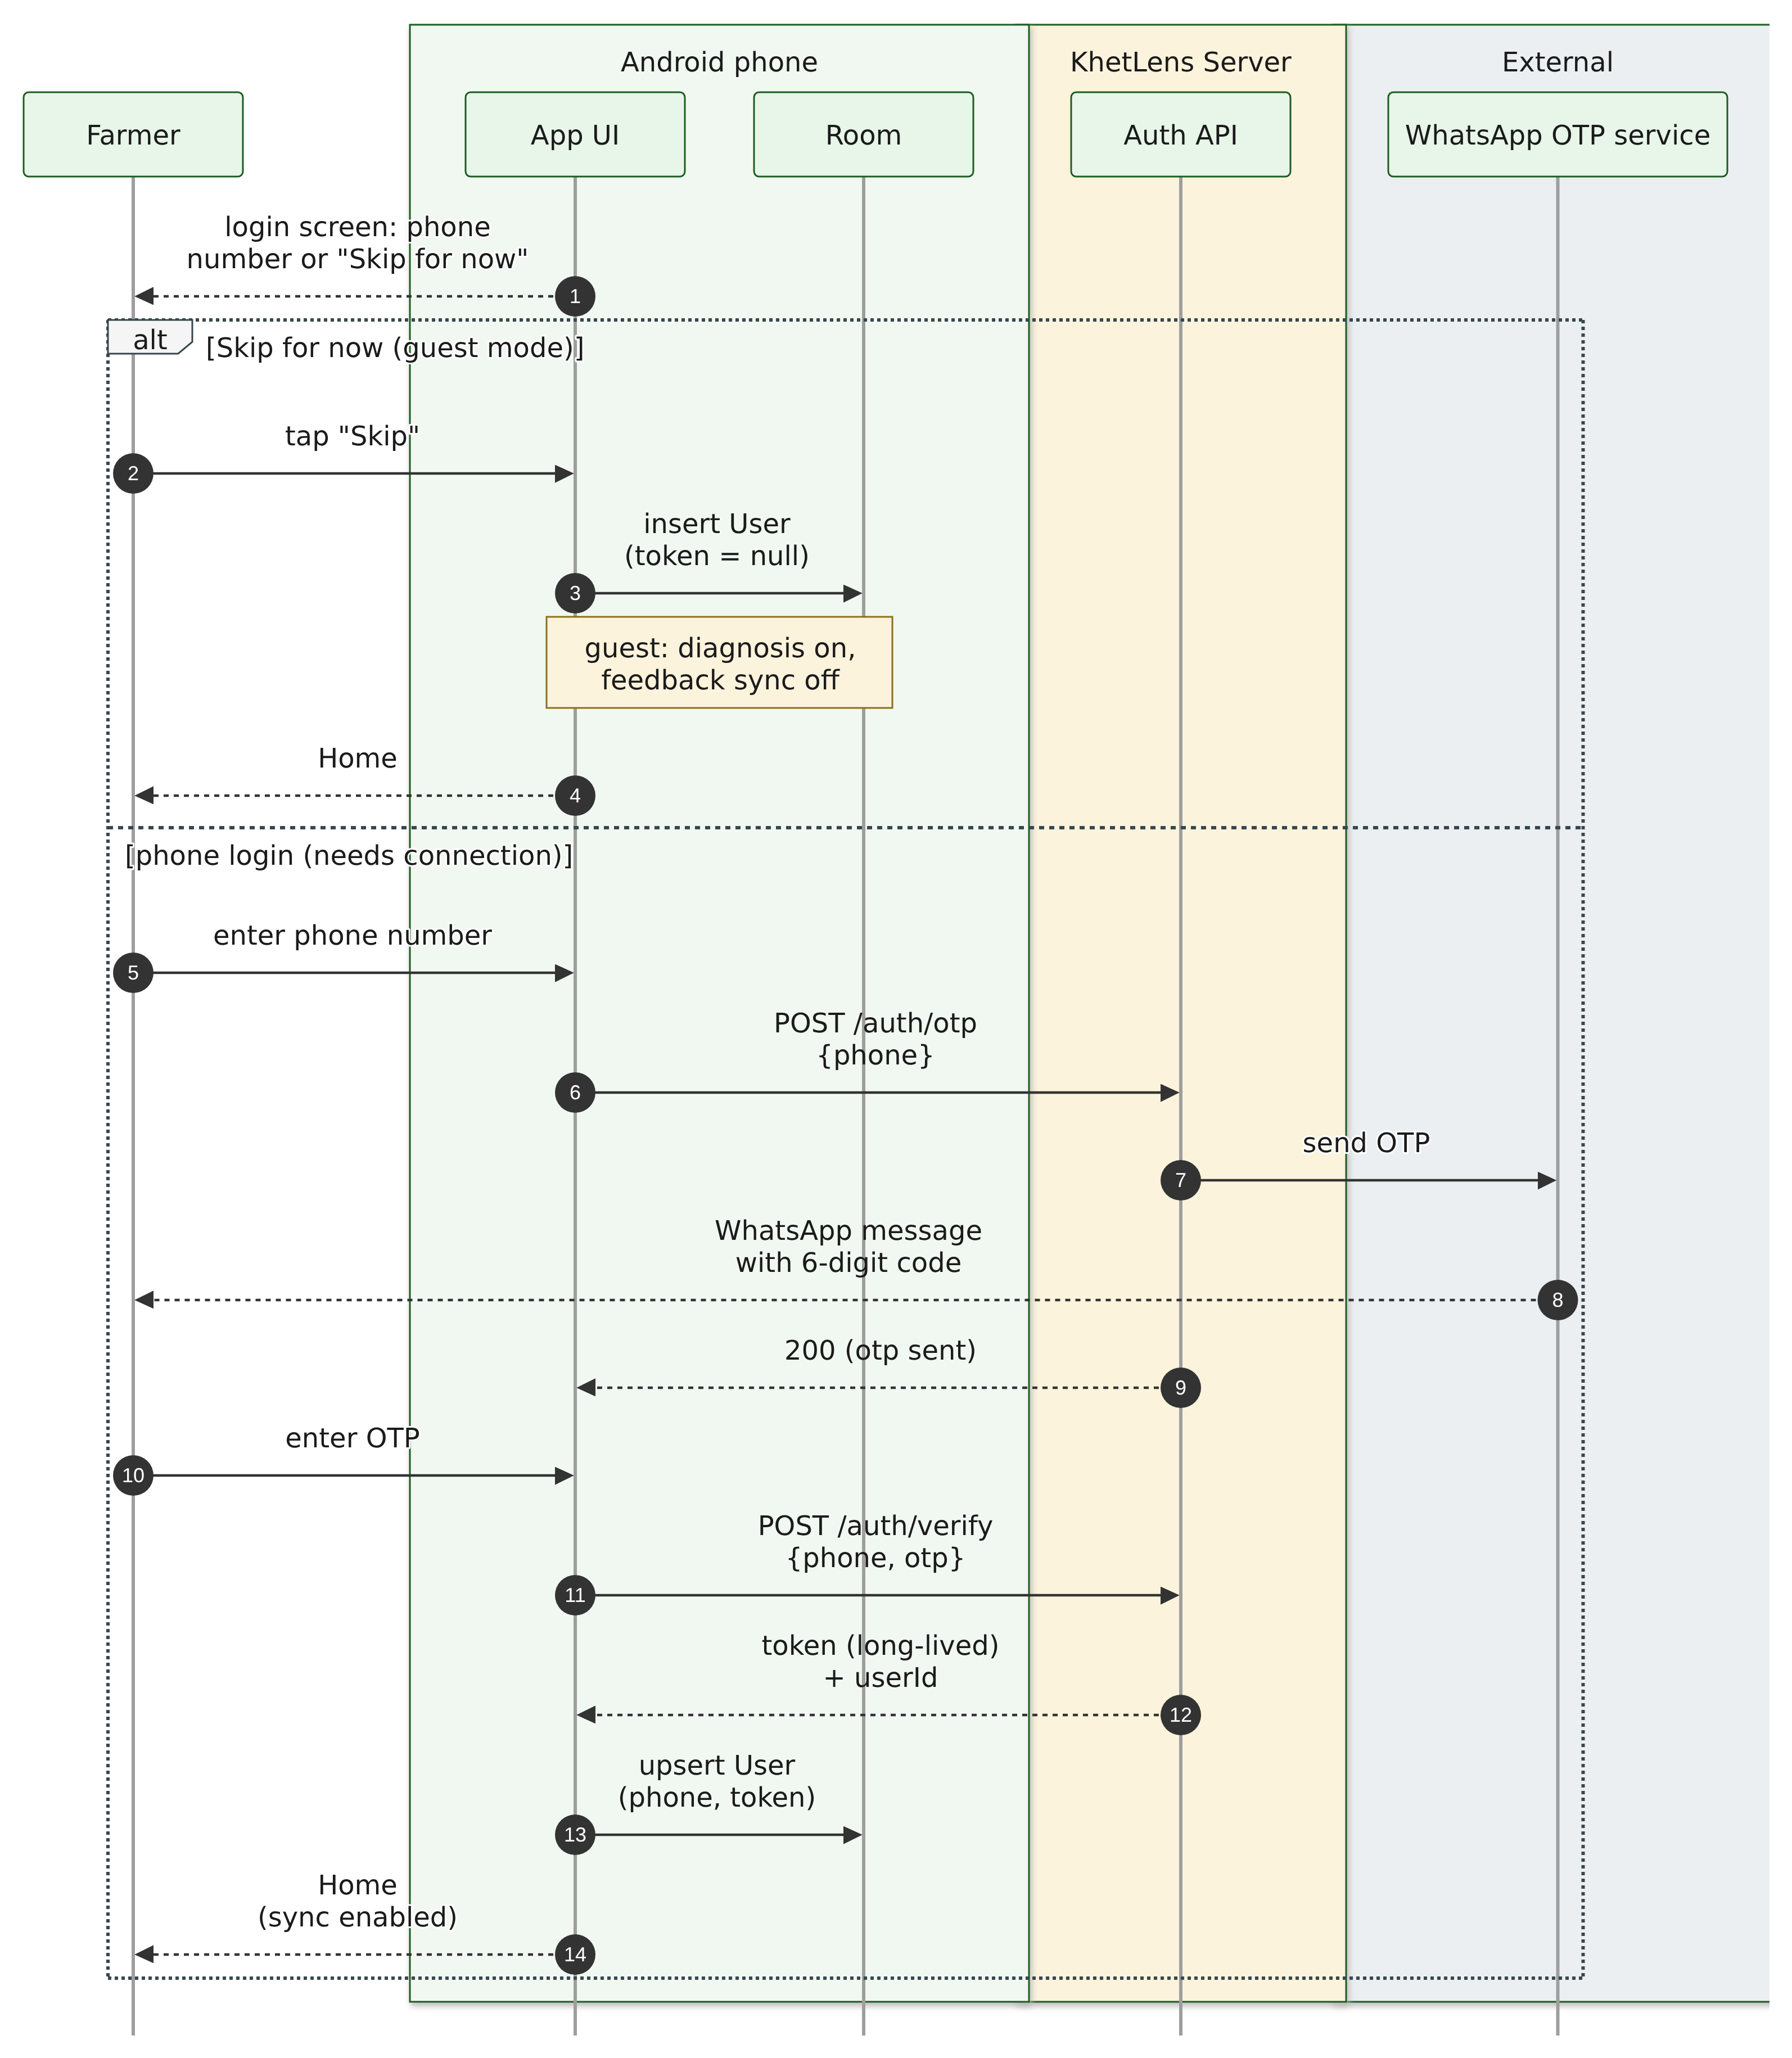
\includegraphics[width=\textwidth,height=0.88\textheight,keepaspectratio]{Figures/diagrams/seq_login.png}
  \caption{Sequence diagram for sign-in with a WhatsApp code and the guest-mode alternative.}
  \label{fig:seq-login}
\end{figure}

\textbf{Model and content update (UC-14).} Figure~\ref{fig:seq-update} shows the version check, background download, checksum verification, atomic switch and model reload, with the alternative that keeps the current version when the download fails.

\begin{figure}[H]
  \centering
  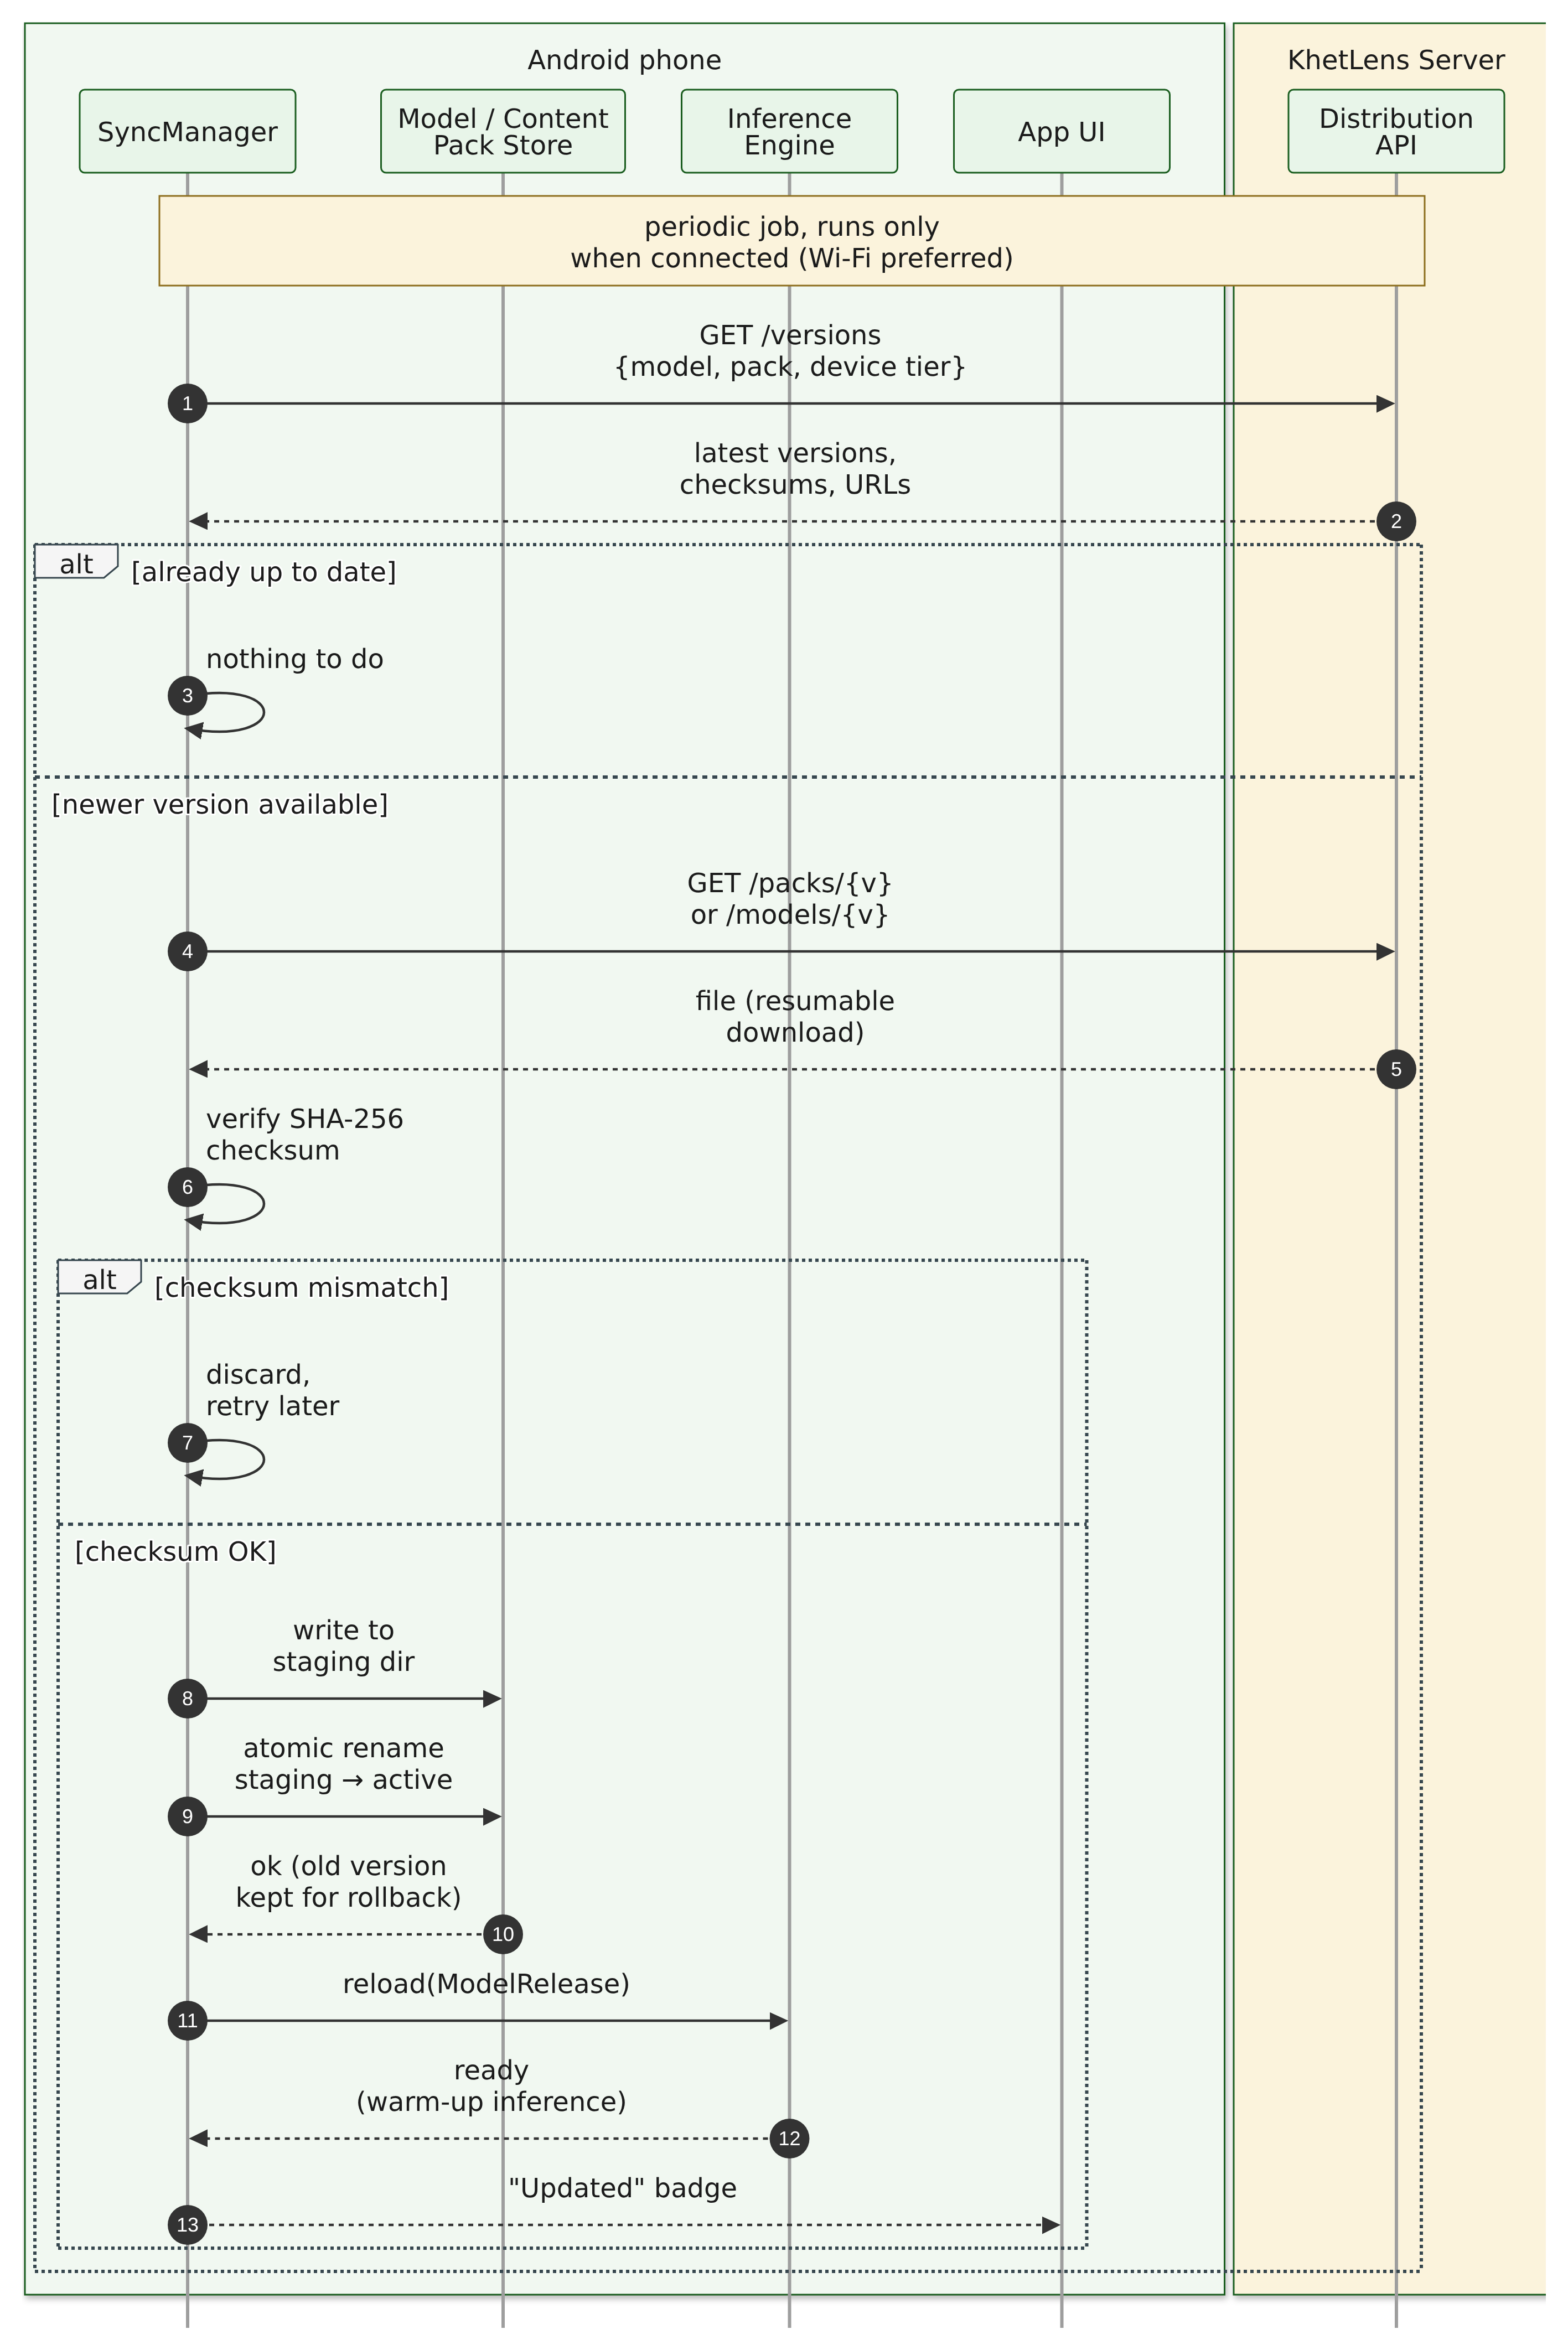
\includegraphics[width=\textwidth,height=0.88\textheight,keepaspectratio]{Figures/diagrams/seq_update.png}
  \caption{Sequence diagram for a model or content update.}
  \label{fig:seq-update}
\end{figure}

\section{Policies and Tactics}
\subsection{Conventions and coding guidelines}
Kotlin code follows the official Kotlin and Compose style guides, enforced by lint tools in the build; Python code follows PEP~8 with type hints. All user-visible strings live in resource files with Urdu and Punjabi translations. Requirement identifiers appear in test names and commit messages for traceability.

\subsection{Source layout and build}
The repository is a single project with \texttt{app/} (Android modules for presentation, domain, ML and data), \texttt{server/} (FastAPI), \texttt{training/} (data preparation, teacher, distillation, quantisation, export, calibration and the field-data study), \texttt{content/} (content sources, schema, audio) and \texttt{docs/}. A tagged release builds a signed APK and runs the test suite; model releases are produced by a single training script that runs export, calibration, contract tests and bundle creation; the publish tool uploads packs and releases to the server after validation. The APK ships with a bundled baseline model and content pack so that first launch works offline (FR-26).

\subsection{Choice of products}
TensorFlow Lite for inference (ONNX Runtime benchmarked); Room for persistence; WorkManager for background work; encrypted preferences for tokens; Noto Nastaliq Urdu and Noto Sans fonts; Opus audio; PostgreSQL; a free weather API behind a provider interface; a WhatsApp Business API provider for codes.

\subsection{Algorithms and idioms}
The diagnosis pipeline is a pure function of (image, weather, release parameters) with no hidden state, which makes it testable on the desktop with recorded inputs. Outcomes are a sealed type; repositories are interfaces; dependency injection wires the implementations.

\subsection{Requirements traceability and testing}
A traceability matrix (feature, functional requirements, use cases, design components, test cases) is kept with the documentation and will be presented in the implementation report. Unit tests cover the quality score, the thresholds, the fusion arithmetic, the question update and the repositories; contract tests load a model release and check tensor names, shapes and the manifest; instrumented tests run the farmer use cases with the network disabled; model acceptance tests compute NFR-04 and NFR-05 on the field test set for every release; farmer task tests are run with our partner's field officers.

\subsection{Maintenance and extensibility}
Adding a condition requires a new class in one disease head, a content entry and a weather-table row; adding a crop requires a new head and a new question set; changing the weather provider requires a new provider implementation. The model contract and content schema are versioned, and the app declines a release whose contract version it does not support.

\section{Conclusion}
This chapter has given the design that carries the methodology of Chapter~\ref{ch:method} to the farmer under the constraints of Chapter~\ref{ch:vision}: an offline-first native Android application with a four-layer architecture whose diagnostic core is a pure, testable function; a deliberately small backend; and an offline training pipeline whose releases are versioned artefacts consumed through a fixed contract. The architectural strategies record the alternatives we considered, the class and sequence diagrams specify the structure and behaviour at the level needed to begin implementation, and the policies define how the code will be written, tested, traced and maintained. Together with the requirements of Chapter~\ref{ch:srs}, this is the specification against which we will implement and test KhetLens.


\clearpage
\addcontentsline{toc}{chapter}{Bibliography}
{
\bibliographystyle{ieeetr}
\bibliography{fypbib}
}

\end{document}
